\documentclass[paper=a4,german,11pt,titlepage,twoside=true,headings=normal,numbers=noenddot,captions=tableabove,listof=totoc,index=totoc,bibliography=totoc]{scrreprt}
%-----------------------------------------------------------------
\usepackage{etoolbox}
\newbool{deutsch}
\booltrue{deutsch}
%-----------------------------------------------------------------
%\usepackage{amsmath} % abgesetzte Formeln zentriert in der Zeile
%\usepackage[fleqn,intlimits]{amsmath} % [fleqn] abgesetzte Formeln mit festem Abstand zum linken Rand
\usepackage{microtype}
\usepackage[reqno,intlimits]{amsmath} % [reqno] um die gleichungsnummerierung rechts zu haben
% intlimits: Grenzen für Integrale unterhalb und oberhalb des Zeichens
\usepackage{amssymb}
\usepackage{array}
\usepackage{babel}
\usepackage{varioref}
\usepackage[T1]{fontenc}
\usepackage[utf8]{inputenc}
%---------------------------
\usepackage{booktabs}
\usepackage{calc}
\usepackage{cancel}
\usepackage[labelfont={footnotesize,sf,bf},textfont={footnotesize,sf}]{caption} %Format (Textgröße, Textform) für Bildtext 
%normalsize
%scriptsize
% sc --> smallcaps
% bf --> bold face
% sf --> sans serif
\usepackage[table]{xcolor}
\usepackage[right]{eurosym}
\usepackage{ellipsis}
\usepackage{graphicx}
\usepackage{float}
%----------------------------------------
\usepackage{gensymb}
\usepackage{csquotes}
\usepackage{listings}
\usepackage{longtable}
\usepackage{lastpage}
\usepackage{lscape}
\usepackage{lmodern} %-- Silbentrennung
\usepackage{makeidx}
\usepackage{multirow}
\usepackage{multicol}
%\usepackage[intoc]{nomencl}   % zwei Spalten beim Formelzeichenverzeichnis
\usepackage[intoc]{nomentbl} %vier Spalten bei Formelzeichenverzeichnis
\usepackage{nicefrac}
\usepackage{paralist}
\usepackage{parallel}
\usepackage{pdfpages}
% Define user colors using the RGB model
%\usepackage{colortbl}
%\definecolor{dunkelgrau}{rgb}{0.8,0.8,0.8}
%\definecolor{hellgrau}{rgb}{0.95,0.95,0.95}
%\usepackage{pgfplots}
\usepackage[figuresright]{rotating} 
\usepackage{scrlayer-scrpage}
%\usepackage{sistyle}
%\usepackage[locale=DE]{siunitx} %nicht zusammen mit sistyle %---------
\usepackage[locale=DE,per-mode=symbol]{siunitx} %nicht zusammen mit sistyle %---------
% \usepackage[font={scriptsize,sl},captionskip=3pt]{subfig} % für die Unterbilder %---------
\usepackage{subcaption}
\usepackage{shortvrb}
\usepackage{tablefootnote}
\usepackage{tabularx}
\usepackage{tabulary}
\usepackage{textcomp}
\usepackage{tocbasic}
\usepackage{tikz}
\usepackage{times} 
\usepackage{units} %----------
\usepackage{xurl}
\usepackage{wrapfig} %----------
\usepackage{xr-hyper}
\usepackage{arydshln} %für \hdashline[5pt/2pt] % muss am Ende stehen, sonst gibt es Probleme mit xcolor
\usepackage{hyperref} % muss am Schluss stehen
\hypersetup{
    colorlinks=true, % Color links instead of disgusting boxes :barfing_emoji:
    linkcolor={black}, % Color of internal links
    citecolor={black}, % Color of citations
    urlcolor={blue} % Color of external hyperlinks
}
%\usepackage{unicode-math}
%\usepackage[toc,symbols]{glossaries} %---------- muss nach hyperref stehen
\usepackage[nonumberlist, acronym, toc, section]{glossaries} % muss nach hypersetup stehen
%----------------
%\usepackage{romannum} % Seitenzahlen in römischen Ziffern
%\usepackage{adjustbox}
\usepackage{scrhack}
\usepackage[style=numeric, citestyle=numeric, backend=biber]{biblatex}
\usepackage[useregional]{datetime2}
\usepackage{cleveref} % löscht labels!!!!!!!!!! <--- warum? habs trotzdem eingefügt weil es die referencen nice macht ohne newcommands dafür zu brauchen. außerdem steht intellisense drauf ;)
% \usepackage{isotope} % um chemische gleichungen hübscher darstellen zu können
\usepackage{framed} % rahmen um dinge malen können
\usepackage{svg} % um auch vektorgrafiken als bild einfügen zu können
\usepackage{adjustbox} % skaliert floats dynamischer (anti-over/underfull)
\usepackage[numbered]{bookmark} % platziert im pdf reader bei der kapitelübersicht die jeweiligen kapitelnummer vor die kapitelüberschriften
% ---------- Make floats stay within the chapter/section/subsection they got placed ------------------
\usepackage{placeins}
\let\Oldsection\section
\renewcommand{\section}[1]{\FloatBarrier\Oldsection{#1}}
\let\Oldsubsection\subsection
\renewcommand{\subsection}[1]{\FloatBarrier\Oldsubsection{#1}}
\let\Oldsubsubsection\subsubsection
\renewcommand{\subsubsection}[1]{\FloatBarrier\Oldsubsubsection{#1}}
%===================== define VARIABLES ==========================
% --------------------- Names ------------------------------------
\newcommand{\thefirstnameA}{Dennis}
\newcommand{\thelastnameA}{Hunter}
\newcommand{\thefirstnameB}{David}
\newcommand{\thelastnameB}{Ickstadt}
\newcommand{\thefirstnameC}{Cihan}
\newcommand{\thelastnameC}{Ünlü}
% --------------------- Titel Course -----------------------------
\newcommand{\titleLV}{Gerätekonstruktion B}
%---------------------- Document Titel ---------------------------
\newcommand{\subtitleA}{SnookerBot\par\vspace{0.4cm}a.k.a.}
\newcommand{\subtitleB}{"Yet Another Bot"}
%---------------------- Dates ------------------------------------
% \newcommand{\versuch}{2} % Versuchsnummer einfügen
\newcommand{\dateLV}{17.11.2020} % Datum einfügen
\newcommand{\deadline}{28.02.2022} % Abgabedatum ist der 1.12.2020
% \newcommand{\dateLVa}{December 1st, 2020}
% \newcommand{\dateLVb}{December 8th, 2020}
%:::::::::::::::::::::::::::::::::::::::::::::::::::::::::::::::::
%-------------------------
 %\renewcommand{\captionlabelfont}{\sffamily} %für "Abbildung" und "Tabelle"
 %\renewcommand{\captionfont}{\sffamily\small} %für den Text der Bildunterschriften
%  \renewcommand{\captionlabelfont}{\sffamily} 
%  \renewcommand{\captionfont}{\sffamily} %\renewcommand{\normalfont}{\sffamily} %für die Überschriften
% Fettdruck der Bezeichnung Abbildung, Tabelle
%\renewcommand{\captionlabelfont}{\bfseries}
%---------------------------------------------
%------------------ Schrifttyp in der Kopf- und Fusszeilen
\setkomafont{pageheadfoot}{\footnotesize\sffamily}
%---------------------------------------------------
%Ändern der Abbildung- und Tabellenbezeichnung (Niedermair S.157)
%_____________________________________________
\ifbool{deutsch}{%
\addto\captionsngerman{\renewcommand\figurename{Abb.}}
\addto\captionsngerman{\renewcommand\tablename{Tab.}}
\renewcommand\listfigurename{Abbildungen}
}{}
%_______________________________
%Betrag eines Wertes
% \newcommand{\abs}[1]{\lvert #1 \rvert}
%---------------------------------------------
% \newcommand{\absatz}[1]{\textbf{\textsc{#1}}} %siehe Mittelbach S. 876ff
%----------------------------
%\newcommand{\absatz}{\par \medskip}
%______________________________
%\newcommand{\anhang}[1]{Anhang \ref{#1}, Seite \pageref{#1}}
% \newcommand{\anhang}[1]{Anhang \vref{#1}}
% %________________________________
% \newcommand{\aufgabe}{\stepcounter{plus} Aufgabe \arabic{plus}}
%______________________________________
%compactitem
% \newcommand{\bci}{\begin{compactitem}}
% \newcommand{\eci}{\end{compactitem}}
% %______________________________________
% %
% \newcommand{\bi}{\begin{itemize}}
% \newcommand{\ei}{\end{itemize}}
% %______________________________________
% %compactenumerate
% \newcommand{\bce}{\begin{compactenum}}
% \newcommand{\ece}{\end{compactenum}}
% %_____________________________________
% %begin equation
% \newcommand{\be}{\begin{equation}}
% \newcommand{\ee}{\end{equation}}
% %_____________________________________
% %begin equation ohne Formelnummer
% \newcommand{\ben}{\begin{equation*}}
% \newcommand{\een}{\end{equation*}}
% %_____________________________________
% %begin align ohne Formelnummer
% \newcommand{\ban}{\begin{align*}}
% \newcommand{\ean}{\end{align*}}
%_____________________________________
%begin align
% \newcommand{\ba}{\begin{align}}
% \newcommand{\ea}{\end{align}}
%_____________________________________
%minpage
% \newcommand{\bmp}{\begin{minipage}[t]{.47\linewidth}}
% \newcommand{\emp}{\end{minipage}}
%_____________________________
%  dB
% \newcommand{\db}{dB}
% %  dB(A)
% \newcommand{\dba}{ dB(A) }
% %  dB(A) für Satzende
% \newcommand{\dbap}{ dB(A)}
% %_________________________________
% \newcommand{\bzw}{bzw.\,}
% %_______________________________
% \newcommand{\dif}{\mathrm{d}}
%________________________________
% neuer Zähler
\newcounter{plus}
\setcounter{plus}{0}
%______________________________
%Für das Formelverzeichnis _____________________ Formelverzeichis ____
% Befehl umbenennen in fz
% \let\fz\nomenclature
% Deutsche Überschrift
\ifbool{deutsch}{%
\renewcommand{\nomname}{Formelzeichen}
}{}
% Punkte zw. Abkürzung und Erklärung
\setlength{\nomlabelwidth}{.20\hsize}
\renewcommand{\nomlabel}[1]{#1 \dotfill}
% Zeilenabstände verkleinern
\setlength{\nomitemsep}{-\parsep}
%_____________________________
% \newcommand{\bild}[1]{Abb. \vref{#1}}
% \newcommand{\sbild}[1]{siehe Abb. \vref{#1}}
% \newcommand{\bilder}[2]{Abb. \vrefrange{#1}{#2}}
% \newcommand{\bildseite}[1]{Abb. \vref{#1}} % erzeugt "`Abb. nn auf Seite nn
% \newcommand{\tabelle}[1]{Tab. \vref{#1}}
% \newcommand{\tabellenseite}[1]{Tab. \vref{#1}} % erzeugt "`Tab. nn auf Seite nn
% für \vref ist usepackage[german]{varioref} einzufügen
%_-------------------------------- Freiraum
% \newcommand{\freiraum}[1]{\begin{figure}[H]\vspace{#1\textheight}\end{figure}}
%_____________________________
% Gleichung
% \newcommand{\gl}[1]{Gl.\,(\ref{#1})}
% \newcommand{\sgl}[1]{siehe Gl.\,(\ref{#1})}
% \newcommand{\glbereich}[2]{Gl. \vrefrange[]{#1}{#2}}
%_____________________________
% Grad Celsius
% \newcommand{\grad}{\,\degC}
% \newcommand{\gradC}{\,\degree}
%______________________________________
% Großbuchstaben als Indizes kleiner schreiben; spezielle im Mathemodus
% \newcommand{\klein}[1]{\scriptscriptstyle{#1}}% Fettdruck der Bezeichnung 
%______________________________
%% Kasten
% \newcommand{\kasten}{\fbox{\rule{0.0pt}{10pt}{{ } } }}
%______________________________
%\newcommand{\kapitel}[1]{Kapitel \ref{#1}, Seite \pageref{#1}}
% \newcommand{\kapitel}[1]{Kapitel \vref{#1}}
%_____________________________
%  LAeq für den äquivalenten Dauerschallpegel
% \newcommand{\laeq}{ $L_{Aeq}$ }
%  LAeq für den äquivalenten Dauerschallpegel am Satzende
% \newcommand{\laeqp}{ $L_{Aeq}$}
%_________________________________
%   Linie zeichnen
\newcommand{\linie}{\rule{0.5\textwidth}{0.1pt}}
%---------------------- LaTeX
% \newcommand{\lt}{\LaTeX\,\,}
%----------------------------
% \newcommand{\nl}{\newline}
%__________________________________
%  multicolumn für Tabellen
% \newcommand{\mc}{\multicolumn}
%% \mc{1}{c}{Text}
%_________________________________
%    Parallel
% \newcommand{\pl}[1]{\ParallelLText{#1}}
% \newcommand{\pr}[1]{\ParallelRText{#1}}
% \newcommand{\pp}{\ParallelPar}
%------------ rot unterstrichen
% \newcommand{\rotunterstrichen}[1]{\textcolor{red}{\underline{\textcolor{black}{#1}}}}
%________________ Realteil
% \newcommand{\real}[1]{\text{Re}\left\{#1\right\}}
%________________________________--
% \newcommand{\seite}[1]{Seite \pageref{#1}}
% \newcommand{\seiten}[2]{\vpagerefrange{#1}{#2}}
%----------------------------
%        TEXT Rot
\newcommand{\textrot}[1]{\textcolor{red}{#1}}
%______________________________
%Abkürzung für \multicolumn
% \newcommand{\tab}[2]{\multicolumn{1}{#1}{#2}}
%_____________________________________
% doppelt unterstreichen
% \newcommand{\unterstreichen}[1]{\underline{\underline{#1}}}
% einfach unterstreichen
% \newcommand{\ul}[1]{\underline{#1}}
%______________________________
%kurze Verbatimausgabe
%\MakeShortVerb{\|} %mittelbach S.160 mit \usepackage{shortvrb}
%_______________________________________
% vspace
% \newcommand{\vsf}{\vspace{5pt}}
%_________________________________
% \newcommand{\zb}{z.B.\,}
% \newcommand{\idr}{i.d.R.\,}
%_______________________________
% Zähler-einfach
\newcounter{req}
% \newcommand{\zaehler}[1]{\refstepcounter{req}{#1} \thereq}
%% Beispielaufzählung \zaehler{Beispiel}\\
%_____________________________________
%A4: 210x297 (BxH)
% \setlength{\voffset}{-2.532 cm}
% \setlength{\hoffset}{-1.57 cm}
\setlength{\voffset}{-2.5 cm}
\setlength{\hoffset}{-2 cm}
% \setlength{\topmargin}{2.0 cm} \setlength{\topskip}{0.1 cm}
\setlength{\topmargin}{1.5 cm}
\setlength{\topskip}{0.1 cm}
\setlength{\evensidemargin}{1.5 cm}
\setlength{\oddsidemargin}{1.5 cm}
%  \setlength{\textwidth}{16.5 cm}
\setlength{\textwidth}{16.0 cm}
\setlength{\footskip}{40pt}
\setlength{\textheight}{24.7cm}
% \setlength{\textheight}{23.5 cm}
\setcounter{page}{1}
\setlength{\parindent}{0cm}
\setlength{\headsep}{20pt}
%----------------------------------------------------------------------
% Linien in der Kopf- und Fußzeile
%\renewcommand{\headrulewidth}{0.0pt}   %Linie in der Kopfzeile mit 0.0pt keine Linie
%%\renewcommand{\footrulewidth}{0.0pt}   %Linie in der Fußzeile mit 0.0 pt keine Linie
%\renewcommand{\headrulewidth}{0.2pt}   %Linie in der Kopfzeile mit 0.0pt keine Linie
%\renewcommand{\footrulewidth}{0.2pt}   %Linie in der Fußzeile mit 0.0 pt keine Linie
%------------------------------------------------------------------------
%\renewcommand{\normalfont}{\sffamily} %für die Überschriften
%\renewcommand{\chaptermark}[1]{\markboth{\chaptername\ \thechapter #1}{}}
%\renewcommand{\sectionmark}[1]{\markright{\thesection\ #1}}
% \rfoot{\leftmark\\\rightmark}

%Definitionen für Kopfzeile
% bei documentclass {report} hat der Eintrag für die [gerade Seite] keine Wirkung
%-------------------------------------------------------------
%%
%Einstellungen für Kopf- und Fusszeilen mit dem KOMA-Skript und \usepackage{scrpage2}
\pagestyle{scrheadings}
%\pagestyle{scrplain}
% le --> links, gerade Seite
% ce --> mittig, gerade Seite
% re --> rechts, gerade Seite
% lo --> links, ungerade Seite
% co --> mittig, ungerade Seite
% ro --> rechts, ungerade Seite
%---------------------------------------------
% Löschen aller Einträge
%\clearscrheadings
% \automark[section]{subsection}
% \pagemark --> Seitenzahl
% \automark --> Kapitelüberschriften
% \leftmark --> ??
% \rightmark --> ??
%::::::::::::::::::::::::::::::::::: Kopfzeile
% Kopfzeile gerade Seite
\automark[chapter]{chapter}
\lehead[]{\titelkopfzeilelinkseven}
\cehead[]{\titelkopfzeilemitteeven}
\rehead[]{\titelkopfzeilerechtseven}
% Kopfzeile ungerade Seite
\lohead[]{\titelkopfzeilelinksodd}
\cohead[]{\titelkopfzeilemitteodd}
\rohead[]{\titelkopfzeilerechtsodd}
% Linie in der Kopfzeile
%\setheadtopline{0.2pt} % obere Linie in der Kopfzeile; nur bei scrartcl
%\setheadsepline{0.4pt} % untere Linie in der Kopfzeile; nur bei scrartcl
\KOMAoptions{headsepline=0.4pt}
% Linie in der Fusszeile
%::::::::::::::::::::::::::::::::::: Fußzeile
% Fusszeile gerade Seite[plain-style]{scrheadings-style}
\lefoot[]{\titelfusszeilelinkseven} 
\cefoot[]{\titelfusszeilemitteeven}
\refoot[]{\titelfusszeilerechtseven}
% Fusszeile ungerade Seite
\lofoot[]{\titelfusszeilelinksodd}
\cofoot[]{\titelfusszeilemitteodd}
\rofoot[]{\titelfusszeilerechtsodd}
%\rofoot[\thepage ]{\thepage}
%\setfoottopline{0.2pt} % obere Linie in der Kopfzeile; nur bei scrartcl
%\setfootsepline{0.4pt} % untere Linie in der Kopfzeile; nur bei scrartcl
\KOMAoptions{footsepline=0.4pt}

% le --> links, gerade Seite
% ce --> mittig, gerade Seite
% re --> rechts, gerade Seite
% lo --> links, ungerade Seite
% co --> mittig, ungerade Seite
% ro --> rechts, ungerade Seite
% even --> gerade Seite
% odd --> ungerade Seite
%----------------------------------------- Kopfzeilentext
 \newcommand{\titelkopfzeilemitteeven}{}
 \newcommand{\titelkopfzeilemitteodd}{}
 \newcommand{\titelkopfzeilelinkseven}{Hochschule RheinMain}
 \newcommand{\titelkopfzeilelinksodd}{}
 \newcommand{\titelkopfzeilerechtseven}{}
 \newcommand{\titelkopfzeilerechtsodd}{Hochschule RheinMain}
 %----------------------------------------- Fußzeilentext
 \newcommand{\titelfusszeilemitteeven}{}
 \newcommand{\titelfusszeilemitteodd}{}
 \newcommand{\titelfusszeilerechtseven}{Studienbereich Angewandte Physik \& Medizintechnik}
 \newcommand{\titelfusszeilerechtsodd}{\thepage \hspace{0.5mm} von \pageref{LastPage}}
 \newcommand{\titelfusszeilelinkseven}{\thepage \hspace{0.5mm} von \pageref{LastPage}}
 \newcommand{\titelfusszeilelinksodd}{Studienbereich Angewandte Physik \& Medizintechnik}
%
%=====================Code Listing Layout Matlab=============================
\definecolor{codegreen}{RGB}{28,172,0} % color values Red, Green, Blue
\definecolor{codelilas}{RGB}{170,55,241}
\lstdefinestyle{matlab}{language=Matlab,%
    basicstyle=\footnotesize,%
    inputencoding=latin1,%
    breaklines=true,%
    stepnumber=2,% line numbering steps
    morekeywords={ones,height,width,datetime},% additional keywords to highlight
    keywordstyle=\color{blue},%
    frame=none,%
    identifierstyle=\color{black},%
    stringstyle=\color{codelilas},%
    commentstyle=\color{codegreen},%
    showstringspaces=false,%without this there will be a symbol in the places where there is a space
    numbers=left,%
    numberstyle={\tiny \color{black}},% size of the numbers
    numbersep=9pt,% this defines how far the numbers are from the text
}
\lstdefinestyle{python}{language=Python,%
    basicstyle=\footnotesize,%
    inputencoding=latin1,%
    breaklines=true,%
    stepnumber=2,% line numbering steps
    morekeywords={ones,height,width,datetime},% additional keywords to highlight
    keywordstyle=\color{blue},%
    frame=none,%
    identifierstyle=\color{black},%
    stringstyle=\color{codelilas},%
    commentstyle=\color{codegreen},%
    showstringspaces=false,%without this there will be a symbol in the places where there is a space
    numbers=left,%
    numberstyle={\tiny \color{black}},% size of the numbers
    numbersep=9pt,% this defines how far the numbers are from the text
}
%==============================================================================
\DeclareNameAlias{author}{family-given}
\DeclareNameAlias{editor}{family-given}
\DeclareNameAlias{translator}{family-given}
\addbibresource{quellen.bib}
%------DEBUGGING--------------------------------------------------
% \usepackage[showframe]{geometry} % comment for live version
% \usepackage{layout}
% \usepackage{showframe}
%-----------------------------------------------------------------
\begin{document}
%-----------------------------------------------------------------
\begin{titlepage}
	% -------- Naming ------------------------------
	\ifbool{deutsch}{%
		\newcommand{\nameA}{\thefirstnameA\space\thelastnameA}
		\newcommand{\nameB}{\thefirstnameB\space\thelastnameB}
		\newcommand{\nameC}{\thefirstnameC\space\thelastnameC}
	}{%
		\newcommand{\nameA}{\thelastnameA\,\space\thefirstnameA}
		\newcommand{\nameB}{\thelastnameB\,\space\thefirstnameB}
		\newcommand{\nameC}{\thelastnameC\,\space\thefirstnameC}
	}
	% ----------------------------------------------
	\newcommand{\HRule}{\rule{\linewidth}{0.5mm}}
	\centering
	\textsc{\Large Hochschule RheinMain} \par
	\begin{center}
		
\includegraphics[width=0.15\textwidth]{logo-hsrm.jpg}
	\end{center}
	\textsc{\LARGE \titleLV}\vspace{0.5cm}
		\HRule\vspace{0.4cm}
	{\huge\bfseries \subtitleA}\par\vspace{0.4cm} % Title of Document
	{\huge\bfseries \subtitleB}\par\vspace{0.4cm} % Titel des Dokuments
		\HRule\vspace{1.5cm}
%-------------------
\begin{minipage}{0.4\textwidth}
	\large
	\ifbool{deutsch}{%
		\textit{\underline{Autoren}}\par\vspace{0.5cm}
	}{%
		\textit{\underline{Author}}\par\vspace{0.5cm}
	}
	\textsc{\nameA}\par\vspace{0.5cm}
	\textsc{\nameB}\par\vspace{0.5cm}
	\textsc{\nameC}\par\vspace{0.5cm}
\end{minipage}
%------------------------------------
\vfill\vfill\vfill
\ifbool{deutsch}{%
	\textsc{\Large Fachbereich Ingenieurwissenschaften}\vspace{0.5cm}\par
	\textsc{\large Studienbereich Angewandte Physik \& Medizintechnik}\vspace{0.5cm}
	\vfill
	\begin{flushleft}
		Abgabedatum:\hspace{0.4cm} {\large\today}
	\end{flushleft}
}{%
	\textsc{\Large Department of Engineering}\par\vspace{0.5cm}\par
	\textsc{\large Applied Physics \& Medical Technology}\par\vspace{0.5cm}
	\vfill
	\begin{flushleft}
		Date:\hspace{0.4cm} {\large\today}
	\end{flushleft}
}
\end{titlepage}
\pagenumbering{Roman}
\tableofcontents
\newpage
\addchap{Kurzzeichenverzeichnis}
    \begin{table}[h]
        \begin{tabular}{@{}ll@{}}%
            \(a_T\) & Tangentialbeschleunigung\\
            \(b\) & Strecke Drehachse - Angriffspunkt PAM\\
            \(l_{eff}\) & Strecke zwischen Drehachse Schulter und Aufhängung Queue\\
            \(l_o\) & Länge des Oberarms\\
            \(l_u\) & Länge des Unterarms\\
            \(m\) & bewegte Masse des Arms\\
            \(m_{Kugel}\) & Masse der Billardkugel\\
            \(m_o\) & Masse des Oberarms\\
            \(m_u\) & Masse des Unterarms\\
            \(s_m\) & Massenschwerpunkt entlang des Unterarms\\
            \(v\) & Stoßgeschwindigkeit des Arms\\
            \(v_{Kugel}\) & Geschwindigkeit der Kugel\\
            \(v_{Stoss}\) & Geschwindigkeit des Stoßes\\
            \(x_s\) & Massenschwerpunkt des Oberarms, Unterarms und Queues\\
            \(x_o\) & Massenschwerpunkt des Oberarms\\
            \(x_u\) & Massenschwerpunkt des Unterarms\\
            & \\
            \(B\) & Strecke Drehachse - Ende des Unterarms\\
            \(F\) & erforderliche Kraft des PAMs\\
            \(F_x\) & Kraft am Unterarm in X-Richtung\\
            \(F_{Stoss}\) & Stärke des Stoßes\\
            \(I\) & Trägheitsmoment des Arms\\
            \(M\) & Drehmoment Arm\\
            \(M_m\) & Verursachtes Drehmoment Schulter\\
            \(N\) & Untersetzung\\
            \(Z_1\) & Anzahl Zähne der inneren Scheibe\\
            \(Z_2\) & Anzahl Zähne der äußeren Scheibe\\
            & \\
            \(\alpha\) & Winkelbeschleunigung\\
            \(\alpha_T\) & Tangentialbeschleunigung\\
            \(\beta\) & Winkel PAM Oberarm\\
            \(\Delta s_{arc}\) & Verfahrbare Mindestbahnlänge\\
            \(\Delta x\) & Ausholstrecke beim Stoß
    \end{tabular}\label{tab:glossar}
    \end{table}
%-----------------------------------------------------------------
% \newcommand{\chaptercount}{5} % put number of chapters here
% \foreach \c in {1,...,\chaptercount}{\input{chapters/\c_chap}}
\clearpage\pagenumbering{arabic}
% Die Einleitung umfasst eine Hinführung zum Thema und sollte die Relevanz der Aufgabenstellung in ihrem wissenschaftlichen Kontext herausstellen. Darüber hinaus sollte an dieser Stelle Bezug auf die Problemstellung genommen und dem Leser ein kurzer Ausblick auf die Arbeit vermittelt werden (in der Form: „Was erwartet den Leser?“). Der Umfang soll 3 Seiten nicht übersteigen.
\chapter{Einleitung}
	
	Billard ist ein Spiel, in dem Kugeln durch Stoßen einer anderen, weißen Kugel in die Taschen an den Ecken und den langen Seiten des Billardtischs versenkt werden. Dabei führt der Spieler mit einem Arm durch Führen des sogenannten Queues einen Stoß durch, während es von der Hand des anderen Arms gestützt wird.\\
	Profispieler wollen durch Erfahrung und Expertise nach einer perfekten Haltung streben. Dabei spielt der Arm eine ganz wichtige Rolle, da er fast für den ganzen Erfolg des Stoßes verantwortlich ist. Genau deshalb ist es für einen Spieler auch wichtig seine Haltung analysieren zu können und Verbesserungsmöglichkeiten aufgezeigt zu bekommen.\\
	Dies soll durch einen den Spieler unterstützenden Mechanismus geschehen. Es ist ein System gegeben, welches den Stoß eines Spielers aufzeichnen und zur Nachahmung weitervermittelt werden kann. Durch die Aufzeichnung des Verhaltens ist der Spieler in der Lage, sinnvolle Rückmeldung zu seiner Haltung, Durchführung und Sonstiges zu erhalten und diese zu verbessern. Um dies zu erreichen, muss eine dem Menschen ähnliche Struktur des Arms realisiert und zur Anwendung bereitgestellt werden.\\
	Um diesen Anforderungen gerecht zu werden, wird in diesem Bericht eine Lösungsmethode für die aufkommende Problemstellung ausgearbeitet. Dabei wird darauf geachtet, dass die Anatomie und Ergonomie eines echten Menschen beim Stoß einer Billardkugel mit einem Queue berücksichtigt wird.\\
	Idealerweise wird eine Konstruktion erhalten, welche alle Fähigkeiten und Eigenschaften eines Menschen beinhaltet und diese je nach Bedarf angepasst werden können.

% Im Theorieteil ist der aktuelle Stand der Technik/Forschung wertungsfrei darzustellen. Er dient dazu, den wissenschaftlichen Kontext für die Aufgabenstellung herauszuarbeiten. Dementsprechend sollte die Darstellungsweise nicht zu allgemein gewählt werden, sondern nur die für die Aufgabenstellung relevanten Theorien und notwendigen Definitionen dargelegt werden. Stehen mehrere Theorien zur Verfügung, ist ein Überblick zu geben. Definitionen sind nur dann notwendig, wenn sie nicht ohnehin als allgemein, d.h. von Vertreter des Fachbereichs, bekannt vorausgesetzt werden können und für den weiteren Verlauf der Arbeit relevant sind. Die Theorie hat einen entscheidenden Einfluss auf die Methodenwahl und die Interpretation der Ergebnisse. Der Stand der Technik ist u.a. dokumentiert in Monografien, Vortragsmanuskripten, Patenten und in besonderer Weise in Artikeln wissenschaftlicher Zeitschriften. Diese Quellen Seite 5 sind zu nutzen. Es wird eine Analyse von mindestens vier Zeitschriftenartikeln erwartet, von denen mindestens einer in englischer Sprache verfasst ist. Bei der Auswahl der Literatur ist auf Aktualität der Arbeiten zu achten.
\chapter{Theorie}
	\section{Theorie zur Auslegung der künstlichen Muskeln}
		Um die Baugruppe an die Bewegungen eines Billiardspielers anzupassen, müssen die Bauteile entsprechend ausgelegt werden. 
		Dazu zählt unter anderem die Auslegung der Kraft der künstlichen Muskeln. 
		Um dies richtig erfassen zu können wurde ein schematischer Aufbau des Arms angenommen und daran die Berechnungen ausgeführt. 
		Zunächst allerdings wird der Impuls, den der Billiardqueue auf die Spielkugel überträgt betrachtet. 
		Dabei gilt, dass die beiden Impulse bei unterschiedlicher Masse und Geschwindigkeiten identisch sind. 
		\begin{equation}
			m_{Arm} \cdot v_{Arm} = m_{Kugel} \cdot v_{Kugel}%
			\label{eq:ImpulsKugel}
		\end{equation}
		Dabei ist die Masse des Arms \(m_{Arm}\), die Bewegungsgeschwindigkeit des Arms \(v_{Arm}\), die Masse der Kugel \(m_{Kugel}\) und die Bewegungsgeschwindigkeit der Kugel \(v_{Kugel}\).
		Damit kann die benötigte Bewegungsgeschwindigkeit an der Hand des Armes berechnet werden.
		\begin{equation}
			v_{Arm} = \frac{m_{Kugel} \cdot v_{Kugel}}{m_{Arm}}%
			\label{eq:SollgeschwindikeitArm}
		\end{equation}

		Die kann dann dazu genutzt werden die erforderliche Kraft der pneumatischen Muskeln zu berechnen.
		Sie ist im folgenden mit \(v\) für die Sollgeschwindigkeit bezeichnet. \par
		Nun wird über das Drehmoment die benötigte Kraft der künstlichen Muskeln oder auch PAMs berechnet. 



		\begin{equation}
			M = b \cdot F = I \cdot \alpha%
			\label{eq:DrehmomentArm}
		\end{equation}

		mit dem Trägheitsmoment \( I = m \cdot s_m^2 \), der Tangentialbeschleunigung \( a_T = \frac{v^2}{\Delta x} \) und der
		Winkelbeschleunigung \( \alpha = \frac{a_T}{B} \) \par\medskip

		\begin{align}
			I \cdot \frac{a_T}{B} &= m \cdot s_m^2 \cdot \frac{a_T}{B} \nonumber\\
			b \cdot F &= m \cdot s_m^2 \cdot \frac{a_T}{B} \nonumber\\
			F &=\frac{m \cdot {s_m}^2 \cdot a_T}{B \cdot b \cdot cos(\beta)}%
			\label{eq:Kraft-PAM}
		\end{align}

		Eine Skizze zur Veranschaulichung, sowie die Beschreibungen der Variablen befinden sich auf der nächsten Seite. 

		\newpage
		\begin{figure}[h]
			\centering
			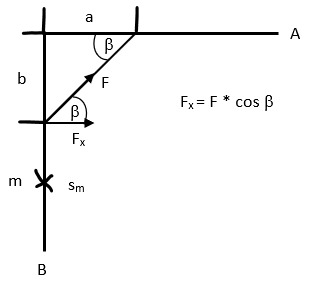
\includegraphics[width=.5\textwidth]{Abb/SkizzeBerechnungen.jpeg}
			\caption{Skizze Berechnungen.}%
			\label{fig:SkizzeBerechnungen}
		\end{figure}

		Hier sind

		\( m := \) Masse Unterarm \\
		\( s_m := \) Massenschwerpunkt entlang $ B $ \\
		\( v := \) Soll-Endgeschwindigkeit \\
		\( \Delta x := \) Ausholstrecke vor dem Stoß \\
		\( B := \) Strecke Drehachse - Ende des Unterarms \\
		\( b:= \) Strecke Drehachse - Angriffspunkt PAM \\
		\( \beta := \) Winkel PAM  Oberarm \\
		\( F:= \) Erforderliche Kraft des PAM

	\section{Theorie zur Auslegung des Schultergetriebes}
		Um den Queue korrekt anlegen zu können ist es erforderlich, dass sämtliche Unterbaugruppen vor, während und nach eines Stoßes in der eingestellten Ausrichtung verharren.
		Weiter muss die angestrebte Position an der Kugel, sowie der Stoßwinkel in ausreichender Präzision sicher angefahren werden können.
		Diese Aufgabe muss primär vom Schultergelenk geleistet werden, welches wie oben beschrieben mit einem Zykloidalgetriebe als Kernkomponente umgesetzt werden soll.
		Die Untersetzung \(N\) eines Zykloidalgetriebes lässt sich allgemein durch \cref{eq:untersetzung} darstellen.

		\begin{equation}
			N = -\frac{Z_2}{Z_1 - Z_2}%
			\label{eq:untersetzung}
		\end{equation}

		Hier seien \(Z_1\) die Anzahl der Zähne der inneren Scheibe und \(Z_2\) die Anzahl der Zähne des einschließenden, äußeren Ringes.
		Aus der Geometrie geht zwingend hervor, dass \(Z_1 < Z_2\) gilt.
		Weiter kann mit dem Zusammenhang \(Z_2 - Z_1 = 1\) das Verhältnis von Untersetzungsvermögen zu räumlichen Volumen maximiert werden.
		Mit diesen Randbedingungen wird \cref{eq:untersetzung} zu \(N = Z_2\) und das Untersetzungsvermögen lässt sich somit unmittelbar an der Anzahl der Zähne des äußeren Ringes ablesen.
% % Aufbauend auf den Stand der Technik wird die für das Thema relevante Literatur im Hinblick auf ungelöste Fragen oder Fehler kritisch diskutiert, um daraus aktuelle Defizite abzuleiten. In diesem Kapitel erfolgt demnach eine Wertung der im Theorieteil dargestellten Literatur.
\chapter{Literatur}
% Ausgehend von den in der Literaturbesprechung identifizierten Defiziten im Stand der Technik wird in diesem Teil erklärt, wie und warum ein bestimmtes Problem ausgewählt wurde, wer es als problematisch empfindet und welche Bedeutung die Problematik hat. Es sollte dargestellt werden, welchen Beitrag die Bearbeitung des Themas einerseits zur Forschung (Theorie, Modell, Methoden, Fakten) leistet und andererseits welche praktische Relevanz mit dem Thema verbunden ist. Da oft nicht alle Aspekte eines Problems im Rahmen einer wissenschaftlichen Arbeit behandelt werden können, wird die Problemstellung durch eine konkretisierte Zielsetzung eingegrenzt. Sie ergibt sich aus dem Forschungsinteresse sowie Erwägungen zur Machbarkeit und zum vertretbaren Aufwand. Kurz und klar sollte aufgeführt werden, was erreicht werden soll, welche Ergebnisse zu welchem Verwendungszweck angestrebt werden, und welche Art von Schlussfolgerungen in Bezug auf das Gesamtproblem daraus möglich werden sollen.
\chapter{Aufgabenstellung}\label{chap:Aufgabenstellung}

	Zu konstruieren ist ein System, das einen Billard-/Snookerstoß nachbilden kann.
	Es soll die Stoßparameter der von durchschnittlichen Spielern durchgeführten Stöße möglichst exakt abbilden während die Ergonomie des menschlichen Bewegungsapparates wo nötig nachgeahmt wird.
	Weiter ist das System für den mobilen Einsatz an realen und beliebigen Snookertischen vorgesehen. Im Rahmen einer gewünschten Einsetzbarkeit in Gegenwart von ungeschultem Personal sind Aufhängungs- bzw. Standsicherheit, sowie ein sicherer Betrieb zu gewährleisten.
	Zum Transport muss das Gerät zerlegbar und in maximal drei Transportkisten von jeweils höchstens \SI{42}{L} Fassungsvolumen verstaubar sein.

	\section{Anforderungskatalog}
		Aus den oben formulierten Anforderungen soll im Weiteren eine konkretisierte Auflistung der Fest- Mindest- und Wunschanforderungen erstellt werden.
		Darüber hinaus sollen implizite Anforderungen in verbalisierter Form aufgeführt sein.\par\medskip

		\textbf{Festanforderungen:}
		\begin{itemize}
			\item Einsetzbarkeit an beliebigen Tischen und Orten
			\item Autarke Funktion
			\item Einstellbarkeit der Parameter
			\begin{itemize}
				\item Armlängen
				\item Stoßwinkel
				\item Stoßkraft
				\item Stoßgeschwindigkeit
			\end{itemize}
			\item Aufhäng- bzw. Standsicherheit
			\item Aufnahme verschiedener Queues
			\item Beachtung der Sicherheitsanforderungen für Bedienpersonal
		\end{itemize}

		\textbf{Mindestanforderungen:}
		\begin{itemize}
			\item Impulsübertrag von Queue auf Snookerkugel von
			\begin{itemize}
				\item Durchmessern \SIrange{38}{68}{\milli\metre} und
				\item Massen \SIrange{45}{204}{\gram}
			\end{itemize}
			\item Transportierbarkeit in maximal drei Boxen mit Volumina von jeweils maximal \SI{42}{L}
			\item Maximales Gesamtgewicht von \SI{35}{\kilo\gram}
			\item Maximale Aufbauzeit durch eine Person von \SI{60}{\minute}
			% \item Maximalkosten für fünf Einheiten von 5.000,- EUR
		\end{itemize}

		\textbf{Wunschanforderungen:}
		\begin{itemize}
			\item Nachbildung der menschlichen Motorik von Schulter bis Handgelenk
			\item Nachbildung der Stoßparameter eines durchschnittlichen Snookerspielers
		\end{itemize}
% In diesem Kapitel soll der Untersuchungsplan zur Bearbeitung der Problemstellung beschrieben werden. Dies beinhaltet Verfahrensweisen und Bearbeitungsschritte, die zur Zielerreichung führen: Was soll auf welchem Weg, wo, wann, in welchen Situationen durch wen ermittelt werden? Es sollte außerdem nachvollziehbar sein, warum bestimmte Methoden verwendet werden und andere nicht (z.B. Abwägung der Vor-/Nachteile in Bezug auf das Thema). Die Komplexität des Untersuchungsplans beeinflusst den Umfang der Arbeit. Bei der Durchführung einer experimentellen Studie, sollte die Grundgesamtheit der untersuchten Fälle oder Personen in allen relevanten Merkmalen so detailliert wie nötig beschrieben werden. Dies gilt in besonderem Maße für die verwendete Stichprobe (bzw. Teilmenge der Grundgesamtheit), weil sie über die Aussagefähigkeit der Untersuchung entscheidet. Ebenso sollte begründet werden, warum die gezogene Stichprobe angemessen
% ist. Wissenschaftliche Kriterien:
% • Die verwendeten Methoden sind unter Vorgabe einer möglichst hohen Qualität hinsichtlich Objektivität, Reliabilität und Validität auszuwählen.
% • Die Durchführung der Untersuchung umfasst die methodisch-organisatorischen Details der Datenerhebung. Diese Beschreibung muss anderen Forschern ermöglichen, die Untersuchung zu wiederholen.
% • Die Auswertungsverfahren sind nur dann ausführlicher darzustellen, falls sie nicht allgemein üblich und bekannt sind (z. B. Eigenentwicklung eines statistischen Verfahren).
% • Forschungsethische Implikationen der Untersuchung müssen bedacht und eventuelle Aushandlungen durchgeführt werden: Wem nützt/schadet die Untersuchung? Welche Rechte haben untersuchte Personen/MitarbeiterInnen?
\chapter{Methodik}
	\section{Funktionsgliederung/-Struktur}
		% Um das Gerät strukturiert konstruieren zu können, werden die einzelnen Funktionen, welche der Arm erfüllen soll, gegliedert.
		Zum Zwecke der Reduktion des Komplexitätsgrades des Gesamtsystems wird sich für das Erstellen eines Funktionsbaumes entschieden. Diese Methode wird bewusst gewählt, um eine einfache Nachvollziehbarkeit und Lesbarkeit zu leisten.\\
		Hier werden die in \cref{chap:Aufgabenstellung} formulierten Anforderungen in grober Form vorstrukturiert, um sich einen Überblick über die Anzahl und Gestalt funktionaler Teilprobleme, sowie möglicher Lösungsansätze zu verschaffen.\\
		Hieraus können in einer frühen Konzeptionsphase bereits unpraktikable Lösungsansätze verworfen und in der textlichen Ausformulierung gegebenenfalls verborgen gebliebene Teilprobleme identifiziert werden.
		Im direkten Anschluss können Kernfunktionen und/oder Lösungsansätze im Rahmen morphologischer Kästen weiter diskutiert werden.	Wie feingliedrig dies geschehen soll, liegt im Ermessen der Konstrukteure.

		\subsection{Funktionsbaum}
			Zunächst werden die allgemeinen Funktionen der Übersicht halber in Kategorien unterteilt. Diese sind in einem Funktionsbaum (siehe \cref{fig:funktionsbaum}) zu sehen.
			
			\begin{figure}[h]
				\centering
				\includesvg[height=.75\textheight]{Abb/chart}
				% \includesvg[width=\textwidth]{Abb/chart}
				\caption[Funktionsbaum]{Funktionsbaum.}\label{fig:funktionsbaum}
			\end{figure}

		\subsection{Morphologische Kästen}
			% Im nächsten Schritt sind die erforderlichen Funktionen und mögliche Lösungen in morphologische Kästen (s. \crefrange{tab:morphologische-kasten-teilprobleme}{tab:morphologische-kasten-feedback-system}) aufgestellt. Die von uns gewählten Lösungen sind in grün markiert.\\
			% Die Begründungen zu den Lösungsauswahlen werden in \cref{Begründung Lösungsauswahl} näher erläutert.
			In diesem Unterkapitel wird zur Darstellung von Lösungsmöglichkeiten für Teilprobleme die Methode der morphologischen Kästen gewählt. Diese Methode bringt die Vorteile mit sich, alle Teilprobleme auf einem Blick vor sich liegen zu haben, deren Lösungsoptionen in kompakter Darstellungsweise präsentieren zu können und eine Übersicht anhand Markierung der gewählten Lösungen, welche später teilweise miteinander verknüpft sind und aufeinander beruhen, bieten zu können.\par\medskip
			Zunächst werden aus dem Funktionsbaum kritische Probleme abgeleitet und als Teilprobleme in morphologischen Kästen (s. \crefrange{tab:morphologische-kasten-teilprobleme}{tab:morphologische-kasten-feedback-system}) dargestellt. Da einige Bauteile viele Teilprobleme aufweisen, werden diese in eigenen morphologischen Kästen behandelt.\par
			Im Anschluss werden zu den entsprechenden Problemen Lösungen gesucht und diese dargestellt. Die Lösungen beruhen auf dem Wissen und der Erfahrung des Konstruktionsteams. Die Lösungen werden danach im Hinblick auf verschiedene Kriterien überprüft und die passendste Lösung gewählt. Entscheidende Kriterien dabei sind die Komplexität, die Herstellbarkeit sowie die Kosten.\par\medskip
			In \cref{tab:morphologische-kasten-teilprobleme} werden als allererstes die Teilprobleme aufgelistet, wobei die Baugruppen Schulter, Ellbogen und Handgelenk in \cref{tab:morphologische-kasten-schulter}, \cref{tab:morphologische-kasten-ellbogen} und \cref{tab:morphologische-kasten-handgelenk} eigene morphologische Kästen bekommen, da sie noch einige Unterfunktionen enthalten, für die auch mehrere Lösungsmöglichkeiten infrage kommen. Dasselbige gilt auch für die Teilprobleme des Feedback-Systems in \cref{tab:morphologische-kasten-feedback-system}.

			\begin{table}[h]
				\centering
				\caption[Morphologischer Kasten der Teilprobleme]{Morphologischer Kasten der Teilprobleme.}
				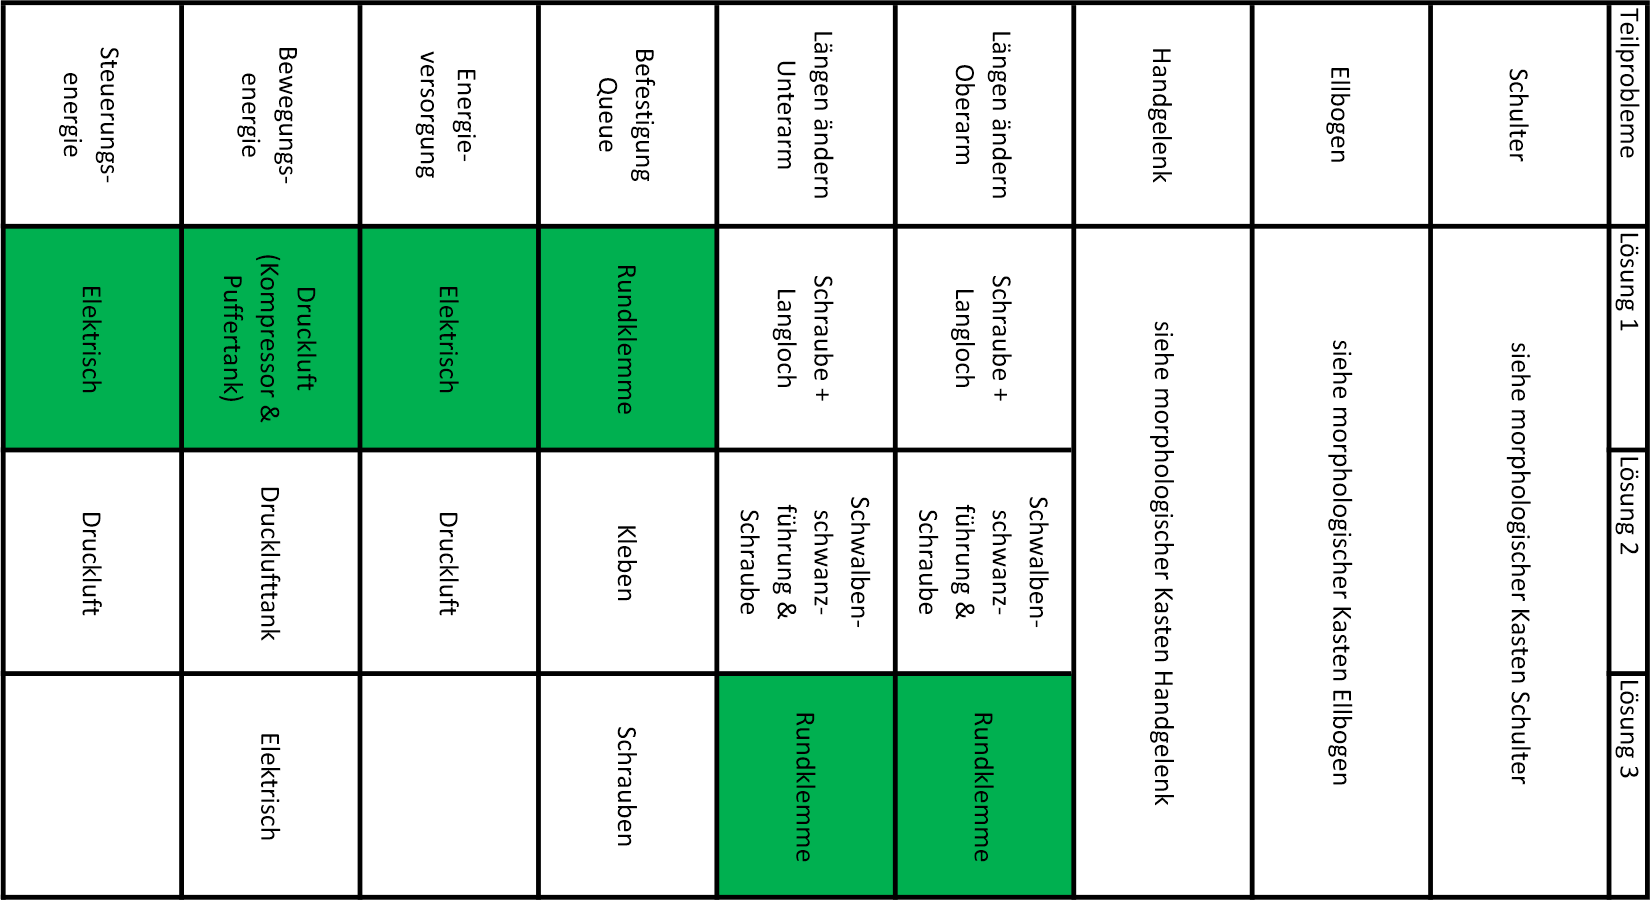
\includegraphics[angle=90, width=.8\textwidth]{Abb/MorphoBoxes/Morphologischer_Kasten_Teilprobleme.png}\label{tab:morphologische-kasten-teilprobleme}
			\end{table}
%
			\begin{table}[h]
				\centering
				\caption[Morphologischer Kasten der Schulter]{Morphologischer Kasten der Schulter.}
				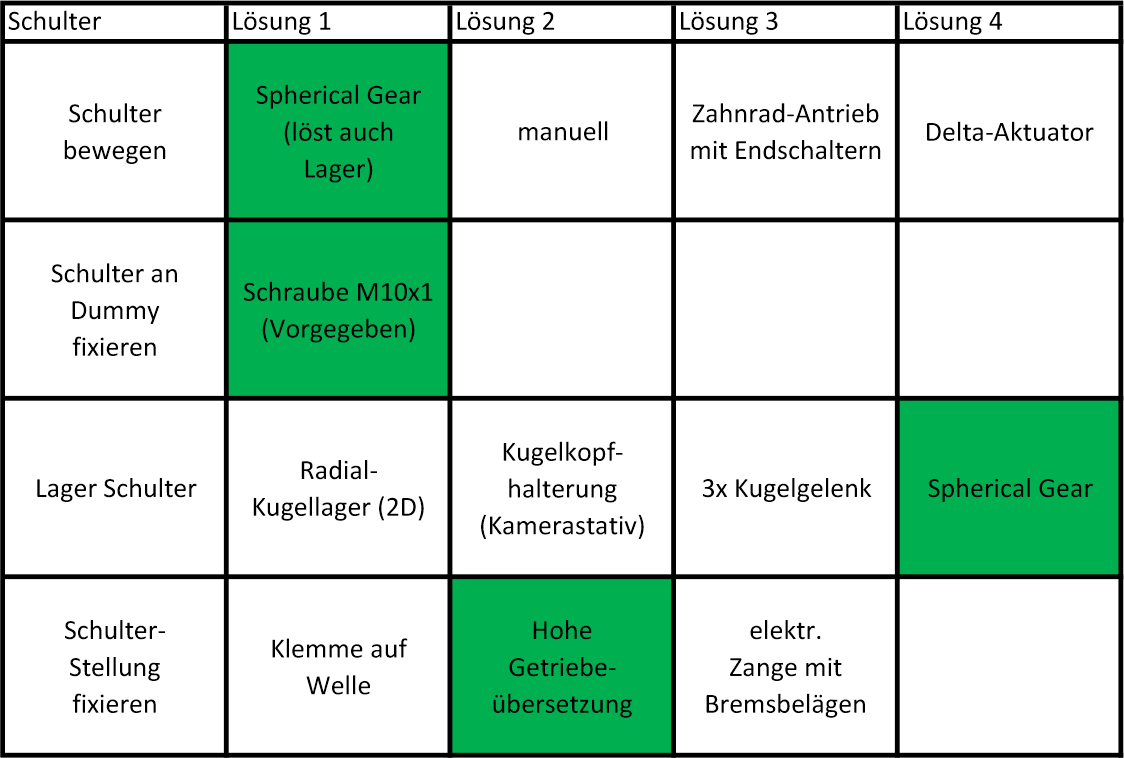
\includegraphics[width=.8\textwidth]{Abb/MorphoBoxes/Morphologischer_Kasten_Schulter.png}\label{tab:morphologische-kasten-schulter}
			\end{table}
%
			\begin{table}[h]
				\centering
				\caption[Morphologischer Kasten des Ellbogens]{Morphologischer Kasten des Ellbogens.}
				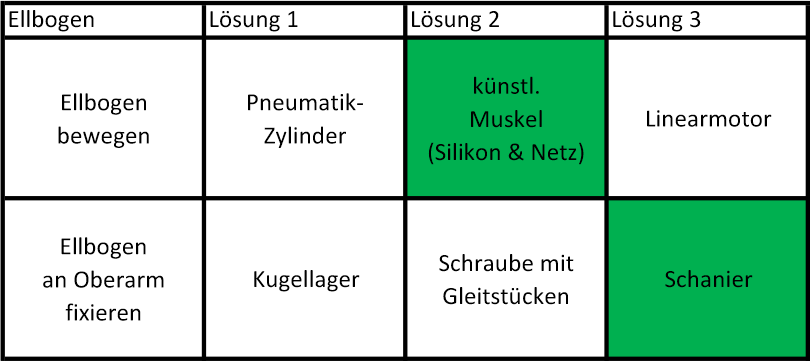
\includegraphics[width=.8\textwidth]{Abb/MorphoBoxes/Morphologischer_Kasten_Ellbogen.png}\label{tab:morphologische-kasten-ellbogen}
			\end{table}
%
			\begin{table}[h]
				\centering
				\caption[Morphologischer Kasten des Handgelenks]{Morphologischer Kasten des Handgelenks.}
				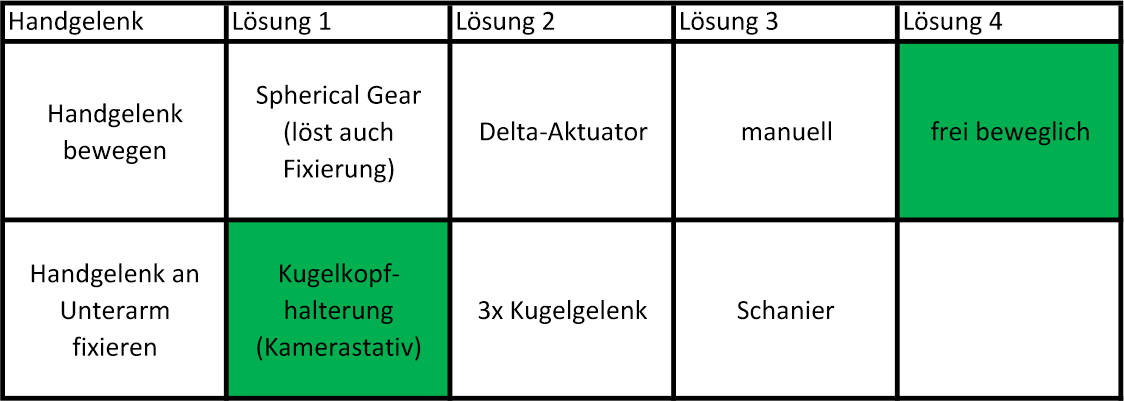
\includegraphics[width=.8\textwidth]{Abb/MorphoBoxes/Morphologischer_Kasten_Handgelenk.png}\label{tab:morphologische-kasten-handgelenk}
			\end{table}
%
			\begin{table}[h]
				\centering
				\caption[Morphologischer Kasten des Feedback-Systems]{Morphologischer Kasten des Feedback-Systems.}
				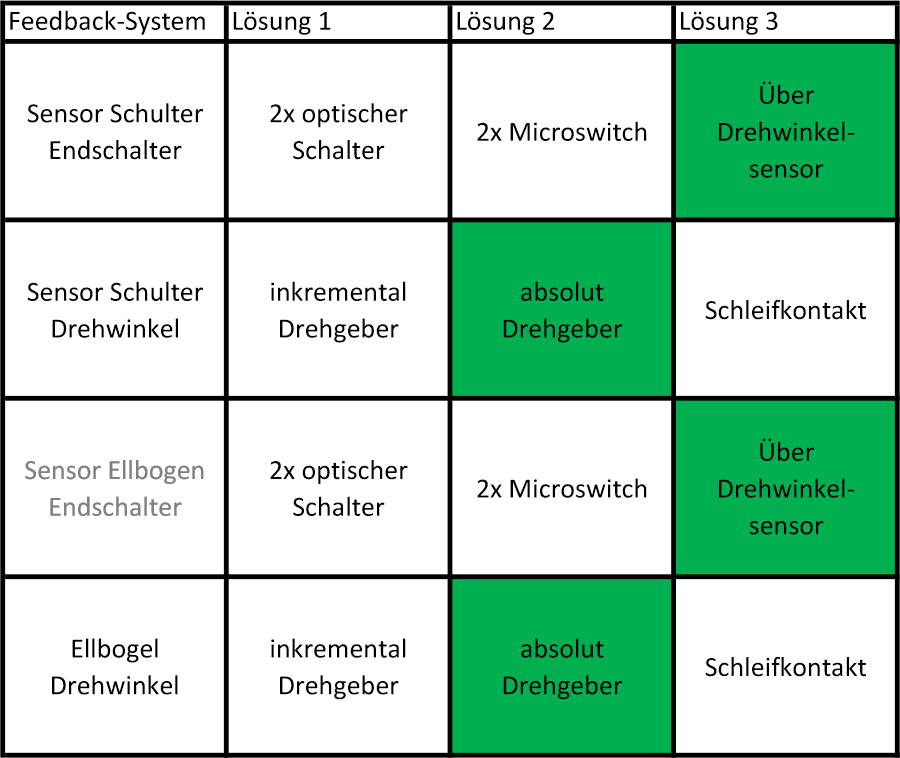
\includegraphics[width=.8\textwidth]{Abb/MorphoBoxes/Morphologischer_Kasten_Feedback-System.png}\label{tab:morphologische-kasten-feedback-system}
			\end{table}

		\subsection{Prinzipskizze}
			Da die Funktionen nun definiert sind, kann das Prinzip des Gerätes schematisch in einer Prinzipskizze aufgezeigt werden.\\
			Sie dient dazu, zu konstruierende Zusammenhänge zu verdeutlichen und bietet eine erste grobe Vorstellung des Geräts. Die bildliche Darstellung hilft außerdem die gewählten Lösungen aus den morphologischen Kästen im vorangegangenen Abschnitt zu verstehen.\\
			\Cref{fig:prinzipskizze-gesamtansicht} zeigt die Hauptbauteile, \cref{fig:prinzipskizze-ellbogen} den Anschluss zwischen Ober- und Unterarm und \cref{fig:prinzipskizze-handgelenk-und-hand} die Hand und ihre Verbindung zum Unterarm.

			\begin{figure}[h]
				\centering
				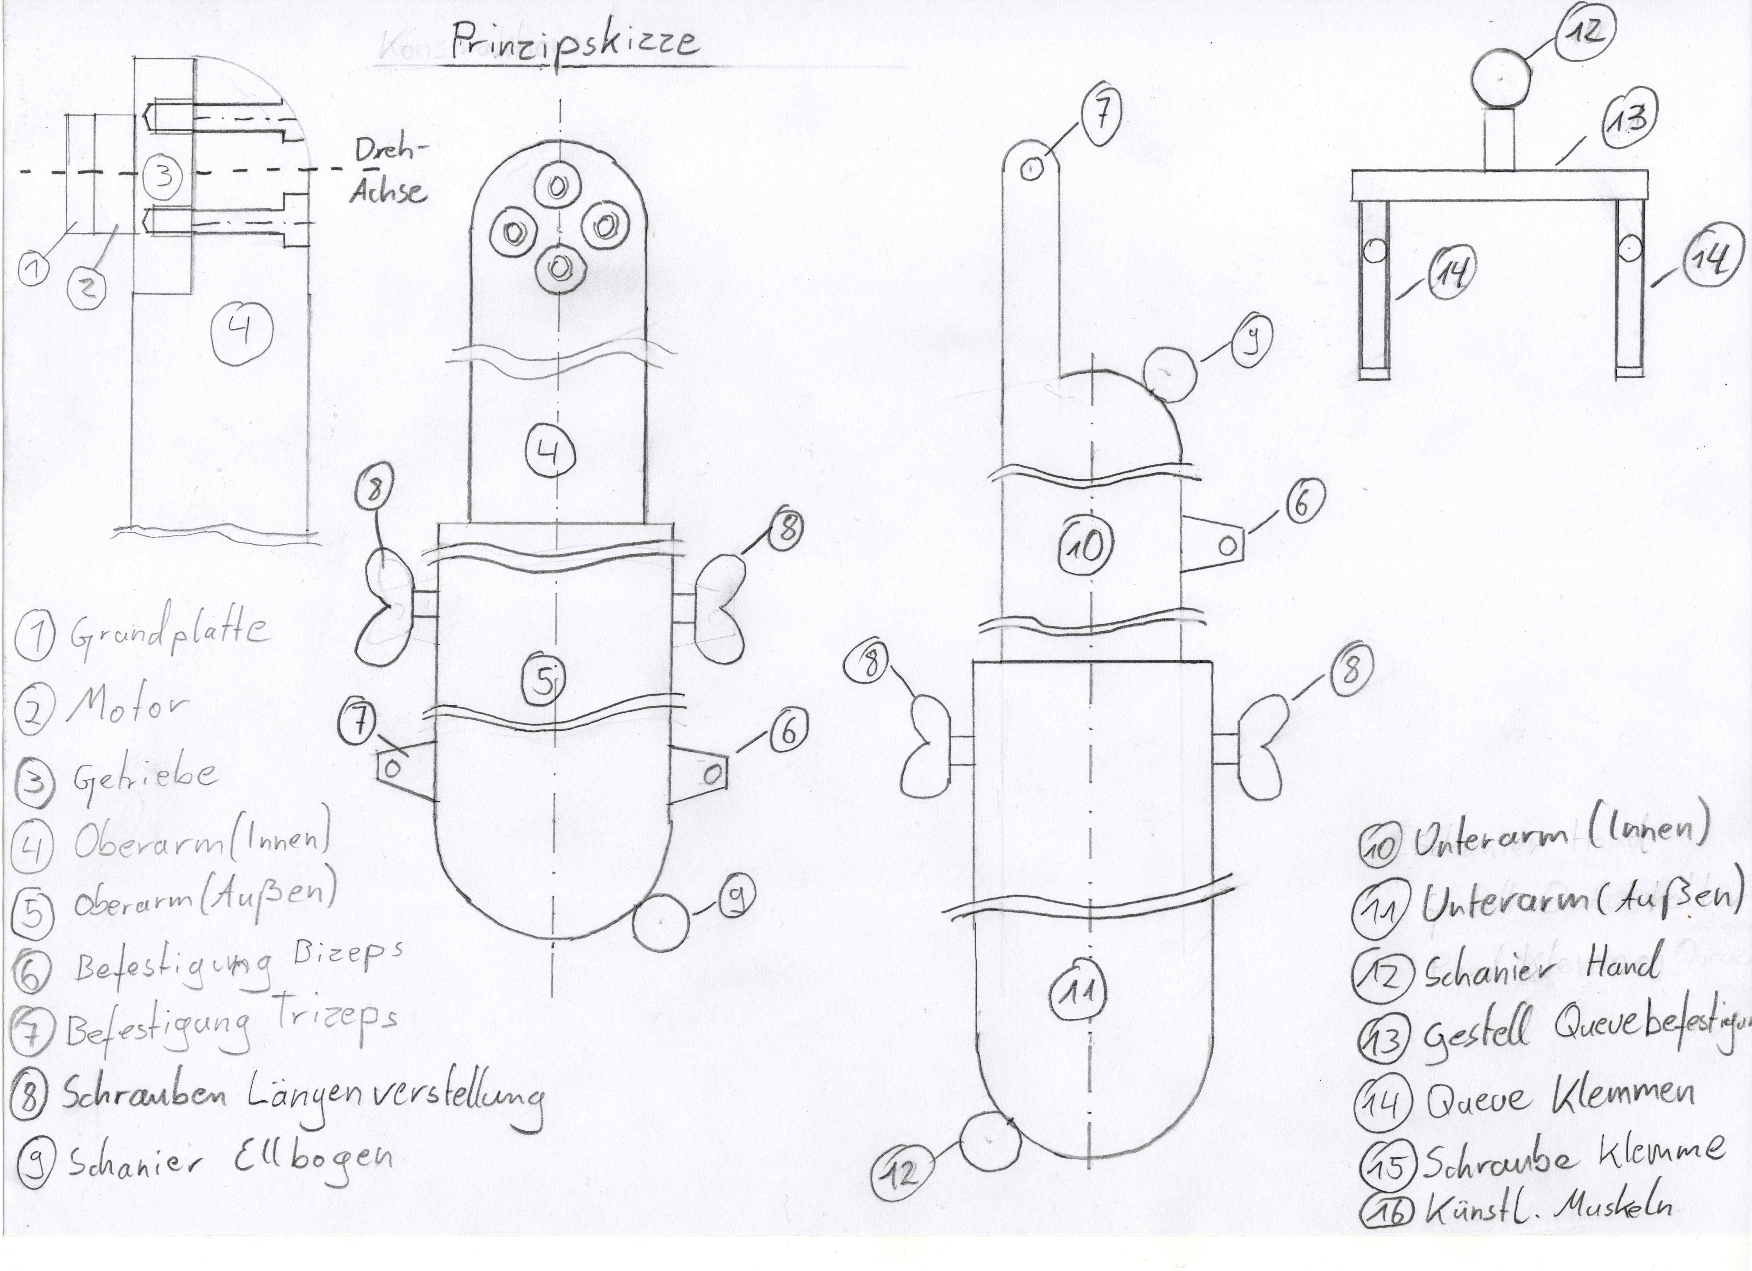
\includegraphics[width=\textwidth]{Abb/Prinzipskizze_Gesamtansicht}
				\caption[Prinzipskizze -- Gesamtansicht]{Prinzipskizze -- Gesamtansicht.}\label{fig:prinzipskizze-gesamtansicht}
			\end{figure}

			\begin{figure}[h]
				\centering
				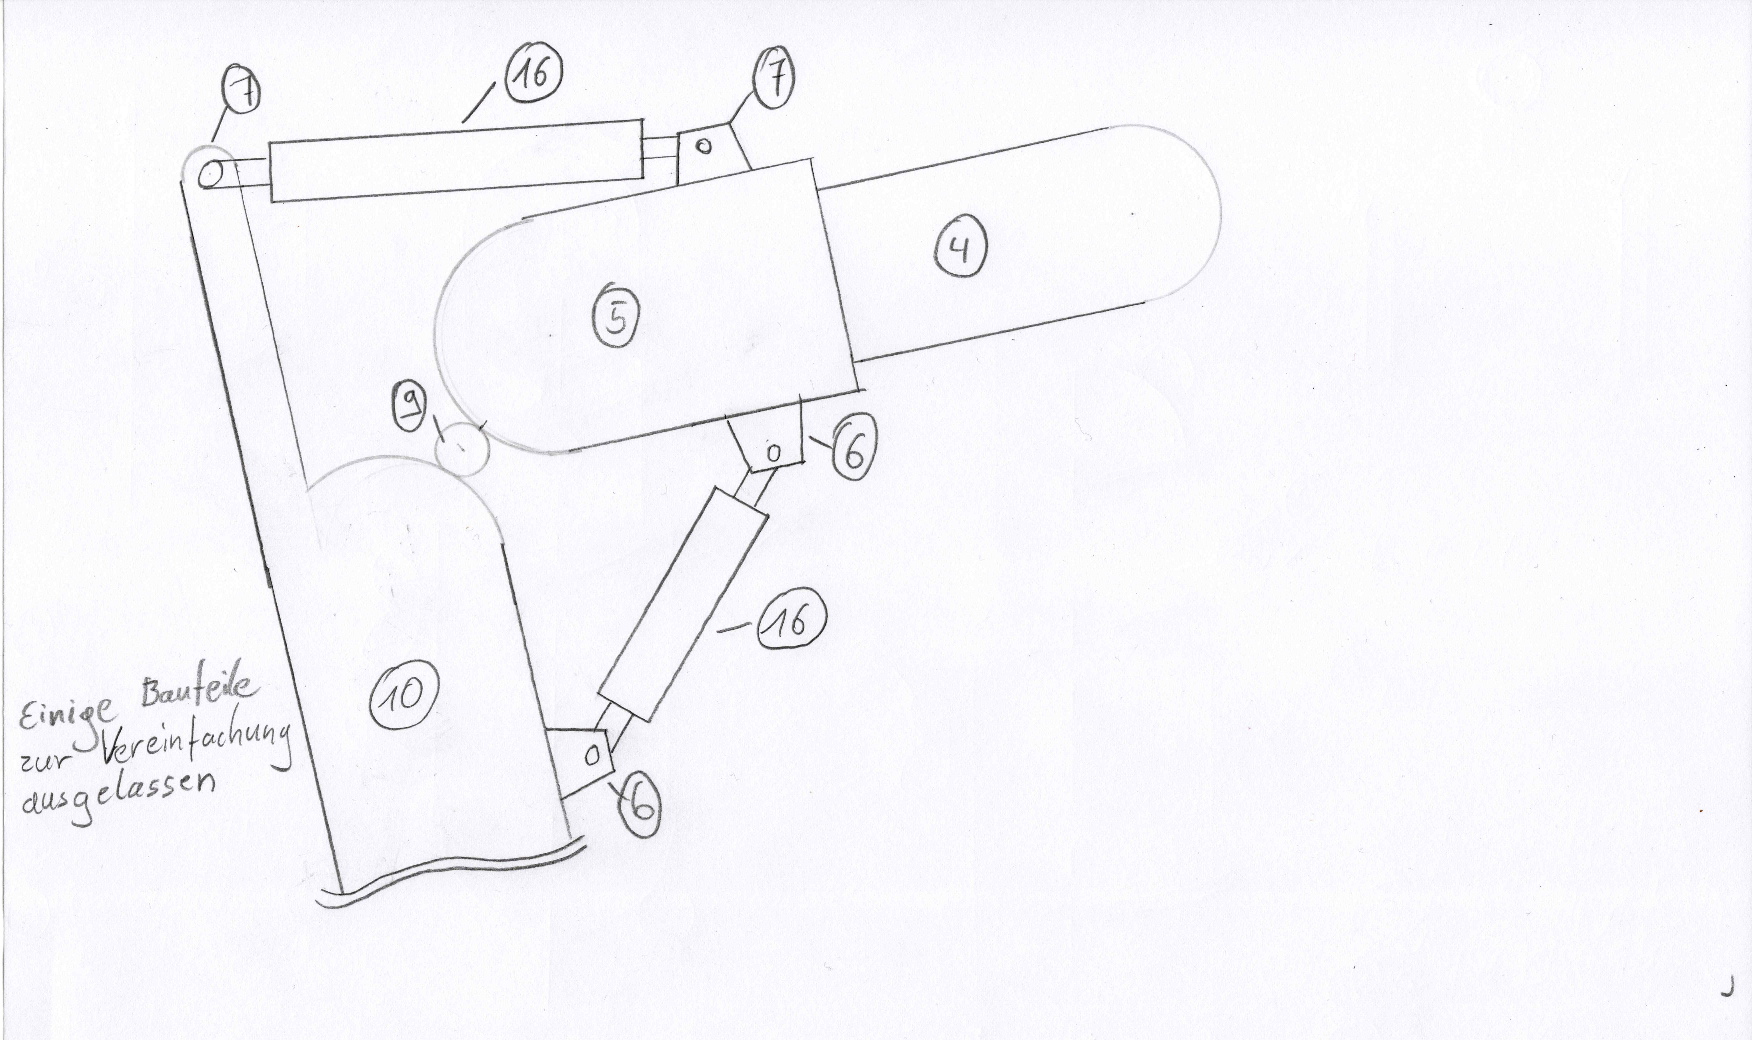
\includegraphics[width=\textwidth]{Abb/Prinzipskizze_Ellbogen}
				\caption[Prinzipskizze -- Ellbogen]{Prinzipskizze -- Ellbogen.}\label{fig:prinzipskizze-ellbogen}
			\end{figure}

			\begin{figure}[h]
				\centering
				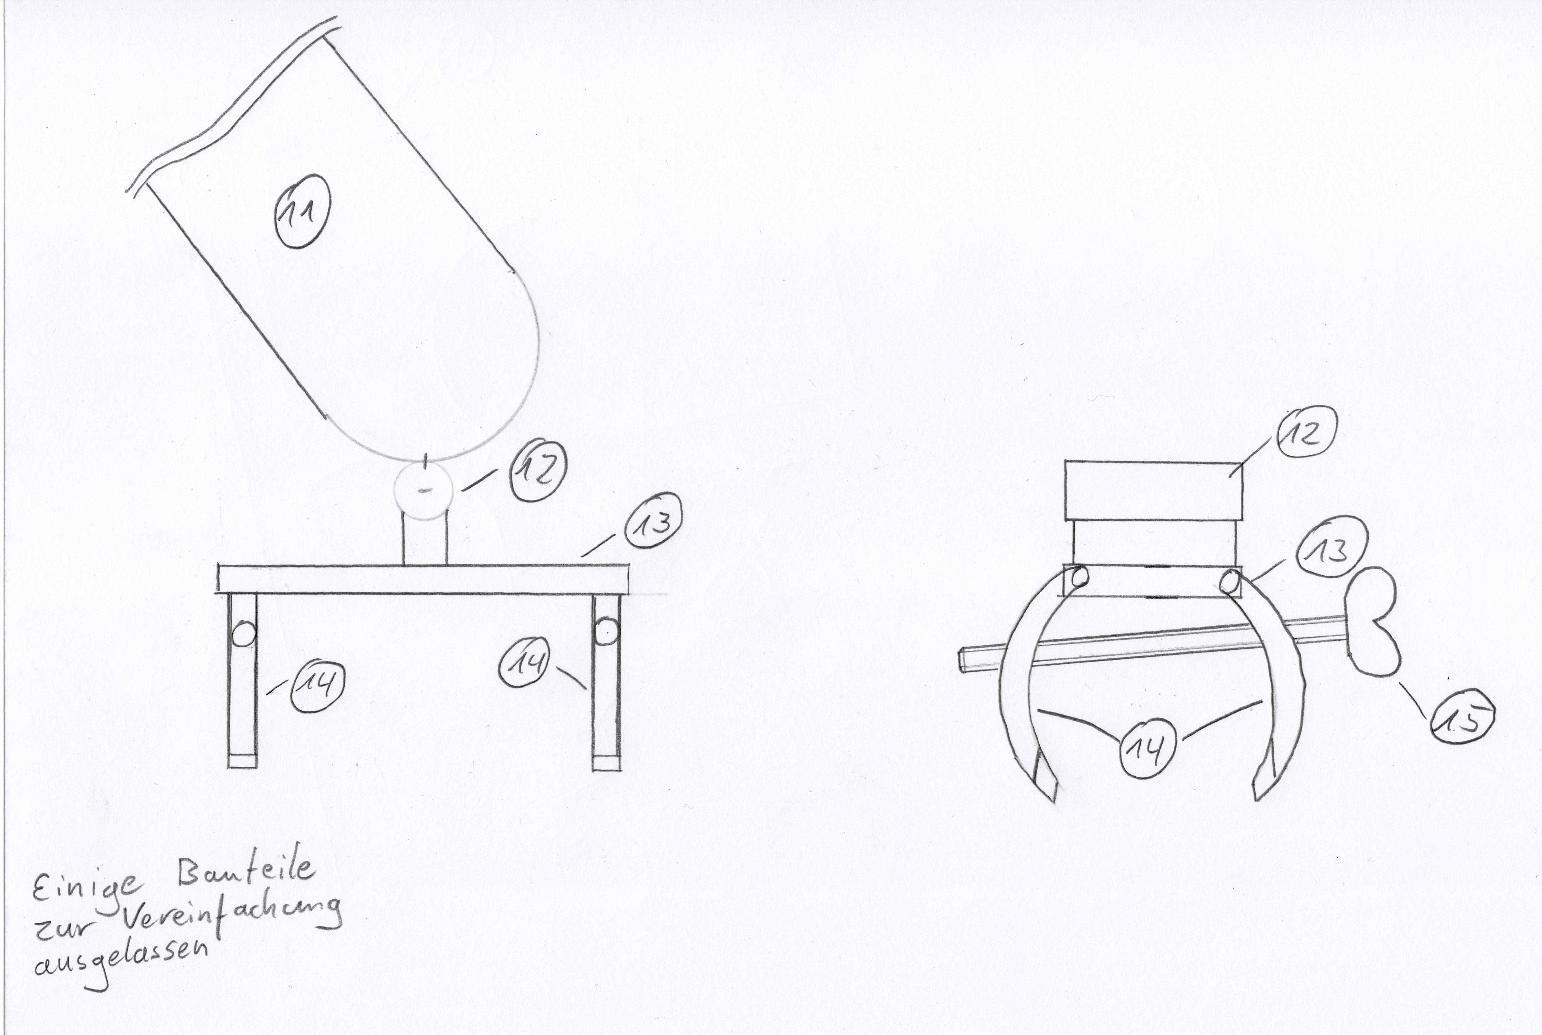
\includegraphics[width=\textwidth]{Abb/Prinzipskizze_Handgelenk_und_Hand}
				\caption[Prinzipskizze -- Handgelenk und Hand]{Prinzipskizze -- Handgelenk und Hand.}\label{fig:prinzipskizze-handgelenk-und-hand}
			\end{figure}

	\section{Begründung der Lösungsauswahl}\label{Begruendung Loesungsauswahl}

		Nun soll erläutert und erklärt werden, wieso die jeweiligen Lösungen aus den morphologischen Kästen ausgewählt wurden.\par\medskip

		Zunächst betrachten wir die übergeordneten Teilprobleme. Dazu zählt unter anderem die Einstellbarkeit der Armlängen. Diese sollen möglichst genau die Anatomie unterschiedlicher Menschen nachbilden. Um dies zu gewährleisten, müssen sie in der Länge verstellt werden können. Die passendste Lösung stellte dabei eine gewöhnliche Fahrradrohrklemme dar. Denn dazu muss nicht zusätzlicher Konstruktionsaufwand betrieben werden, sondern sie können zugekauft werden. Des Weiteren ist an dem Bauteil des Arms wenig Bearbeitungsaufwand. Diese bestehen aus Rohren und können einfach eingeschlitzt werden, um die Verklemmung der Fahrradklemmen auf das innen liegende Rohr zu übertragen. Die Auswahl für die Anpassungsmöglichkeit der Längen ist beim Oberarm und Unterarm identisch.\par\medskip

		Der nächste wichtige Punkt stellt die Befestigung des Queues dar. Dabei muss die Bewegung des Arms auf den Queue übertragen werden. Allerdings darf er sich nicht drehen, da es zu einer ungewollten Bewegung der Kugel führen könnte. Um dies zu gewährleisten, wurde eine Rundklemme gewählt. Sie umschließt den Queue am Griff und ist auch käuflich zu erwerben. Des Weiteren ist sie, anders als die anderen Möglichkeiten, nicht destruktiv.\par\medskip
		
		Die Energieversorgung des gesamten Aufbaus erfolgt mittels elektrischer Energie. Diese ist am einfachsten in andere Energien umzuwandeln und eigentlich überall verfügbar.\par\medskip
		Die Bewegungsenergie bzw. die Energie, die für den Stoß verwendet wird, wird über Druckluft bereitgestellt. Dabei wird sie mit einem mobilen Kompressor erzeugt und in einem Pufferspeicher zwischengespeichert. Sobald der Stoß ausgeführt werden soll, kann die gespeicherte Druckluft kontrolliert abgelassen werden. Bei der Lösung mit nur einem Drucklufttank ist der Nachteil, dass nur so lange Stöße ausgeführt werden können, solange genug Druckluft vorhanden ist. Ist der Tank einmal leer, muss er über einen Druckluftkompressor, die in Billardhallen üblicherweise nicht vorhanden sind, aufgefüllt werden.\par\medskip
		
		Die Steuerungsenergie wird ebenfalls als elektrische Energie bereitgestellt, da damit die Möglichkeit der Ansteuerung von Motoren, sowie das Feedback von Sensoren ermöglicht wird. Eine Steuerung über Pneumatik wäre ebenfalls möglich, allerdings bietet sie nicht die oben genannten Vorteile (vgl. \cref{tab:morphologische-kasten-teilprobleme}).\par\medskip
		
		Wie weiter oben schon erwähnt, wurden einige Bereiche in eigenen morphologischen Kästen aufgearbeitet. Darunter die Schulter, der Ellbogen und das Handgelenk. Diese werden im Folgenden vorgestellt.\par\medskip

		Das erste Teilproblem der Schulter stellte die Befestigung dieser und damit der gesamten Baugruppe an dem bereitgestellten Dummy dar. Allerdings ist der einzige Kontaktpunkt des Dummys eine Schraube mit dem Gewinde M10 $\times$ 1. Diese Lösung ist also von den Gegebenheiten vorgegeben.\par\medskip

		Um einen typischen Billardstoß nachbilden zu können, muss sich außerdem die Schulter bewegen können, da der Arm eines Billardspielers meistens einen Winkel von \SI{90}{\degree} gegenüber der Senkrechten bildet. Da dieser Winkel jedoch von Spieler zu Spieler unterschiedlich ist, musste die Schulter beweglich ausgeführt werden. Um die Bewegung der Schulter umzusetzen, wurde ein spherical gear gewählt, da dies neben der eigentlichen Bewegung auch die Lagerung der Schulter als auch die Fixierung, während eines Stoßes sicherstellt, indem die Getriebeübersetzung entsprechend hoch gewählt wird. Da mit dieser Lösung mehrere Probleme auf einmal gelöst werden können und sie einen relativ kleinen Bauraum einnimmt, wurde diese Variante ausgewählt. Dabei wird allerdings die Bewegung der Schulter auf eine 2D-Ebene beschränkt, was aber für die Nachbildung eines Arms beim Billardspielen keinen Nachteil mit sich bringt (vgl. \cref{tab:morphologische-kasten-schulter}).\par\medskip

		Außerdem muss eine Bewegung am Ellbogen erzeugt werden, da damit die meisten Billardspieler ihren Stoß ausführen. Dabei gab es zwei Probleme zu lösen: Zum einen die Bewegung und zum anderen die Befestigung des Unterarms am Oberarm. Zur Bewegung des Unterarms wurden künstliche Muskeln gewählt. Sie sind flexibel und bilden die menschliche Anatomie sehr genau nach. Um die Bewegung des Arms zu ermöglichen, wurde ein gewöhnliches Scharnier gewählt, da auch dies den Konstruktionsaufwand gering hält und hinzugekauft werden kann (vgl. \cref{tab:morphologische-kasten-ellbogen}).\par\medskip

		Als letztes Problem wird das Handgelenk betrachtet. Dieses muss sich einerseits bewegen und andererseits am Unterarm befestigt werden. Da vom Handgelenk aber bei einer Lagerung des Queues keine eigene Bewegung erforderlich ist wurde die Hand so aufgelegt, dass sie nicht maschinell bewegt werden kann. Als Fixierung und Lagerung wurde am Handgelenk ein 3D-Kugelkopf gewählt, da damit eine genauere Positionierung des Queues möglich ist. So kann er auch in einem Winkel zum Arm ausgerichtet werden und bietet mehr Flexibilität bei der Nachstellung von Stößen (vgl. \cref{tab:morphologische-kasten-handgelenk}).
	\section{Auslegung der Schulter}\label{sec:auslegung}

		\begin{figure}[h]
			\centering
			\includesvg[inkscapelatex=true, width=.6\textwidth]{Abb/schulterauslegung}
			\caption[Vereinfachtes Modell des Systems Schulter-Oberarm-Unterarm]{Vereinfachtes Modell des Systems Schulter-Oberarm-Unterarm mit den Massen \(m_o, m_u\), den Längen \(l_o, l_u\) und dem verursachten Drehmoment \(M_m\).}%
			\label{fig:modell schulter oberarm unterarm}
		\end{figure}
		
		Nach \cite{Soll.1982} entfallen anteilig des Gesamtkörpergewichtes etwa \SI{3}{\percent} auf den Oberarm und \SI{2}{\percent} auf den Unterarm.
		Mit einem angenommenen Gesamtkörpergewicht von \SI{80}{\kilo\gram} entspricht das einem Massenanteil von \SI{2,4}{\kilo\gram} auf den Oberarm und \SI{1,6}{\kilo\gram} auf den Unterarm.
		Hier soll von einer homogenen Massenverteilung ausgegangen werden, womit die jeweiligen Massenschwerpunkte mittig auf der Verbindungslinie zwischen den Gelenken liegt.
		Weiter wird von jeweiligen Längen für Ober- und Unterarm von \SI{0,35}{\metre} und einer Masse \(m_q\) am Ende des Unterarms von \SI{0,5}{\kilo\gram} ausgegangen.\par
		Soll beim Stoß der Oberarm horizontal und der Unterarm orthogonal nach unten gerichtet sein, so befindet sich das Gesamtgewicht des Systems mit \SI{4}{\kilo\gram} entlang der Oberarmachse nach \cref{eq:massenschwerpunkt arme} bei \SI{0,257}{\metre}.

		\begin{align}
			x_s &= \frac{\frac{1}{2}l_o \cdot m_o + l_o \cdot \left(m_u + m_q\right)}{m_o + m_u + m_q} \nonumber \\
				&= \frac{\SI{0,175}{\metre} \cdot \SI{2,4}{\kilo\gram} + \SI{0,35}{\metre} \cdot \left(\SI{1,6}{\kilo\gram} + \SI{0,5}{\kilo\gram}\right)}{\SI{4,5}{\kilo\gram}} \nonumber \\
				&\approx \SI{0,257}{\metre}%
				\label{eq:massenschwerpunkt arme}
		\end{align}

		Um eine stabile Orientierung des Oberarms um das Schultergelenk gewährleisten zu können muss so ein Drehmoment von mindestens \(M_m = x_s \cdot \left(m_o + m_u + m_q\right) = \SI{1,157}{\newton\metre}\) erzeugt werden können.
		Vergleich mit den Kenndaten eines Schrittmotors der Baugröße Nema 23 \cite{nanotec.specs} kann hier im Vollschrittbetrieb ein Haltemoment von \SI{2,95}{\newton\metre} erwartet werden.\par\medskip
		Die genannten Winkelauflösung des Schrittmotors von \SI{1,8}{\degree} übersetzt sich an der Position der Hand zu einer Mindestbogenlänge von
		\begin{align}
			\Delta s_{arc} 	&= \frac{\SI{1,8}{\degree}}{\SI{180}{\degree}} \cdot \pi \cdot l_{eff} = \frac{\SI{1,8}{\degree}}{\SI{180}{\degree}} \cdot \pi \cdot \sqrt{2 \cdot \left(\SI{0,35}{\metre}\right)^2} \nonumber \\
							&= \SI{1,56}{\cm}
		\end{align}
		Hier sei \(l_{eff}\), wie in \cref{fig:schultergelenk winkelaufloesung} dargestellt, die Hypotenuse des durch Ober- und Unterarm aufgespannten Dreieckes.\par
		Da mit nicht-idealen Steifigkeiten der Teilsysteme zu rechnen ist und um Abweichungen durch dynamisches Verhalten im Betrieb auffangen zu können wird ein Untersetzuingsverhältnis
		Die verfahrbare Mindestbahnlänge \(\Delta s_{arc}\) skaliert umgekehrt proportional mit dem Untersetzungsverhältnis \(N\) aus \cref{eq:untersetzung} gemäß
		\begin{equation}
			\Delta s_{arc} 	&= \frac{1}{N} \cdot \frac{\SI{1,8}{\degree}}{\SI{180}{\degree}} \cdot \pi \cdot l_{eff}
		\end{equation}

		\begin{figure}[h]
			\centering
			\includesvg[inkscapelatex=true, width=.6\textwidth]{Abb/schulterauslegung-winkelaufloesung}
			\caption[Die effektive Länge \(l_{eff}\) zwischen Drehachse des Schultergelenks und der Hand]{Die effektive Länge \(l_{eff}\) zwischen Drehachse des Schultergelenks und der Hand (aufhängung des Queues) entspricht hier der Hypotenuse des von Ober- und Unterarm aufgespannten Dreieckes.}%
			\label{fig:schultergelenk winkelaufloesung}
		\end{figure}
	\section{Auslegung der künstlichen Muskeln}
		Es erfolgt die Berechnung der benötigten Kraft, die der Bizeps aufbringen muss, um die Kugel mit der entsprechenden Geschwindigkeit stoßen zu können. 
		Dazu wurde in eigener Recherche ermittelt, dass die maximalen Geschwindigkeiten \(v_{Kugel}\) einer Billardkugel bei ungefähr \SI{40}{\kilo\metre\per\hour}, also \SI{11,1}{\metre\per\second}, liegt.
		Die Gewichte der Kugeln wurde aus der Aufgabenstellung entnommen, dabei wurde die größte Masse angenommen, um alle Arten an Kugeln mindestens mit einer Geschwindigkeit von \SI{11,1}{\metre\per\second} bewegen zu können.
		Diese Masse beträgt \(m_{Kugel}\) = \SI{204}{\gram}.
		Die Masse des Arms \(m_{Arm}\) wurde mithilfe des CAD-Programms \textsc{Solidworks} ermittelt. Sie liegt bei \SI{1,1}{\kilo\gram}.
		Wichtig dabei ist, dass es sich lediglich um die Masse handelt, die bei einem Stoß bewegt wird. 
		Mit diesen Angaben lässt sich nun nach \cref{eq:SollgeschwindikeitArm} die Geschwindigkeit, mit der der Arm bewegt werden muss ermitteln. 

		\begin{equation}
			v= \frac{\SI{0,204}{\kilogram} \cdot \SI{11,1}{\metre\per\second}}{\SI{1,105}{\kilogram}} = \SI{2,05}{\metre\per\second}
			\label{eq:SollgeschwindikeitArmZahlen}
		\end{equation}
		Die Massen, Massenschwerpunkte und die Längen, die für die Berechnung der Kraft benötigt wurden, werden ebenfalls mithilfe von SolidWorks ermittelt. 
		Zur Ermittlung der Kraft wird die \cref{eq:Kraft-PAM} verwendet. 

		\begin{equation}
			F =\frac{\SI{1,105}{\kilogram} \cdot \SI{17867,67}{\milli\metre\squared} \cdot \SI{420}{\metre\per\second\squared}}{\SI{304,29}{\milli\metre} \cdot \SI{136,35}{\milli\metre} \cdot \cos{\SI{46,38}{\degree}}} = \SI{289,72}{\newton}
		\end{equation}
		mit \(a_T\)
		\begin{equation}
			a_T = \frac{\SI{4,2}{\metre\squared\per\second\squared}}{\SI{10}{\milli\metre}} = \SI{420}{\metre\per\second\squared}
		\end{equation}
		
		So ergibt sich eine minimal benötige Kraft der künstlichen Muskeln von \SI{289,72}{\newton}.
% \layout%
% Dieses Kapitel bildet zusammen mit dem folgenden Kapitel Diskussion den Hauptteil der Arbeit. In übersichtlicher Gliederung und sinnvoller Reihenfolge wird dargestellt, was mittels der eingesetzten Methodik im Hinblick auf die Zielsetzung herausgefunden werden konnte. Die Strukturierung des Kapitels orientiert sich an der Theorie und Methodik. Mit Hilfe von Grafiken und Diagrammen (siehe 2.8.4) werden die Ergebnisse wertfrei dargestellt. Eine Interpretation erfolgt an dieser Stelle noch nicht.
\chapter{Ergebnisse}
	Das auf Basis der vorangegangenen Überlegungen entwickelte Gerät soll in den folgenden Kapiteln anhand technischer Zeichnungen näher erläutert werden.
	Eine vollständige technische Dokumentation ist in \cref{sec:zeichnungen} zu finden.
	\section{Konzeption und Entwurf}
		Nun werden die zur Konstruktion konzipierten Bauteile allesamt mit Zeichnungen präsentiert und kommentiert.
		Dabei wird unter anderem sowohl auf das Prozedere der Konstruktion als auch auf die aufgetauchten Probleme und die Vorgehensweise zur Lösung jener eingegangen.\\
		Die technischen Zeichnungen zu den Bauteilen sind jeweils in \cref{zeichnungen} angehängt.
		Die Übersichtszeichnungen sind meist explosionsartige Darstellungsformen und enthalten Nummerierungen, die dann jeweils in der darauffolgenden Stückliste manifestiert sind.\\
		Die Zeichnungen zu dem Gesamtbauteil befinden sich in \cref{bauteilzeichnungen}, die des Schultergelenks in \cref{zeichnungen-schulter}, die Einzelteile des Ober-/Unterarms in \Cref{zeichnungen-arme} und die des Ellbogengelenks in \cref{zeichnungen-ellbogen}.
		Zu dem befinden sich in \cref{stuckliste-pneumatik} weitere sonstige Stücklisten und außerdem der Schaltplan für die Pneumatik.
		
	\section{Gesamtbauteil}
		Wie vorhin bereits erwähnt, sind die Zeichnungen des Gesamtbauteils im \cref{bauteilzeichnungen} angehängt.
		Diese zeigen das fertige Konstrukt als Ganzes und auseinander geschraubt.
		Die Maße und Dimensionierungen der Einzelteile sind den Zeichnungen der jeweilig zugehörigen Unterkapiteln zu entnehmen.\\
		Allgemein ist zu sagen, dass die Bauteile so konstruiert werden mussten, dass sie einander angepasst sind.
		Dabei spielen die Verbindungen zwischen den einzelnen Gliedern eine entscheidende Rolle.
		Das Gesamtbauteil besteht aus Schulter, Oberarm, Muskeln (Bizeps/Trizeps), Ellbogen, Unterarm und Hand.
	
	\section{Schulter}
		Die Schulter hat die Aufgabe sowohl den gesamten Arm am Dummy zu befestigen als auch die Bewegung des Arms zu initialisieren.
		Für diese Aufgabe wurde das Zykloidalgetriebe gewählt und konstruiert.
		Das Zykloidalgetriebe ist ein mechanisches Getriebe, das die Umdrehungen reduziert, indem es die exzentrische Bewegung des Zykloidenrads einstellt, welches die Ausgangswelle antreibt. Es besitzt ein hohes Übersetzungsverhältnis und ist somit gut geeignet für unsere Anwendung.
		Das Schultergelenk ist ebenfalls in \cref{bauteilzeichnungen} und weitere Einzelheiten in \cref{zeichnungen-schulter} zu betrachten.
	
	\section{Ellbogen}
		Der Ellbogen fungiert als Verbindung von Ober- und Unterarm und als Halterung- bzw. Stützpunkt des Trizeps.
		Er ist unter \cref{bauteilzeichnungen} genauer anzusehen.
		Das Ellbogengelenk ist mit gekauften und gedruckten Teilen erstellt.
		Dabei werden alle Teile, die käuflich erworben werden können, auch zugekauft.
		Die selbst konstruierten Einzelteile wie das Rohrteil ist in \cref{zeichnungen-ellbogen} zu sehen.
	
	\section{Ober-/Unterarm}
		Die Konstruktion des Ober- und Unterarms wurde zunächst an den Prinzipskizzen orientiert erstellt.
		Dazu wurden entsprechende Bauteile in CAD gezeichnet und als Baugruppe zusammengefügt.
		Allerdings zeigte sich nach ersten Berechnungen zu den künstlichen Muskeln, dass diese Konstruktion deutlich zu schwer war, um sie mit der Kraft der künstlichen Muskeln zu bewegen.
		Nach weiteren Recherchen wurde außerdem klar, dass die Bauteile einen extrem hohen Preis in der Fertigung auswiesen.
		Aus diesen Gründen musste nach kurzer Zeit die Konstruktion komplett überarbeitet werden.
		Dabei wurde besonders darauf geachtet, dass sich sowohl das Gewicht möglichst gering hält als auch die Kosten durch die Verwendung von Kaufteilen reduzieren.
		Dies führte dazu, dass die Konstruktion nahezu komplett aus Aluminiumrohren und 3D-gedruckten Teilen konstruiert wurde.
		Dabei liegt auch der Vorteil, dass nicht alle Bauteile eigenständig konstruiert werden müssen.
		So lassen sich zum Beispiel die Klemmen, die die Rohrteile miteinander verbinden, als gewöhnliche Fahrradklemmen ausführen.
		Auch die Anschlüsse der künstlichen Muskeln können als 3D-gedruckte Teile ausgearbeitet werden und mit einer einfachen Rohrschelle an die Arme befestigt werden.
		Spezielle Teile wie die Einsätze der Rohre wurden eigenständig konstruiert.\\
		Der Ober- und Unterarm als Ganzes ist in \cref{bauteilzeichnungen} zu sehen und die Einzelteile wie die Innen- und Außenrohre sind in \cref{zeichnungen-arme} zu betrachten.
	
	\section{Hand}
		Das Handgelenk sowie die Hand (abgebildet in \cref{bauteilzeichnungen}) bestehen im Wesentlichen aus gekauften Teilen.
		Dabei wird das Handgelenk so ausgelegt, dass es sowohl mit einer Klemme mit einer Kugelform als Anschluss ausgestattet werden kann als auch mit einer Schraube der Größe M5 befestigt werden kann.
		Dabei ist lediglich zu beachten, dass die Kugelform mit einem Durchmesser von 28 mm ausgeführt ist.
		Die Klemme bzw. Hand sollte des Weiteren breit genug ausgearbeitet sein, um dem Queue auch eine entsprechende seitliche und vertikale Stabilisation zu ermöglichen.
	
	\section{Künstliche Muskeln}
		Die künstlichen Muskeln bilden hauptsächlich der Bizeps und der Trizeps, welche ebenso in \cref{bauteilzeichnungen} zu sehen sind.
		Beide sind jeweils mit einem Ende am Oberarm und mit dem anderen Ende am Unterarm verbunden.
		Die Muskeln funktionieren durch pneumatischen Antrieb.
		Diese Pneumatik verlangt eine Verschaltung, wie sie in \cref{stuckliste-pneumatik} schematisch dargestellt ist.
% In diesem Kapitel werden die Ergebnisse hinsichtlich der Problem- und Zielstellung ausgewertet und interpretiert. Die Bedeutung der Ergebnisse für die wissenschaftliche Diskussion und die Konsequenzen für die entsprechenden Praxisfelder sollte argumentiert werden. Die Kapitel Ergebnisse und Diskussion sollten in etwa zwei Drittel Ihrer Arbeit ausmachen.
\chapter{Diskussion}
	Nach der Präsentation der Konstruktionsergebnisse kann nun eine Auswertung über den Erfolg oder die Probleme erfolgen.
	Es sollen ebenfalls auf Aspekte der allgemeinen Vorgehensweise und der Gruppenarbeit eingegangen werden.\par \medskip
	Die gewählten Lösungen bringen alles mit sich, was sie in unserer Vorstellung versprachen.\\
	Das Schultergelenk hat mit dem Zykloidalgetriebe den mechanischen Ansprüchen genügt.
	Da bei dem Akt eines Billardstoßes die Schulter die Arme nur nach vorne und hinten bewegt, und sie nicht etwa nach außen klappt, ist die konstruierte Schulter dem eines echten Menschen beim Stoßen einer Kugel mittels eines Queues relativ nahe.\\
	Der Ober- und Unterarm sind der Ähnlichkeit eines menschlichen Körpers willen als zylindrische Rohre ausgeführt.
	Das bedeutet zugleich aber auch, dass die Form zum konstruieren unpraktischer ist, da in die Rohre auch Schlitze und Löcher eingesetzt werden müssen.
	Die Handhabung mit flachen, rechteckigen Bauteilen wären im Allgemeinen einfacher gewesen.
	Da dies jedoch kein größeres Problem darstellt, ist die ursprüngliche Option beibehalten.\\
	Ähnlich wie beim Schultergelenk sieht es auch mit dem Ellbogengelenk aus.
	Da das Gelenk nur die Aufgabe hat, Ober- und Unterarm miteinander zu verbinden, sie stabil zu halten und richtig auszulenken, genügt ein scharnierartiges Konstrukt den Anforderungen.
	Dadurch, dass bei der geforderten Bewegung der Unterarm nicht nach innen geklappt werden muss, ist der von uns konstruierte Ellbogen mit seiner Bewegungskoordination ausreichend.\\
	Was die Muskeln anbelangt, wurde bereits argumentiert, dass die Ausführung als künstliche Muskeln der menschlichen Anatomie und Physiologie sehr nahekommt und deshalb verwendet wurde.
	Viel einfacher, sowohl für die Konstruktion als auch für die Handhabung, wäre es gewesen, eine alternative Variante zu wählen.
	Dadurch, dass die Muskeln pneumatisch funktionieren, sind sie auch an einem dementsprechenden Antrieb gebunden, welches den Aufwand erhöht.
	Nach Abwägung und auf Wunsch des Kunden bzw. Auftragsgebers ist dennoch auf die künstlichen Muskeln zurückgegriffen worden.\\
	Die Hand schien wie erwartet den kleinsten konstruktiven Aufwand zu verlangen.
	Da sie nur die Aufgabe des Queuehalters hat und dies nicht viel erfordert, kann die Halterung als Kaufteil erworben werden.
	Dann bleibt nur noch das Handgelenk übrig.
	Das Handgelenk verbindet mit der ausgewählten Variante den Unterarm und die Hand beweglich, so dass keine ungewollten Verdrehungen oder Sonstiges auftreten.\par \medskip
	Da zum ganzen Konstruktionsprojekt ein Team in Form einer Dreiergruppe gehört, wird auch dieser Aspekt zur Bewertung herangezogen.\\
	Das Konstruktionsteam kennt sich untereinander relativ gut, weshalb Probleme und Unstimmigkeiten schnell ausdiskutiert werden konnten.
	Des Weiteren ist jedem klar, welches Repertoire jeweils die anderen besitzen, weshalb die Aufgabenverteilung mehr oder weniger vorbestimmt war.\\
	Es gab außerdem wöchentliche Meetings mit dem Auftragsgeber bzw. dem Veranstaltungsleiter, der zu jedem Schritt mit seiner Erfahrung und Expertise Ratschläge geben konnte, die der Gruppe sehr geholfen hat.
	Es konnten somit Fragen und Unklarheiten geklärt und weitere Schritte besprochen werden.\\
	Ein Problem war allerdings die unterschiedlich vielen Know-Hows der Teammitglieder.
	Dies führte dazu, dass an der einen oder anderen Stelle einige Ausarbeitungsideen nicht sofort nachvollzogen werden konnten.
	Eine unterschiedliche Verteilung der Arbeitslast auf die Individuen ließ sich deshalb nicht verhindern.

% Hier ist abschließend ein prägnanter Überblick über die Problemstellung, die Ergebnisse und deren Interpretation zu geben. Jede Arbeit hat bestimmte Beschränkungen und ungelöste Fragen. An dieser Stelle sollten die wesentlichen Grenzen der Untersuchung aufgezeigt werden. Aufgrund dieser Erkenntnisse sollte der/die VerfasserIn auch Hinweise auf zukünftige Arbeiten und mögliche Verbesserungen geben. Die Zusammenfassung sollte 2 A4-Seiten nicht überschreiten.
\chapter{Zusammenfassung}
	Die Problemstellung einen funktionierenden Arm zu entwerfen, der einen Billardstoß ausführen kann, wurde lange und durchdacht versucht zu lösen.
	Nun liegt eine Konstruktion vor, welche in Rahmen der Lehrveranstaltung "`Gerätekonstruktion"' so gut wie möglich ausgearbeitet wurde.\par \medskip
	Rückblickend ist zu sagen, dass bei der Konstruktion sehr viel Wert auf Funktionstüchtigkeit in verwirklichter Form gelegt wurde.
	Deshalb können wir guten Gewissens behaupten, dass das Ziel der Aufgaben- und Problemstellung erreicht wurde.\\
	Inwieweit die das Gerät in der Praxis funktioniert, ist noch eine offene Fragestellung.
	Dieser Frage könnte im Rahmen einer Projektarbeit beispielsweise nachgegangen werden.
%-----------------------------------------------------------------
\newpage
\listoffigures
\listoftables
\appendix
% \chapter{Zeichnungen}\label{sec:zeichnungen}
\newpage
\setlength{\voffset}{0cm}
\setlength{\hoffset}{0cm}
%
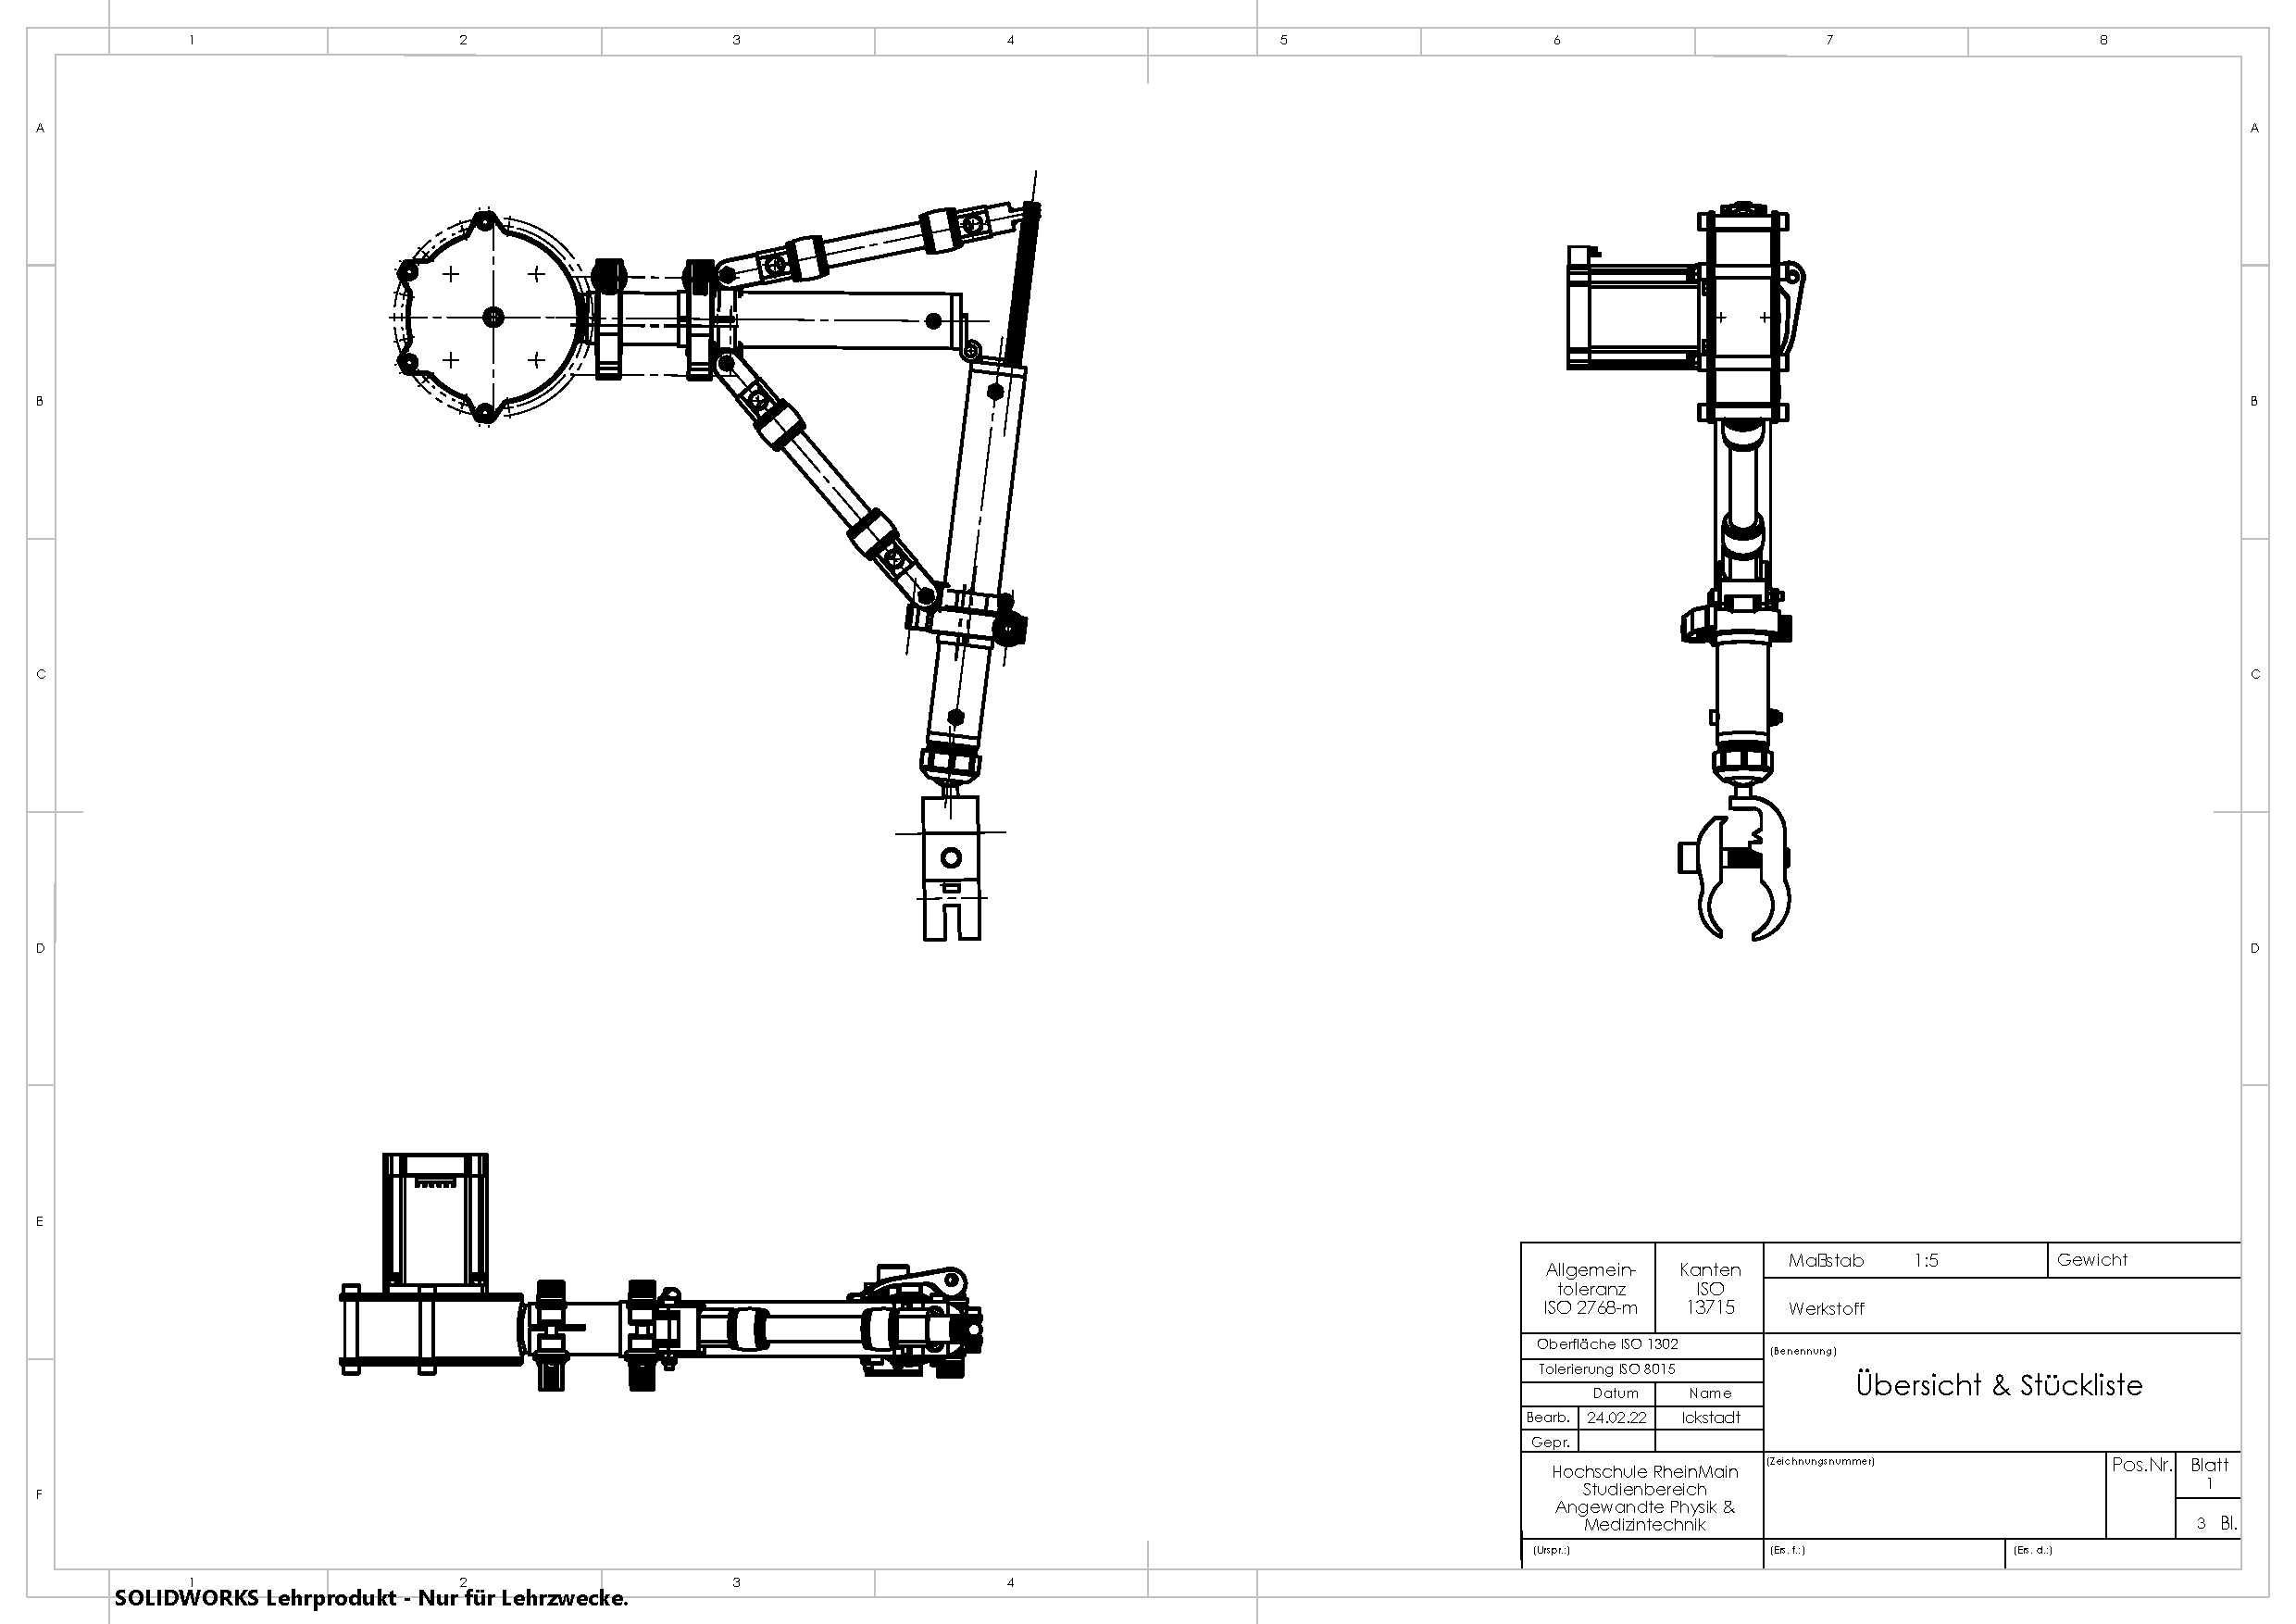
\includepdf[pages=1, angle=90, pagecommand={\thispagestyle{plain}}, addtolist={1, figure, Übersicht und Stückliste, drw:Uebersicht und Stueckliste}, addtotoc={1, section, 1, Bauteilzeichnungen, sec:bauteilzeichnungen}]{Abb/CAD/Drawings/Uebersicht-und-Stueckliste.pdf}
\includepdf[pages=2, angle=90, pagecommand={\thispagestyle{plain}}]{Abb/CAD/Drawings/Uebersicht-und-Stueckliste.pdf}
%
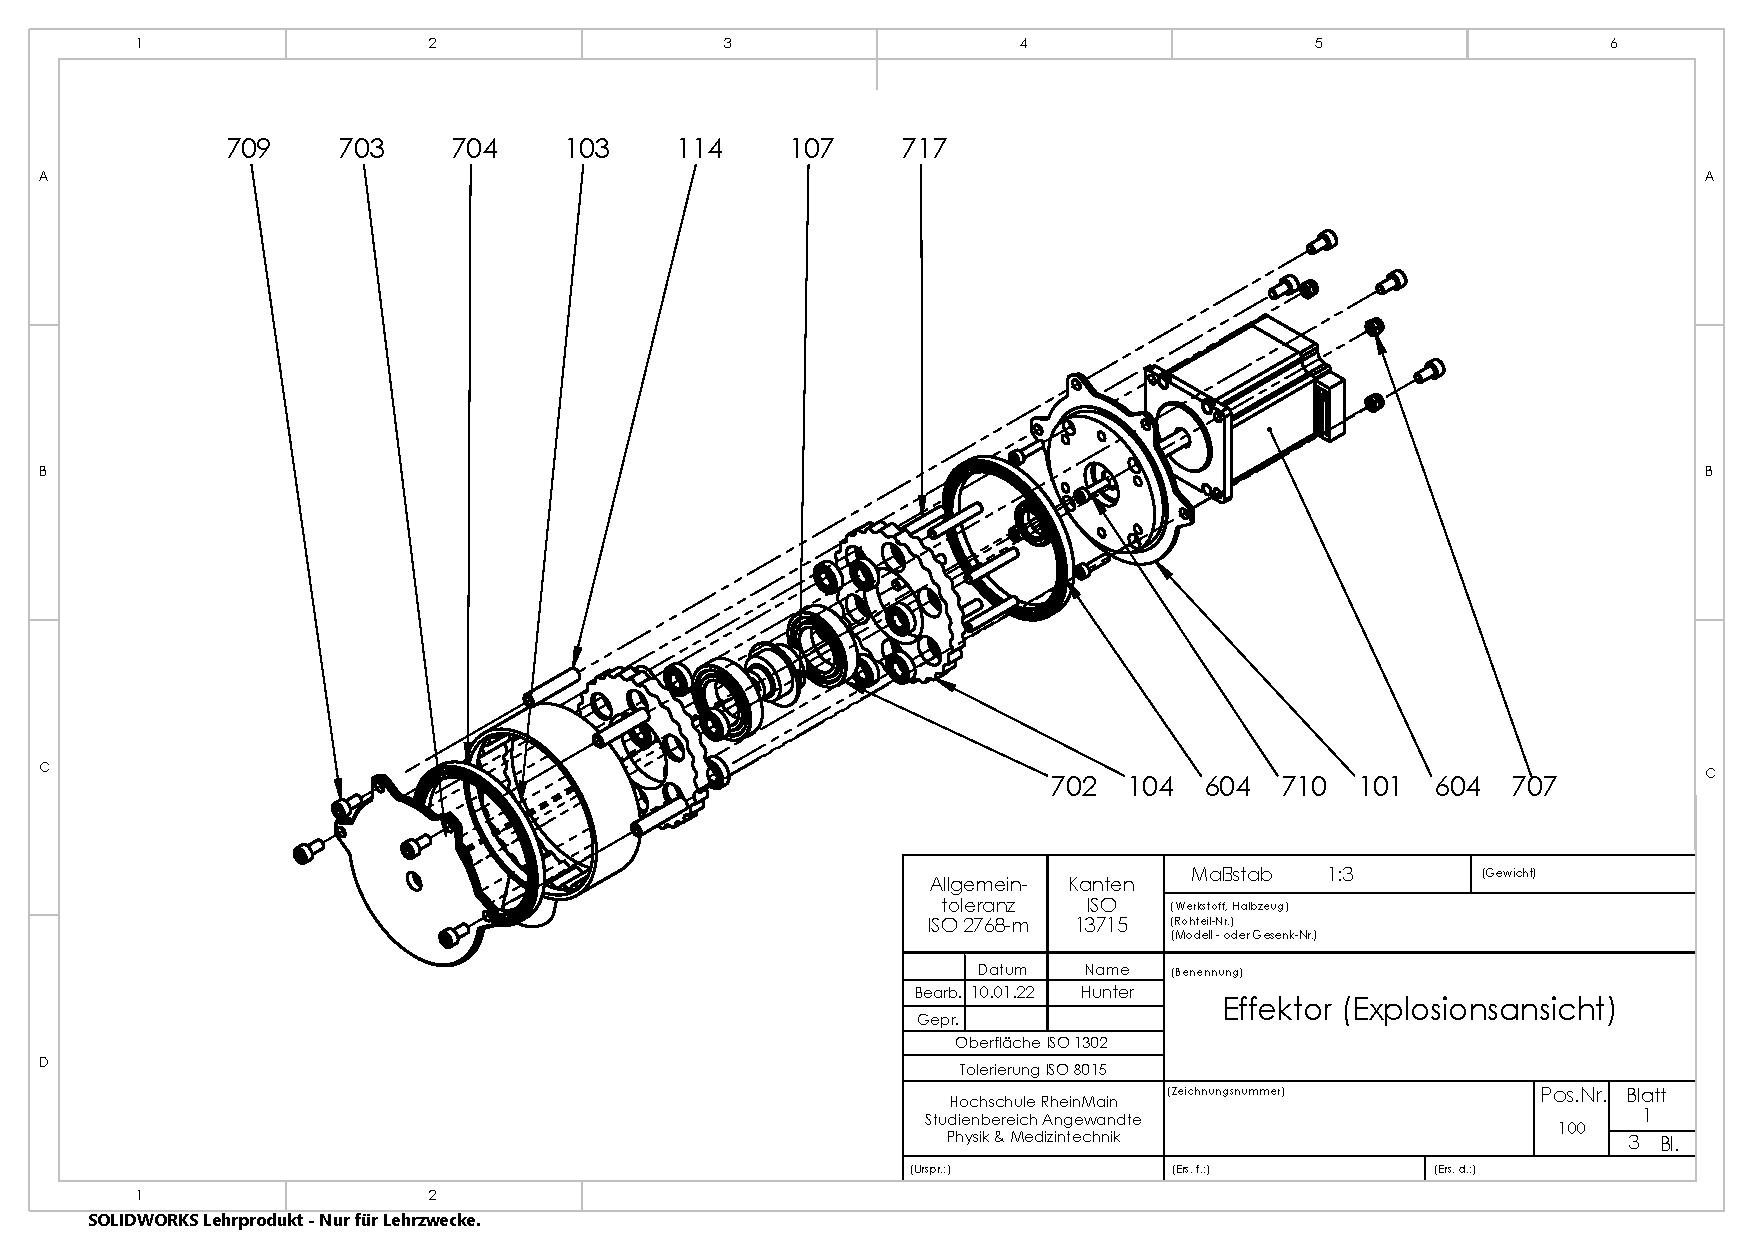
\includepdf[pages=1, angle=90, pagecommand={\thispagestyle{plain}}, addtolist={1, figure, Effektor, drw:Effektor}]{Abb/CAD/Drawings/Schulter/Effektor-assembly-drawing.pdf}
\includepdf[pages=2-3, angle=0, pagecommand={\thispagestyle{plain}}]{Abb/CAD/Drawings/Schulter/Effektor-assembly-drawing.pdf}
%
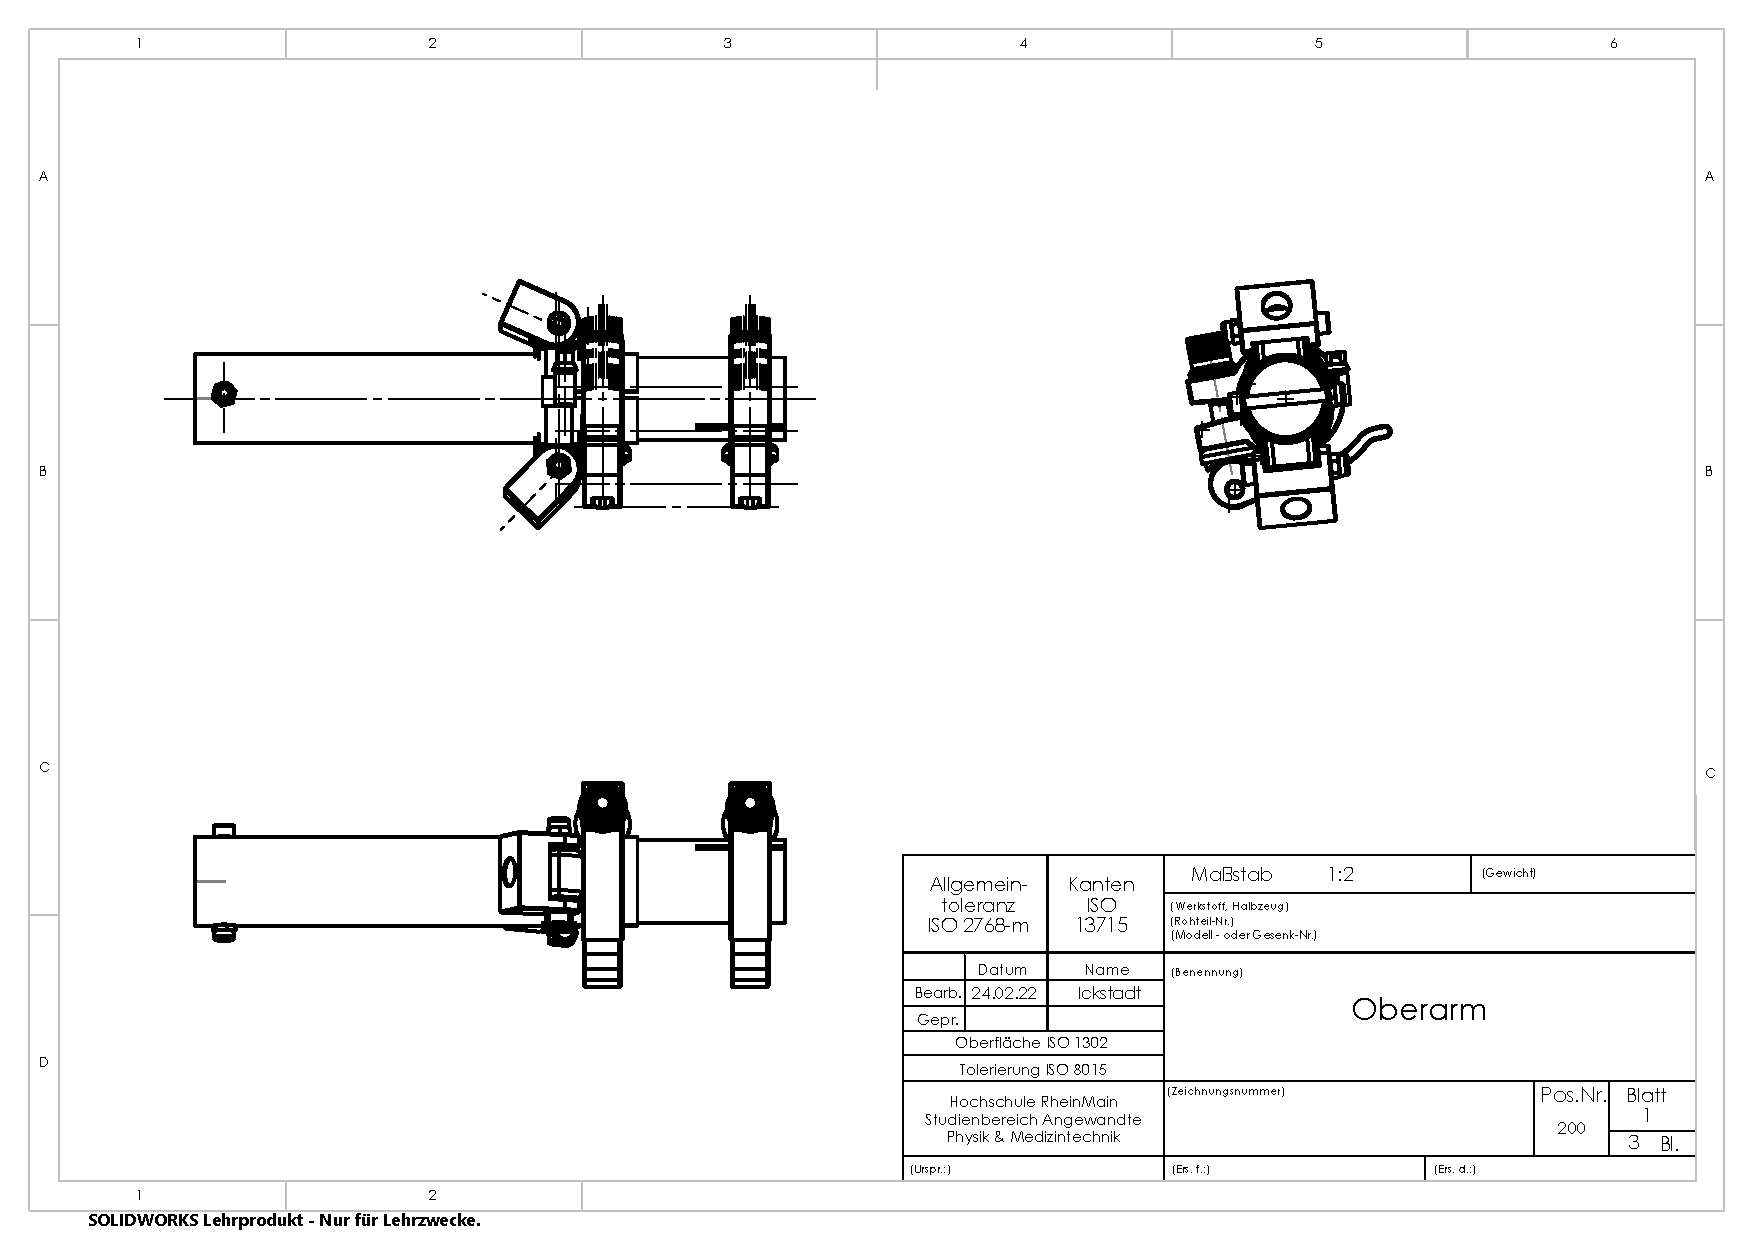
\includepdf[pages=1-2, angle=90, pagecommand={\thispagestyle{plain}}, addtolist={1, figure, Oberarm, drw:Oberarm}]{Abb/CAD/Drawings/Oberarm.pdf}
\includepdf[pages=3, angle=0, pagecommand={\thispagestyle{plain}}]{Abb/CAD/Drawings/Oberarm.pdf}
%
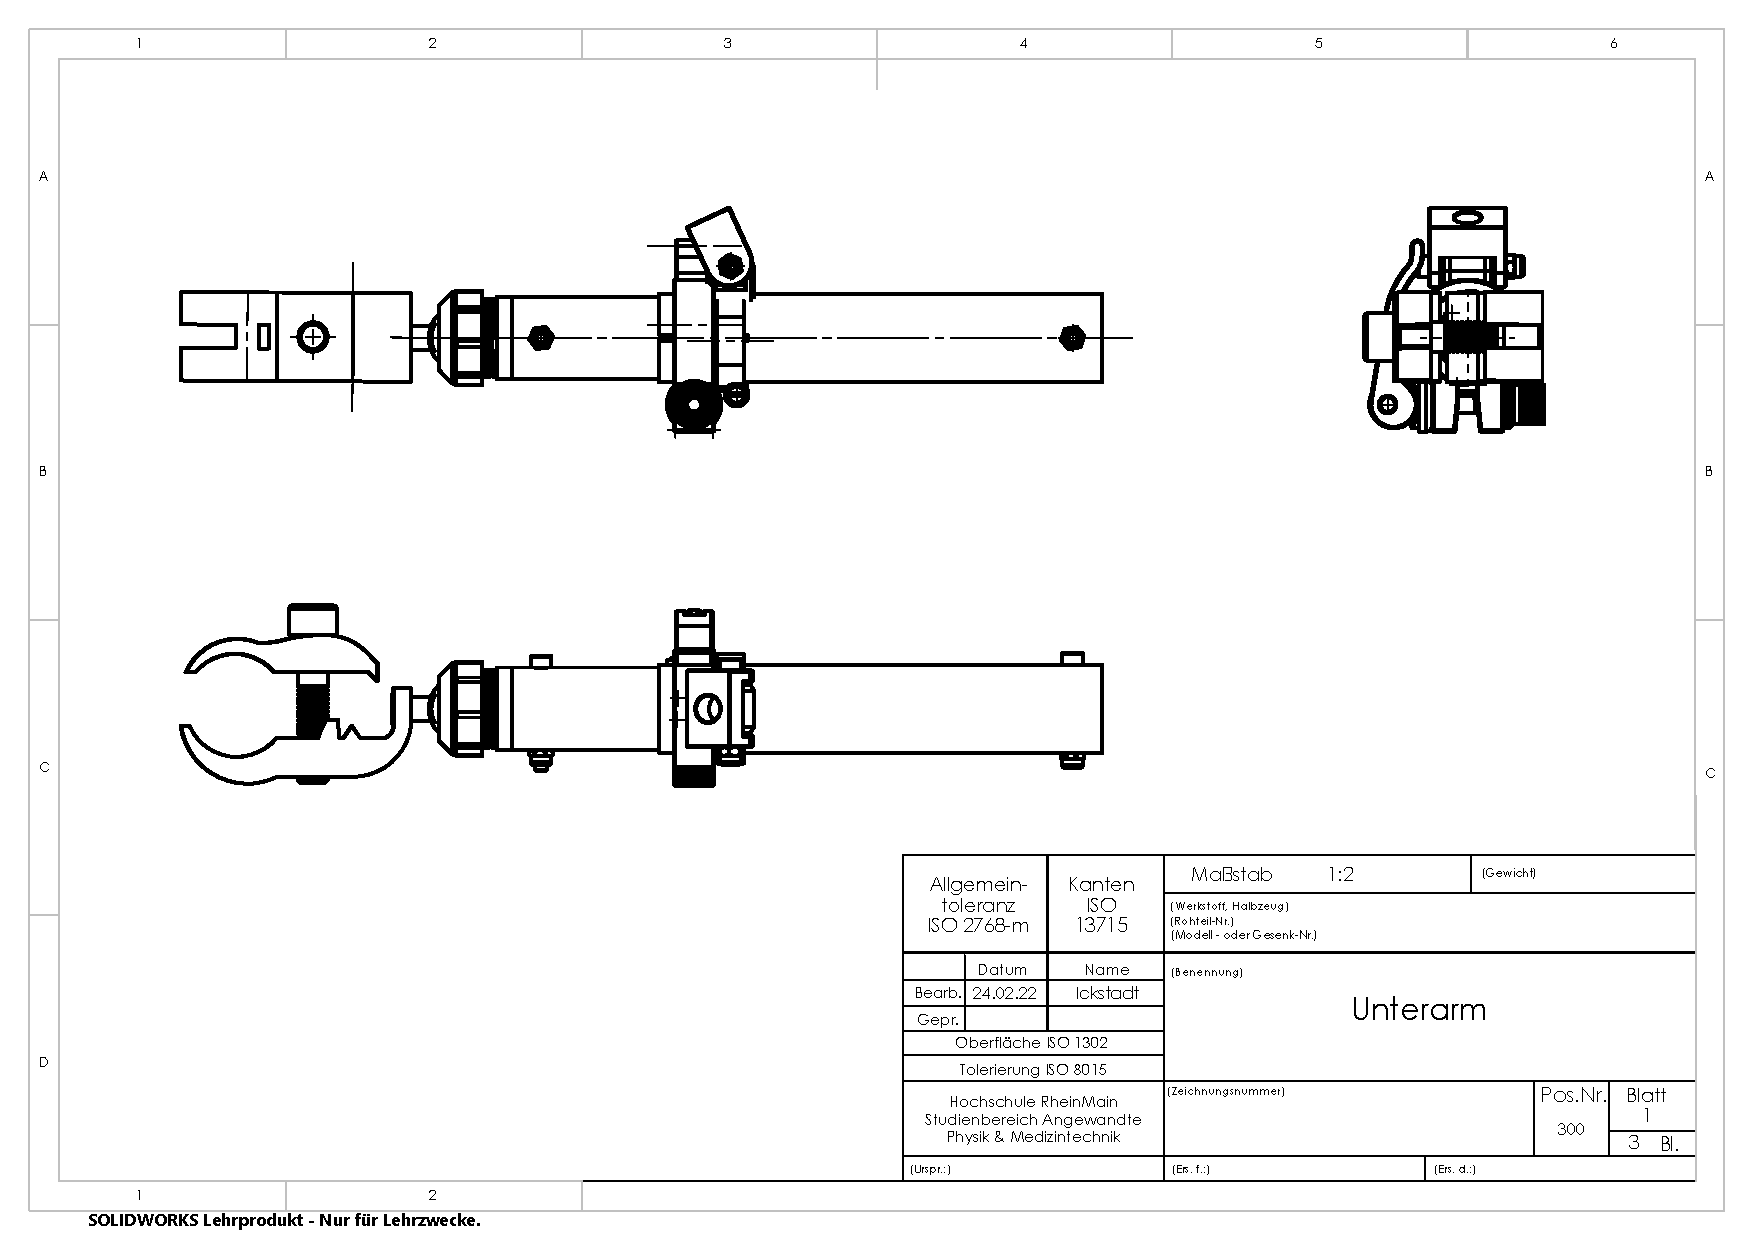
\includepdf[pages=1-2, angle=90, pagecommand={\thispagestyle{plain}}, addtolist={1, figure, Unterarm, drw:Unterarm}]{Abb/CAD/Drawings/Unterarm.pdf}
\includepdf[pages=3, angle=0, pagecommand={\thispagestyle{plain}}]{Abb/CAD/Drawings/Unterarm.pdf}
%
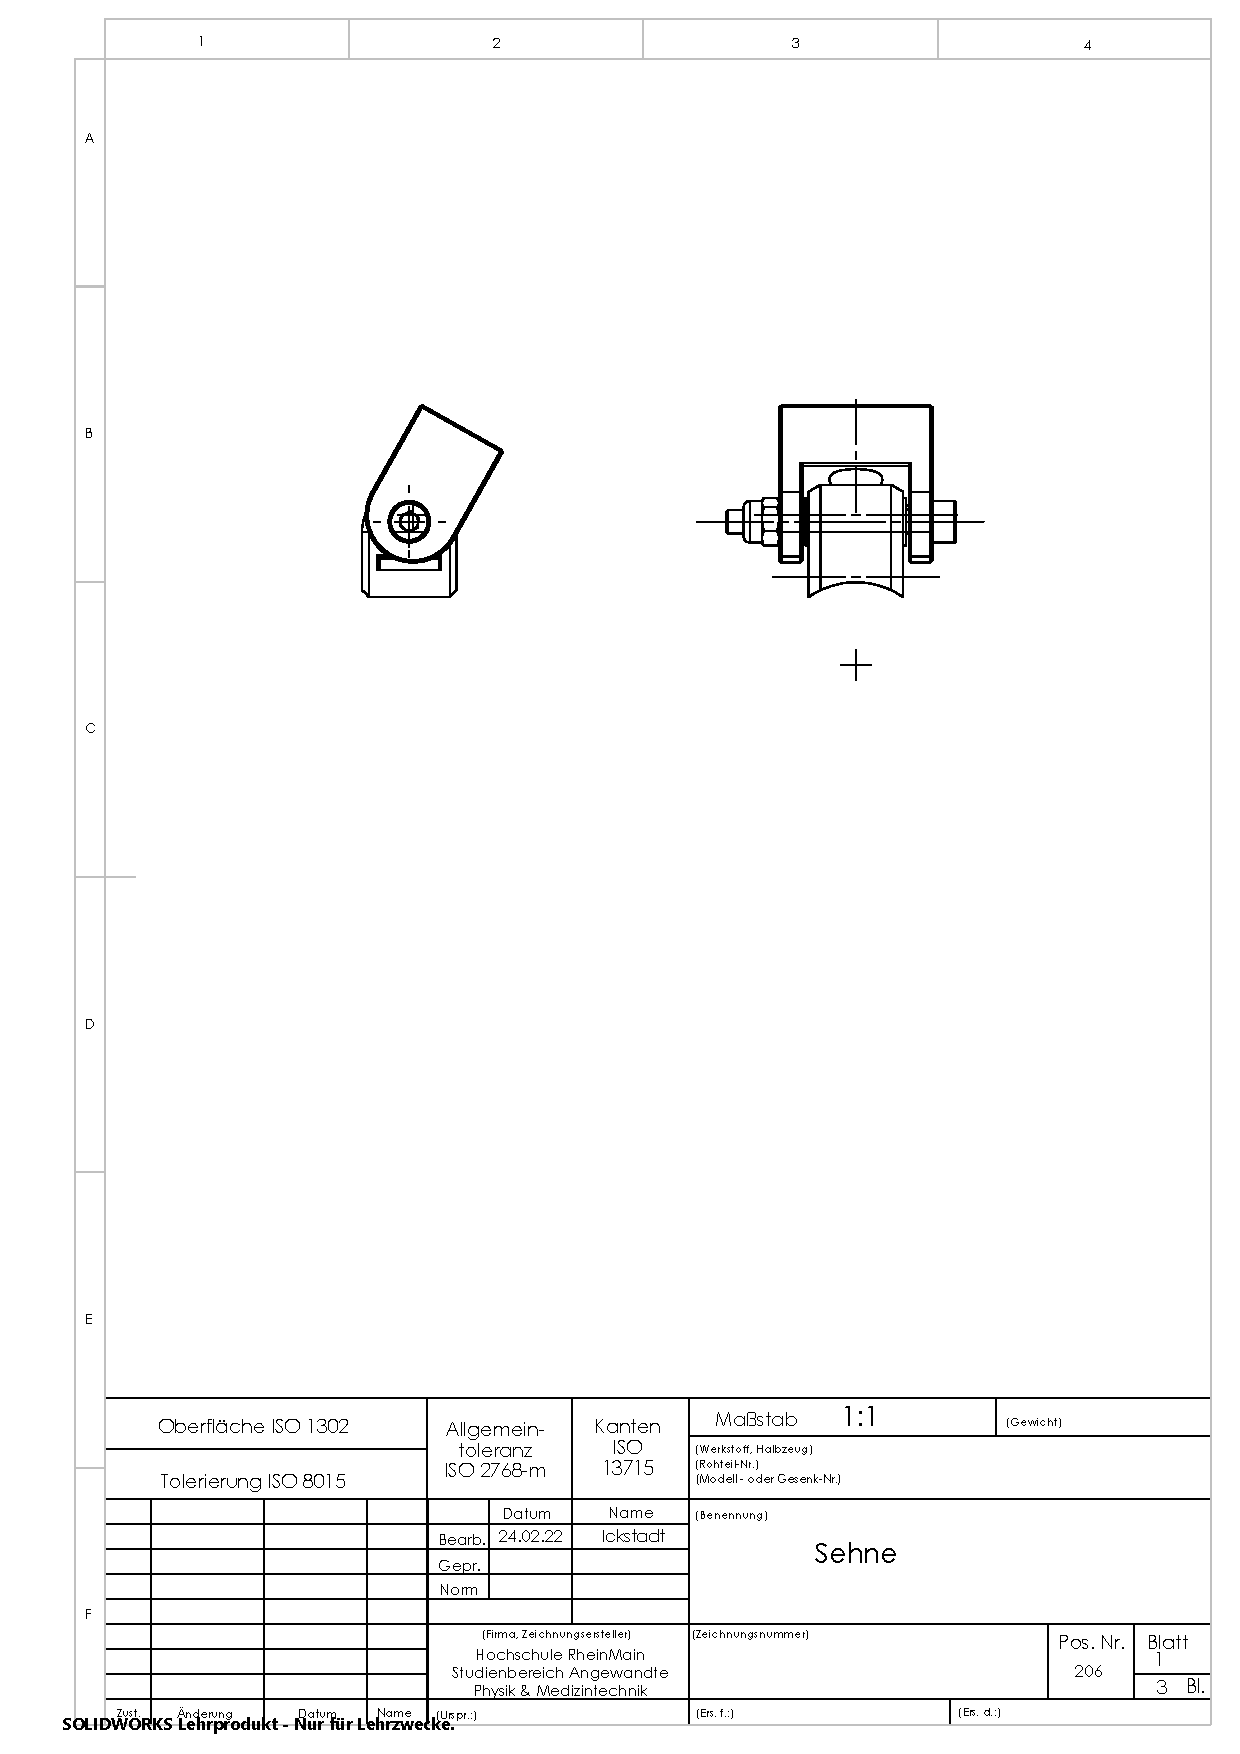
\includepdf[pages=-, angle=0, pagecommand={\thispagestyle{plain}}, addtolist={1, figure, Sehne, drw:Sehne}]{Abb/CAD/Drawings/Sehne.pdf}
%
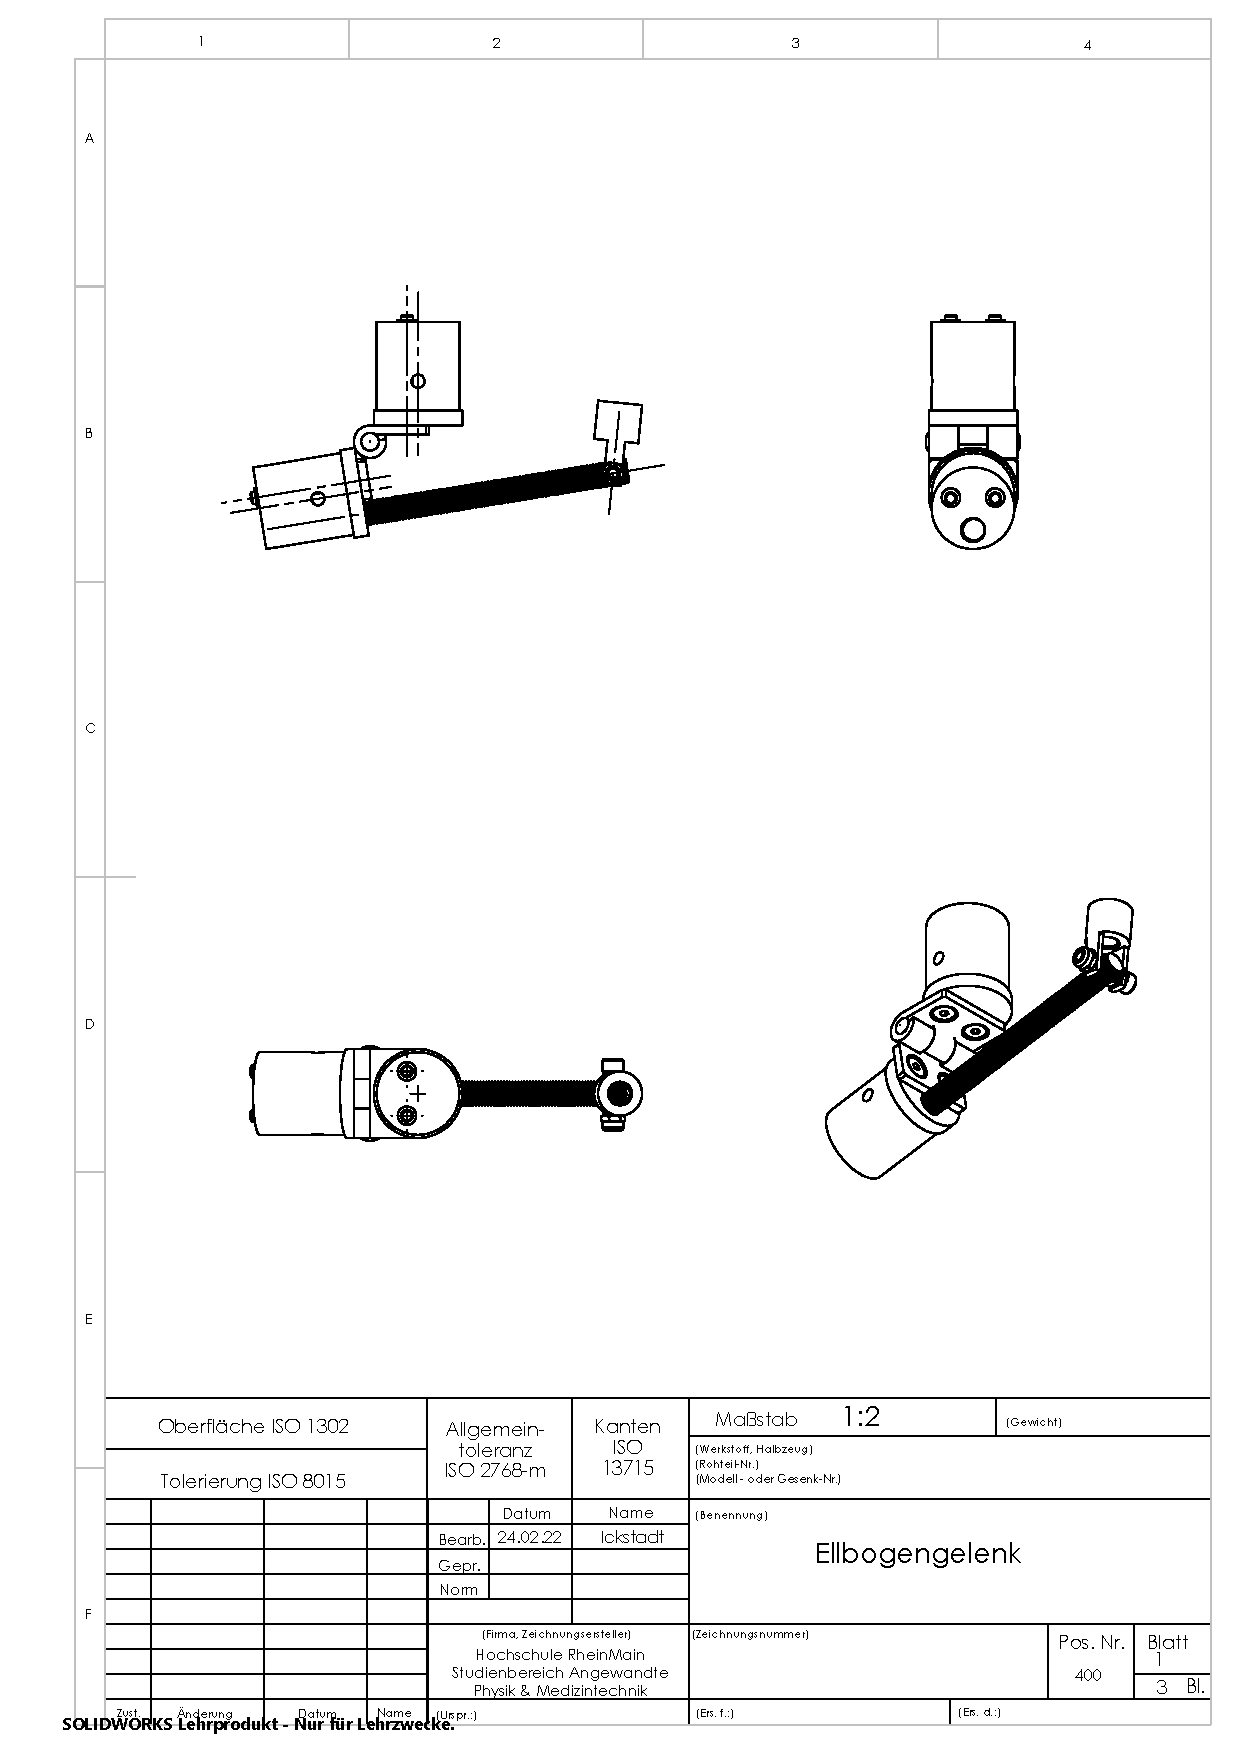
\includepdf[pages=-, angle=0, pagecommand={\thispagestyle{plain}}, addtolist={1, figure, Ellbogengelenk, drw:Ellbogengelenk}]{Abb/CAD/Drawings/Ellbogengelenk.pdf}
%
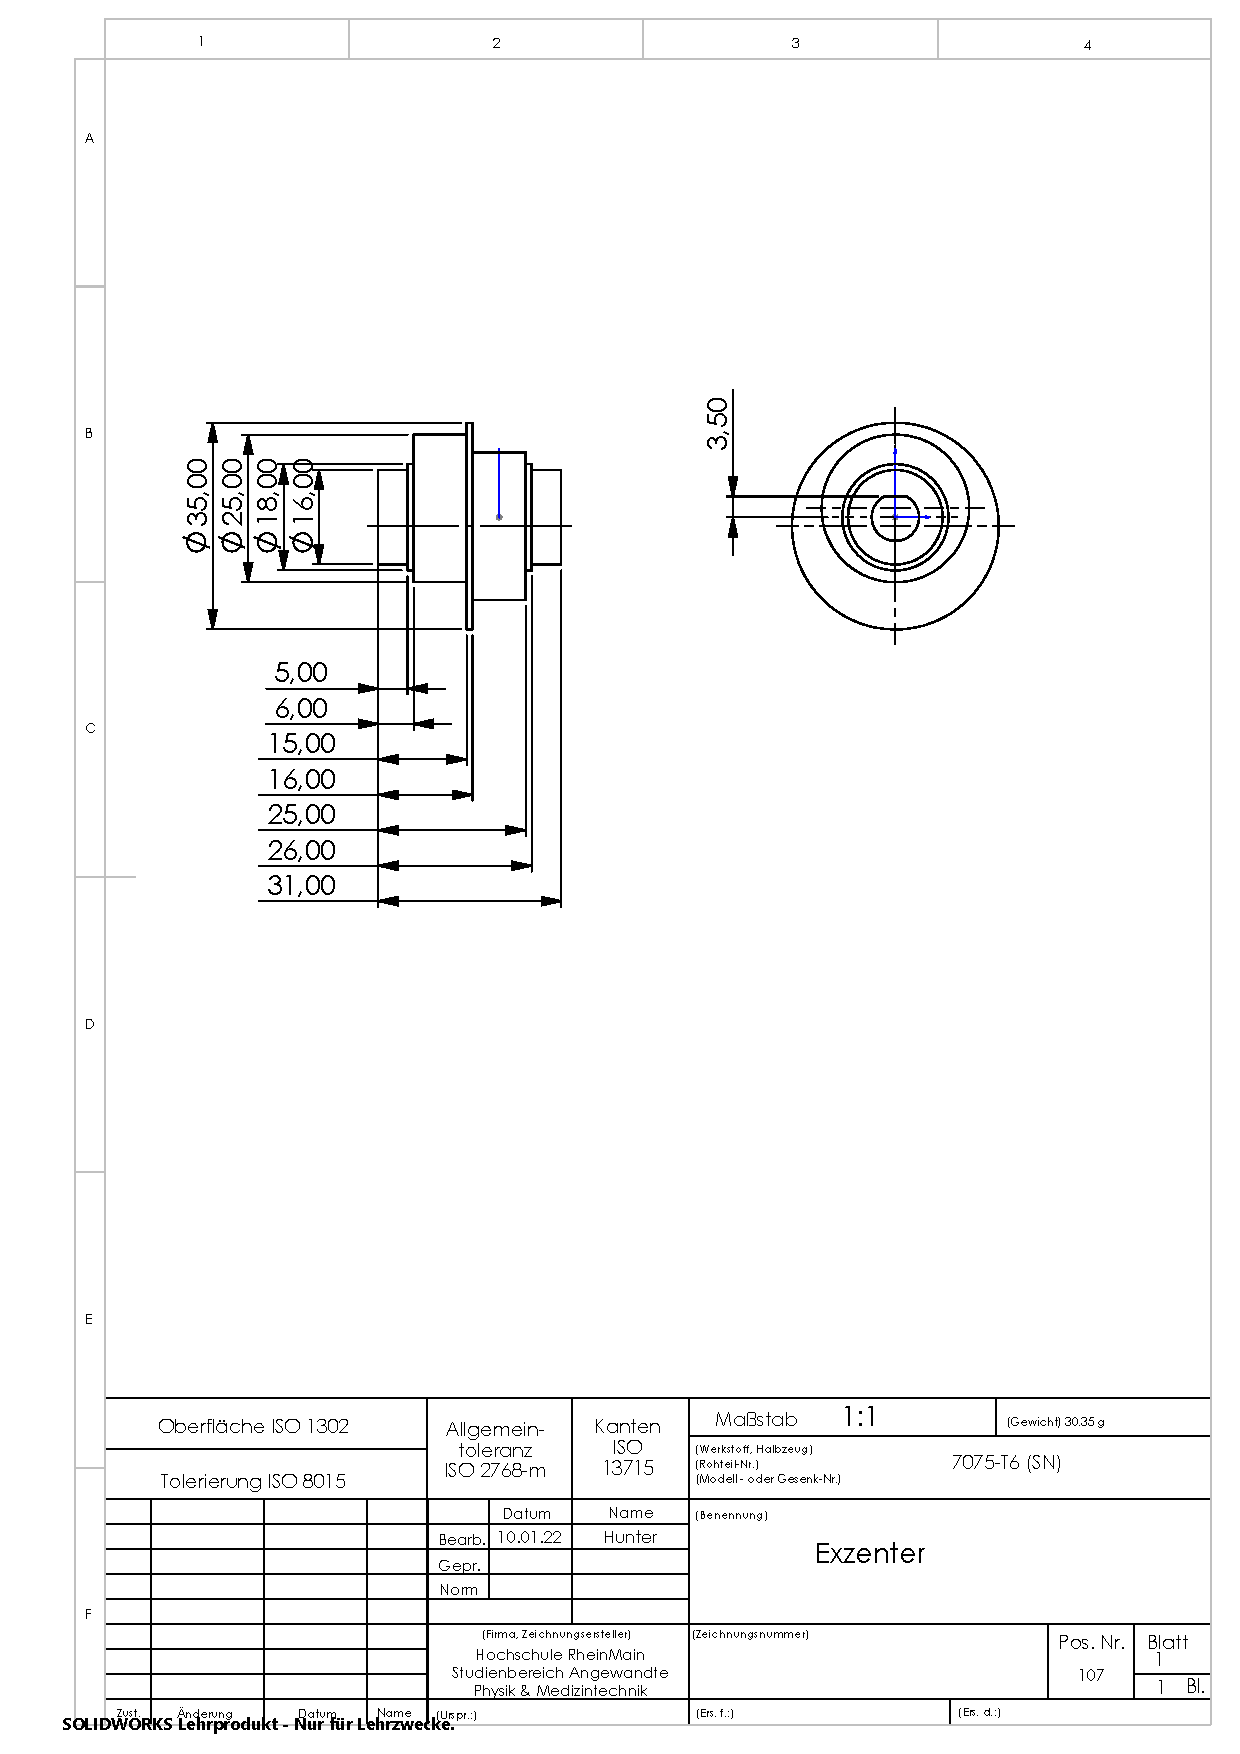
\includepdf[pages=-, angle=0, pagecommand={\thispagestyle{plain}}, addtolist={1, figure, Exzenter, drw:Exzenter}, addtotoc={1, section, 1, Einzelteilzeichnungen Schultergelenk, {sec:einzelteilzeichnungen schultergelenk}}]{Abb/CAD/Drawings/Schulter/Exzenter.pdf}
%
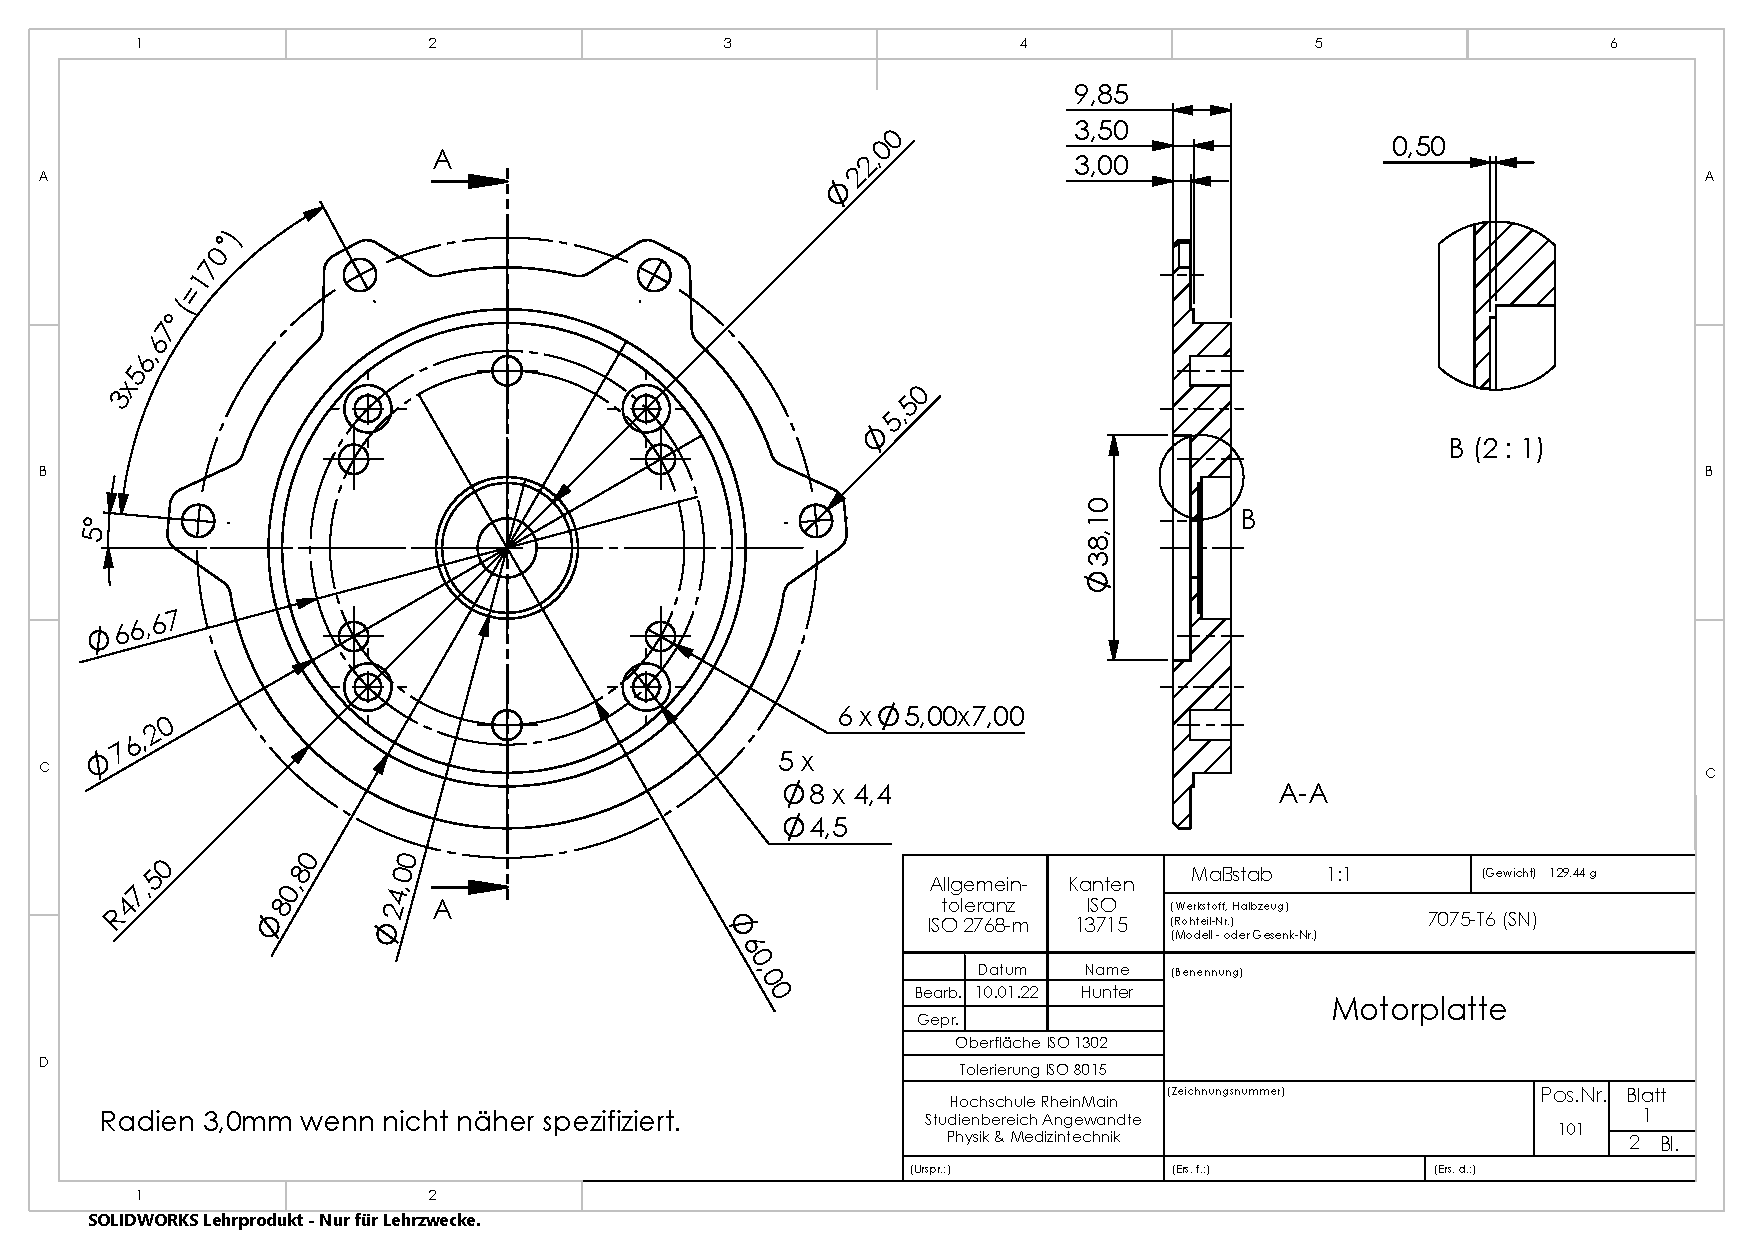
\includepdf[pages=-, angle=90, pagecommand={\thispagestyle{plain}}, addtolist={1, figure, Motor- und Fixierplatte, drw:Motor und Fixierplatte}]{Abb/CAD/Drawings/Schulter/Motorplatte-Fixierplatte.pdf}
%
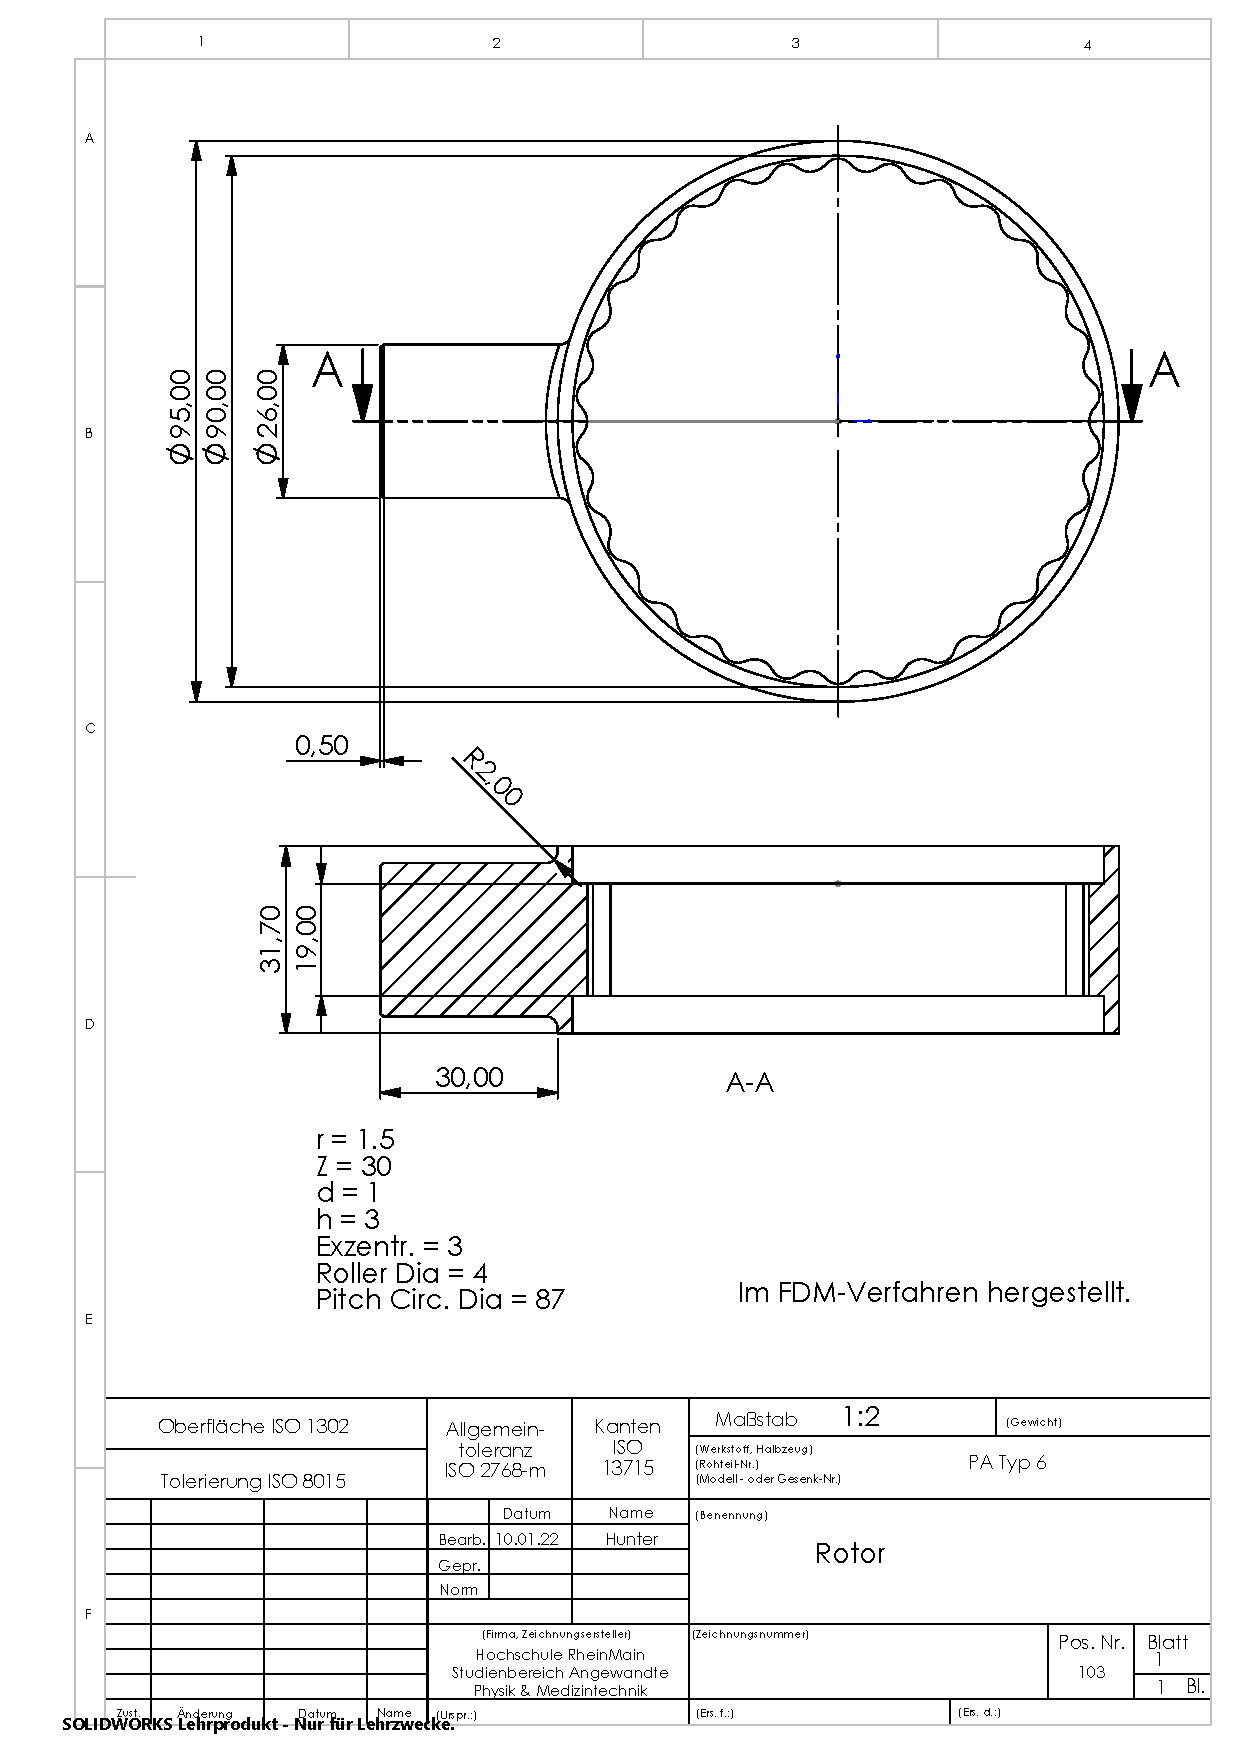
\includepdf[pages=-, angle=0, pagecommand={\thispagestyle{plain}}, addtolist={1, figure, Rotor, drw:Rotor}]{Abb/CAD/Drawings/Schulter/Rotor.pdf}
%
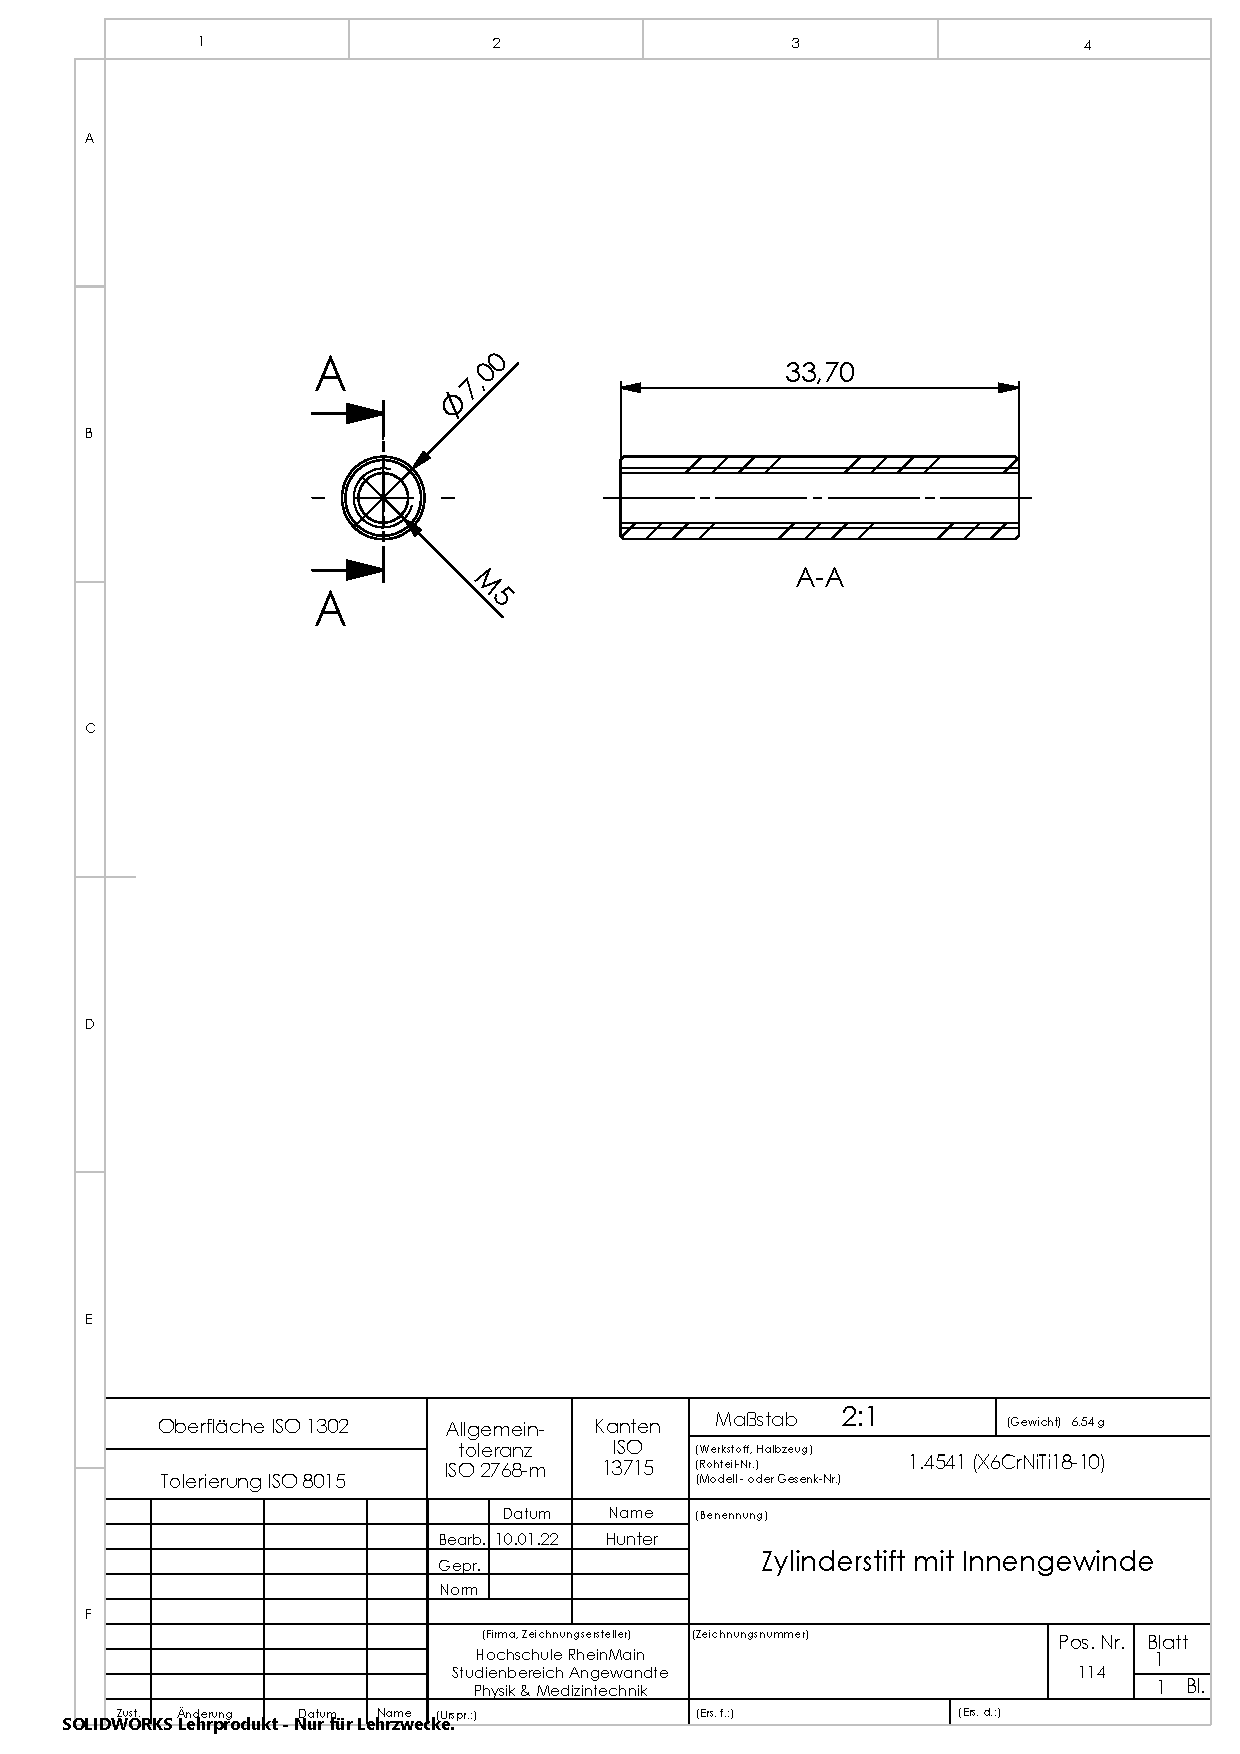
\includepdf[pages=-, angle=0, pagecommand={\thispagestyle{plain}}, addtolist={1, figure, Zylinderstift, drw:Zylinderstift}]{Abb/CAD/Drawings/Schulter/Zylinderstift-mit-Innengewinde.pdf}
%
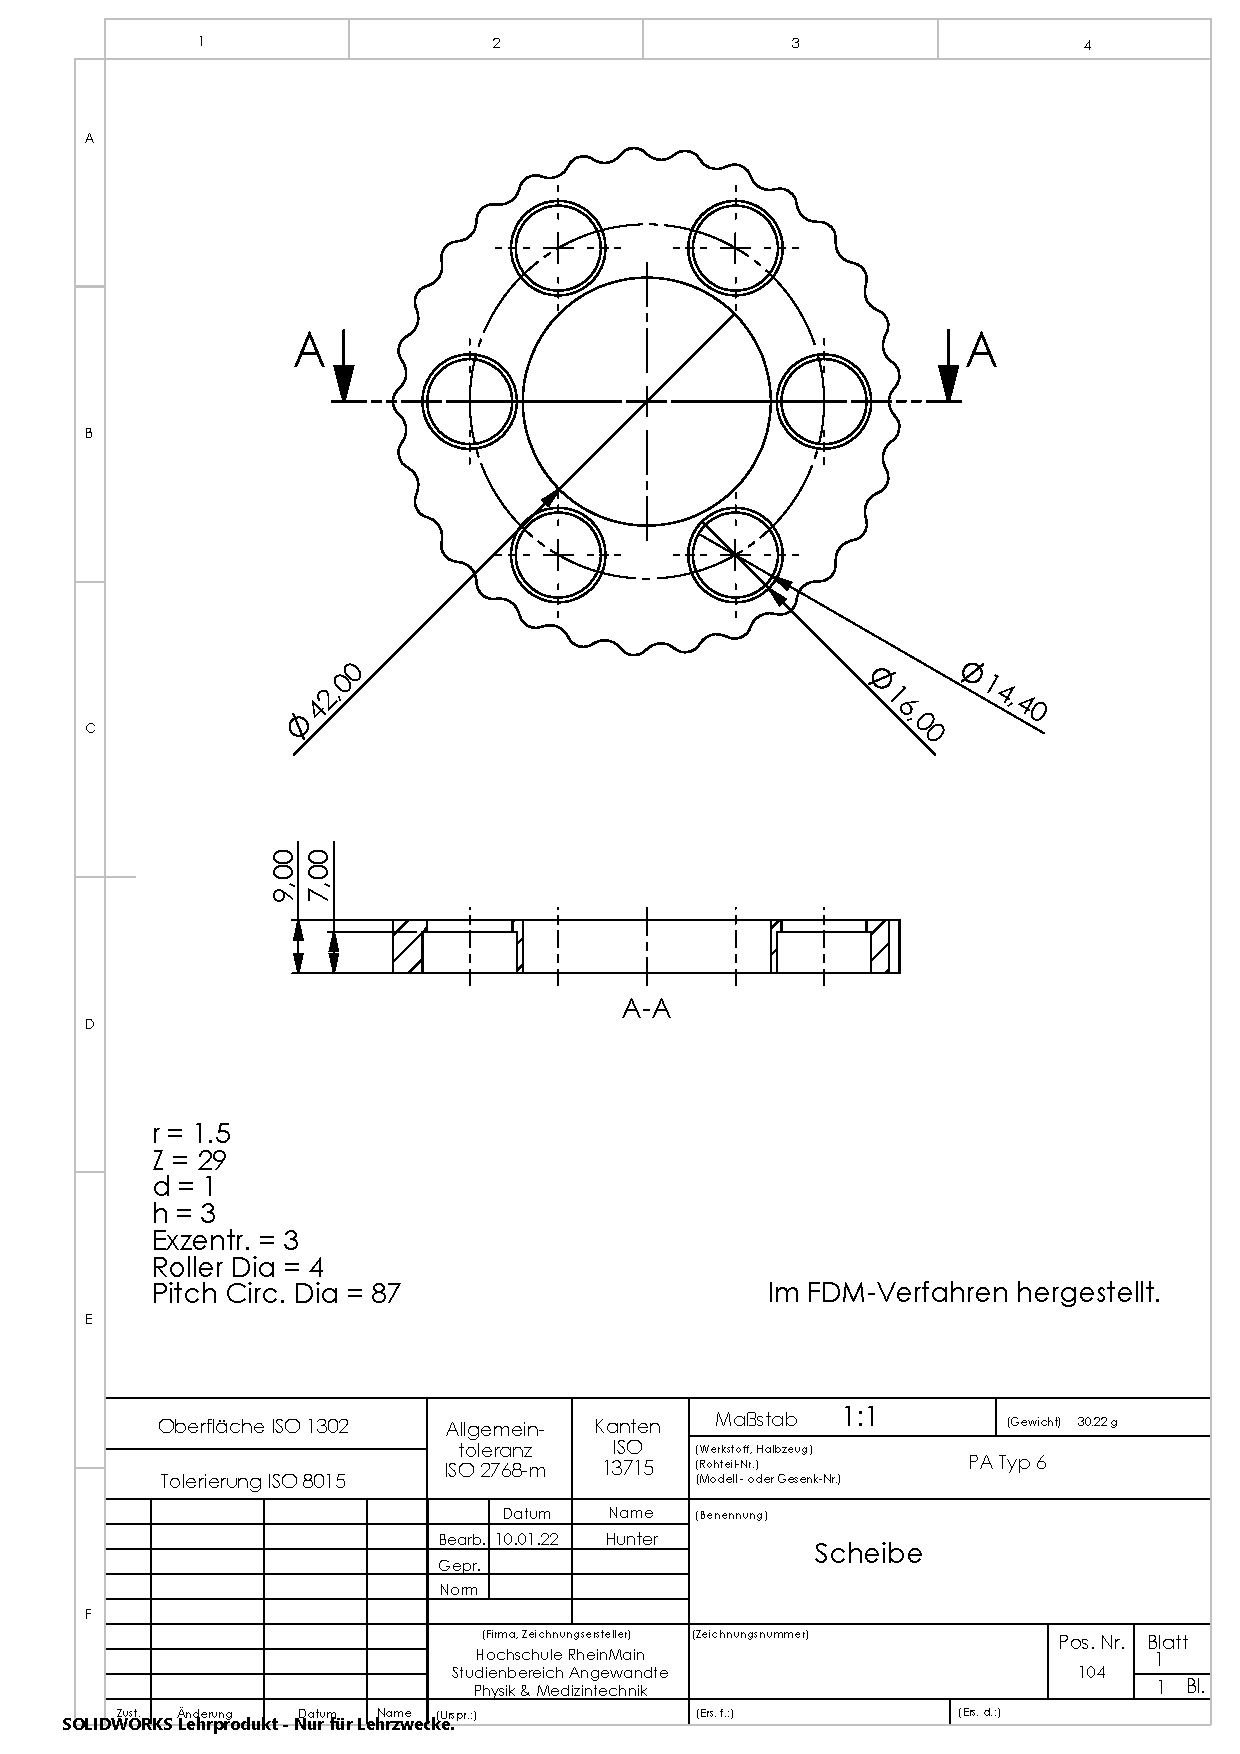
\includepdf[pages=-, angle=0, pagecommand={\thispagestyle{plain}}, addtolist={1, figure, Zahnscheibe, drw:Scheibe}]{Abb/CAD/Drawings/Schulter/Scheibe.pdf}
%
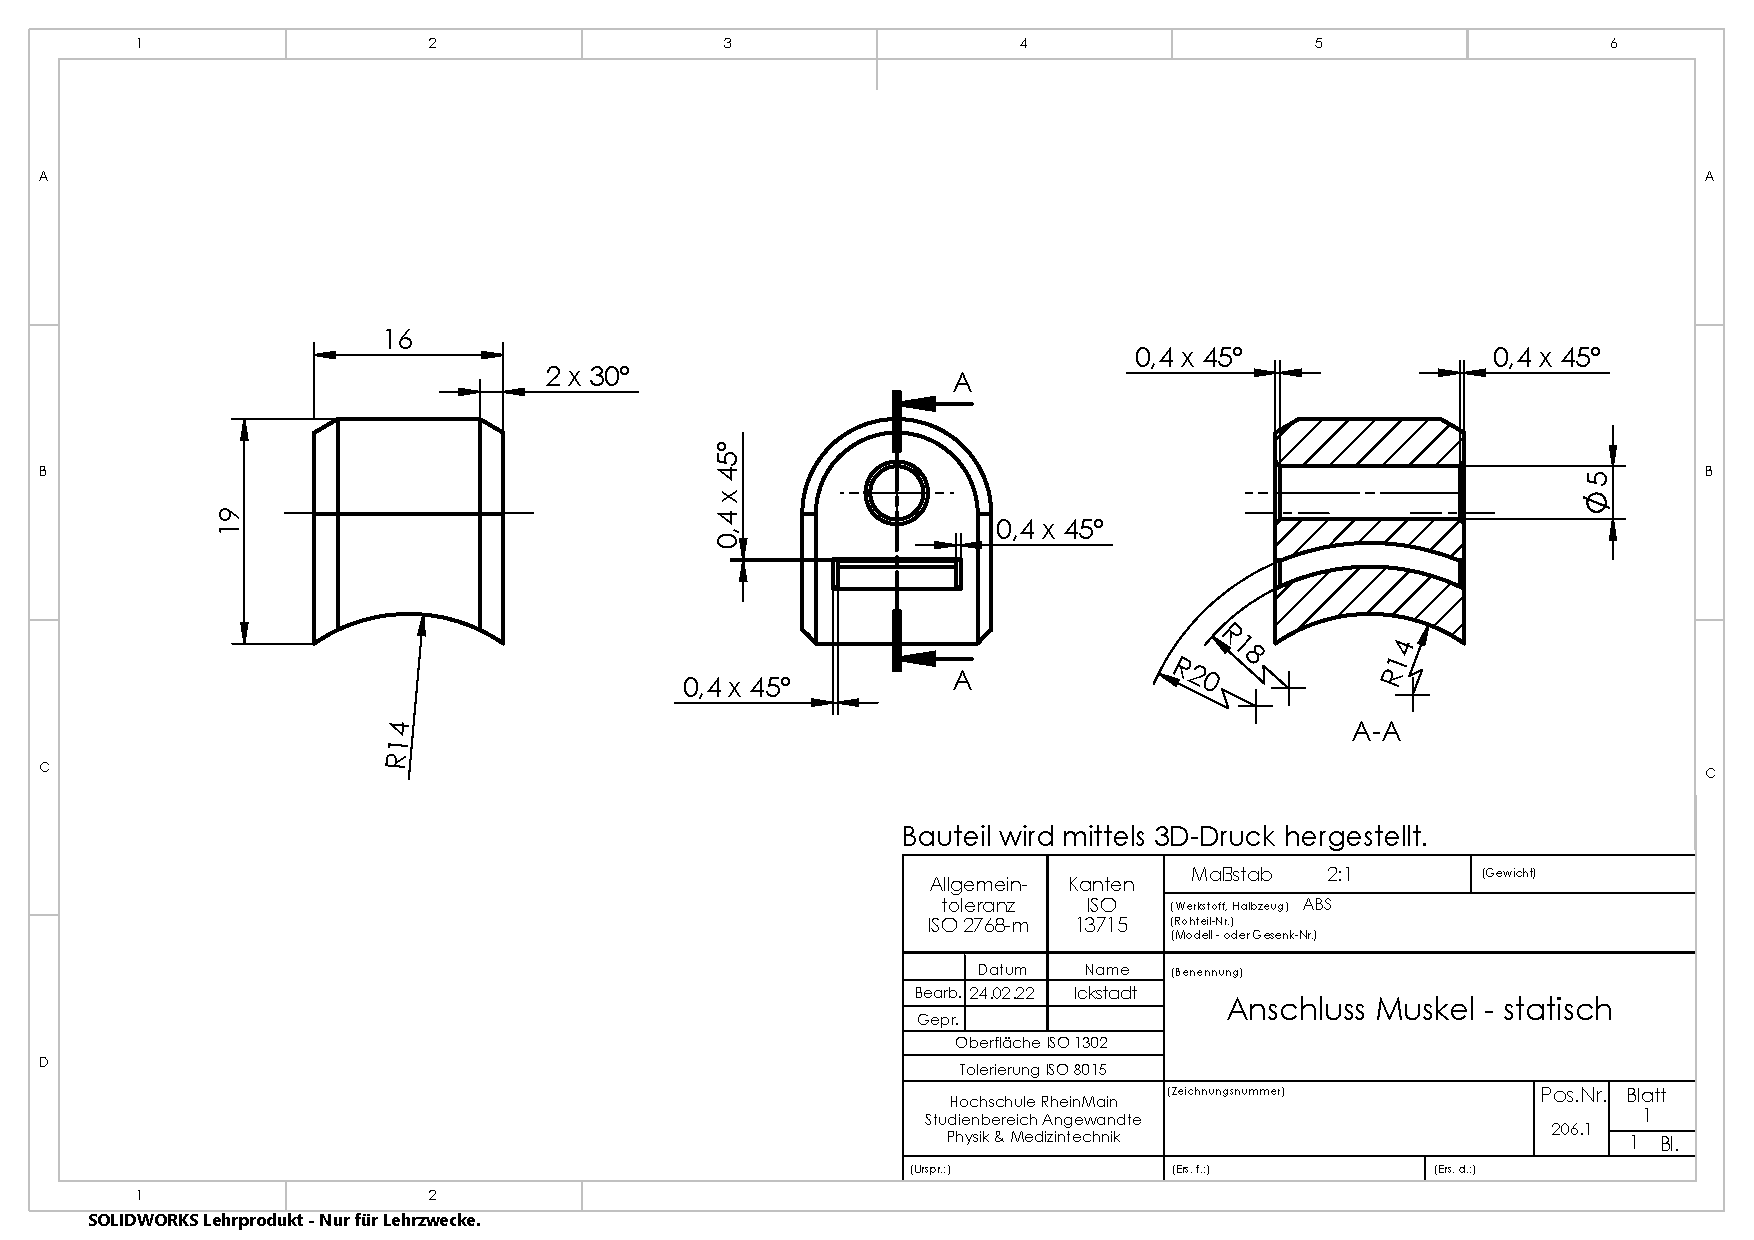
\includepdf[pages=-, angle=90, pagecommand={\thispagestyle{plain}}, addtolist={1, figure, Muskelanschluss, drw:Muskelanschluss}, addtotoc={1, section, 1, Einzelteilzeichnungen Arme, {sec:einzelteilzeichnungen arme}}]{Abb/CAD/Drawings/Anschluss-Muskel-statisch.pdf}
%
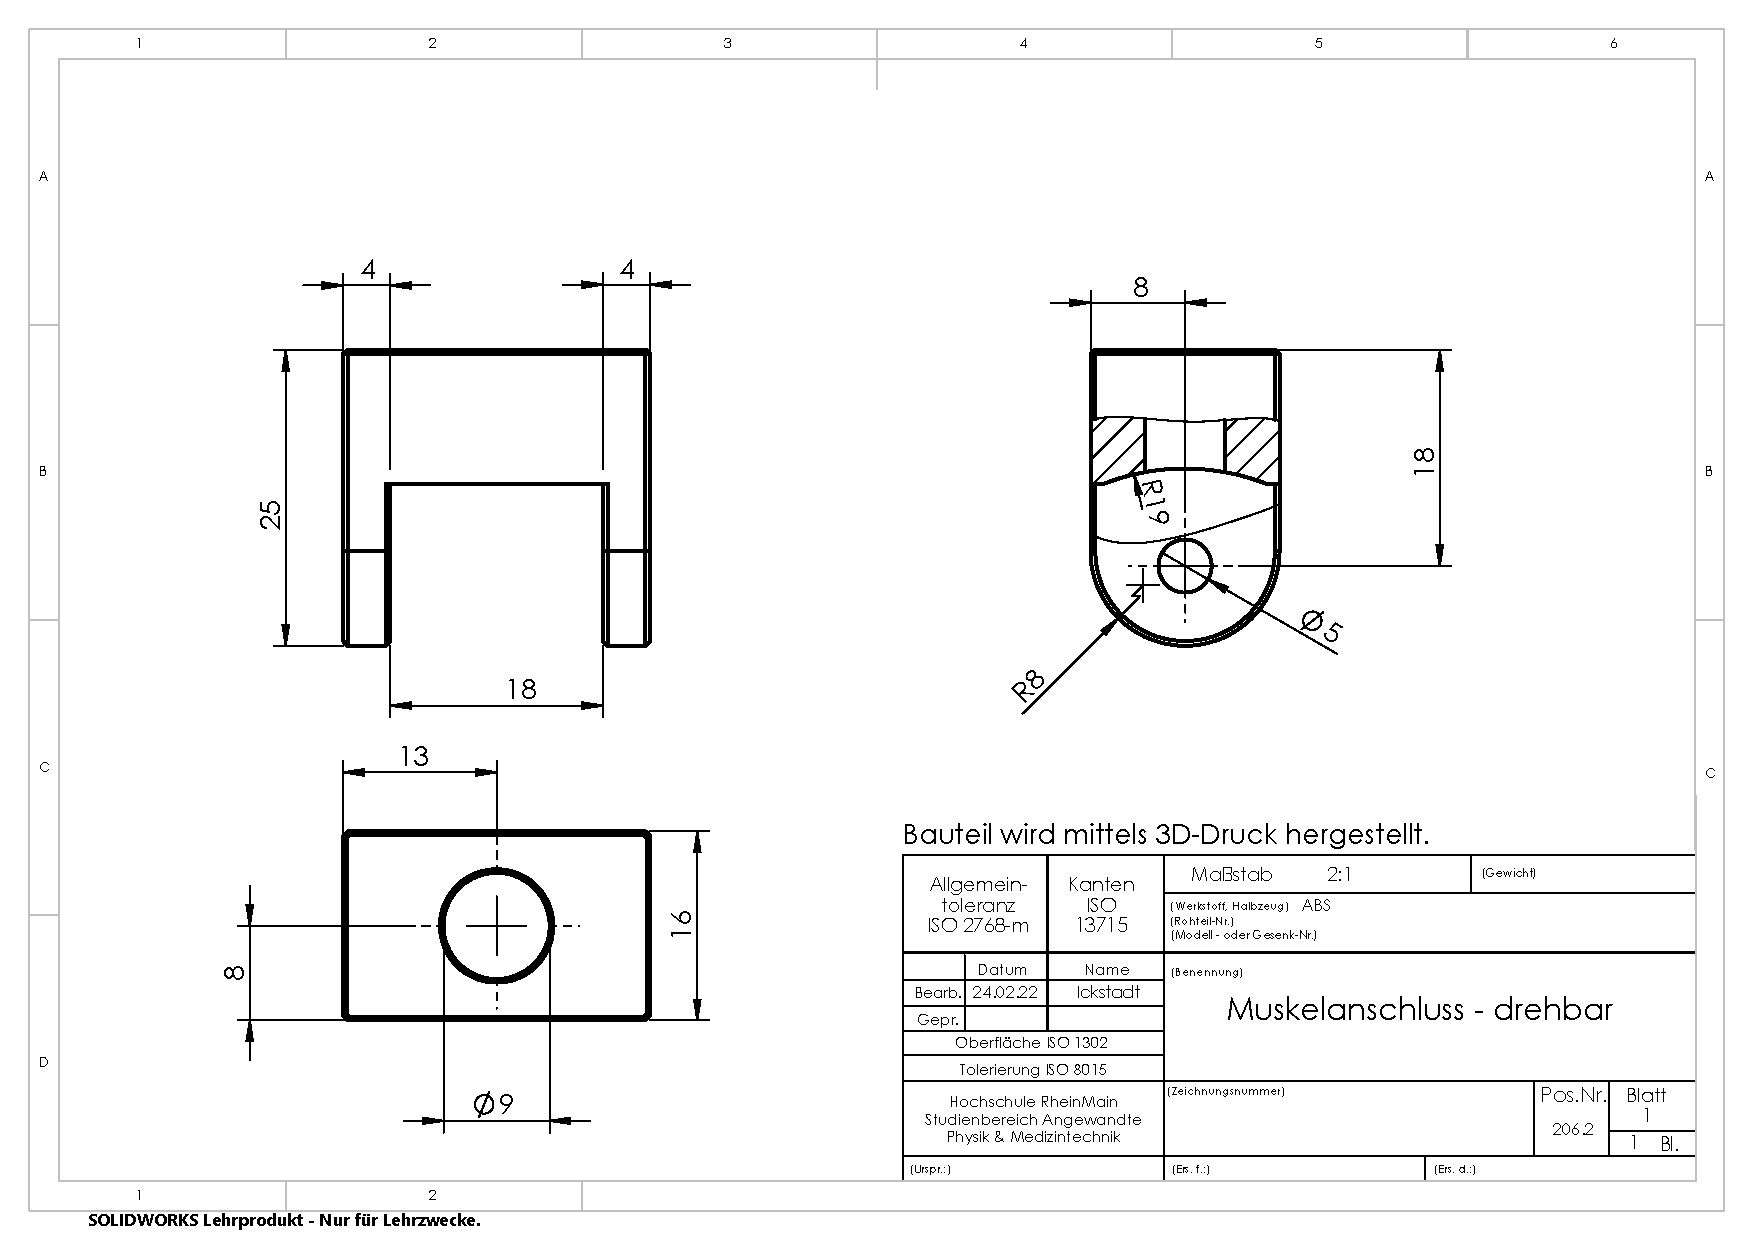
\includepdf[pages=-, angle=90, pagecommand={\thispagestyle{plain}}, addtolist={1, figure, Muskelanschluss drehbar, drw:Muskelanschluss-drehbar}]{Abb/CAD/Drawings/Muskelanschluss-drehbar.pdf}
%
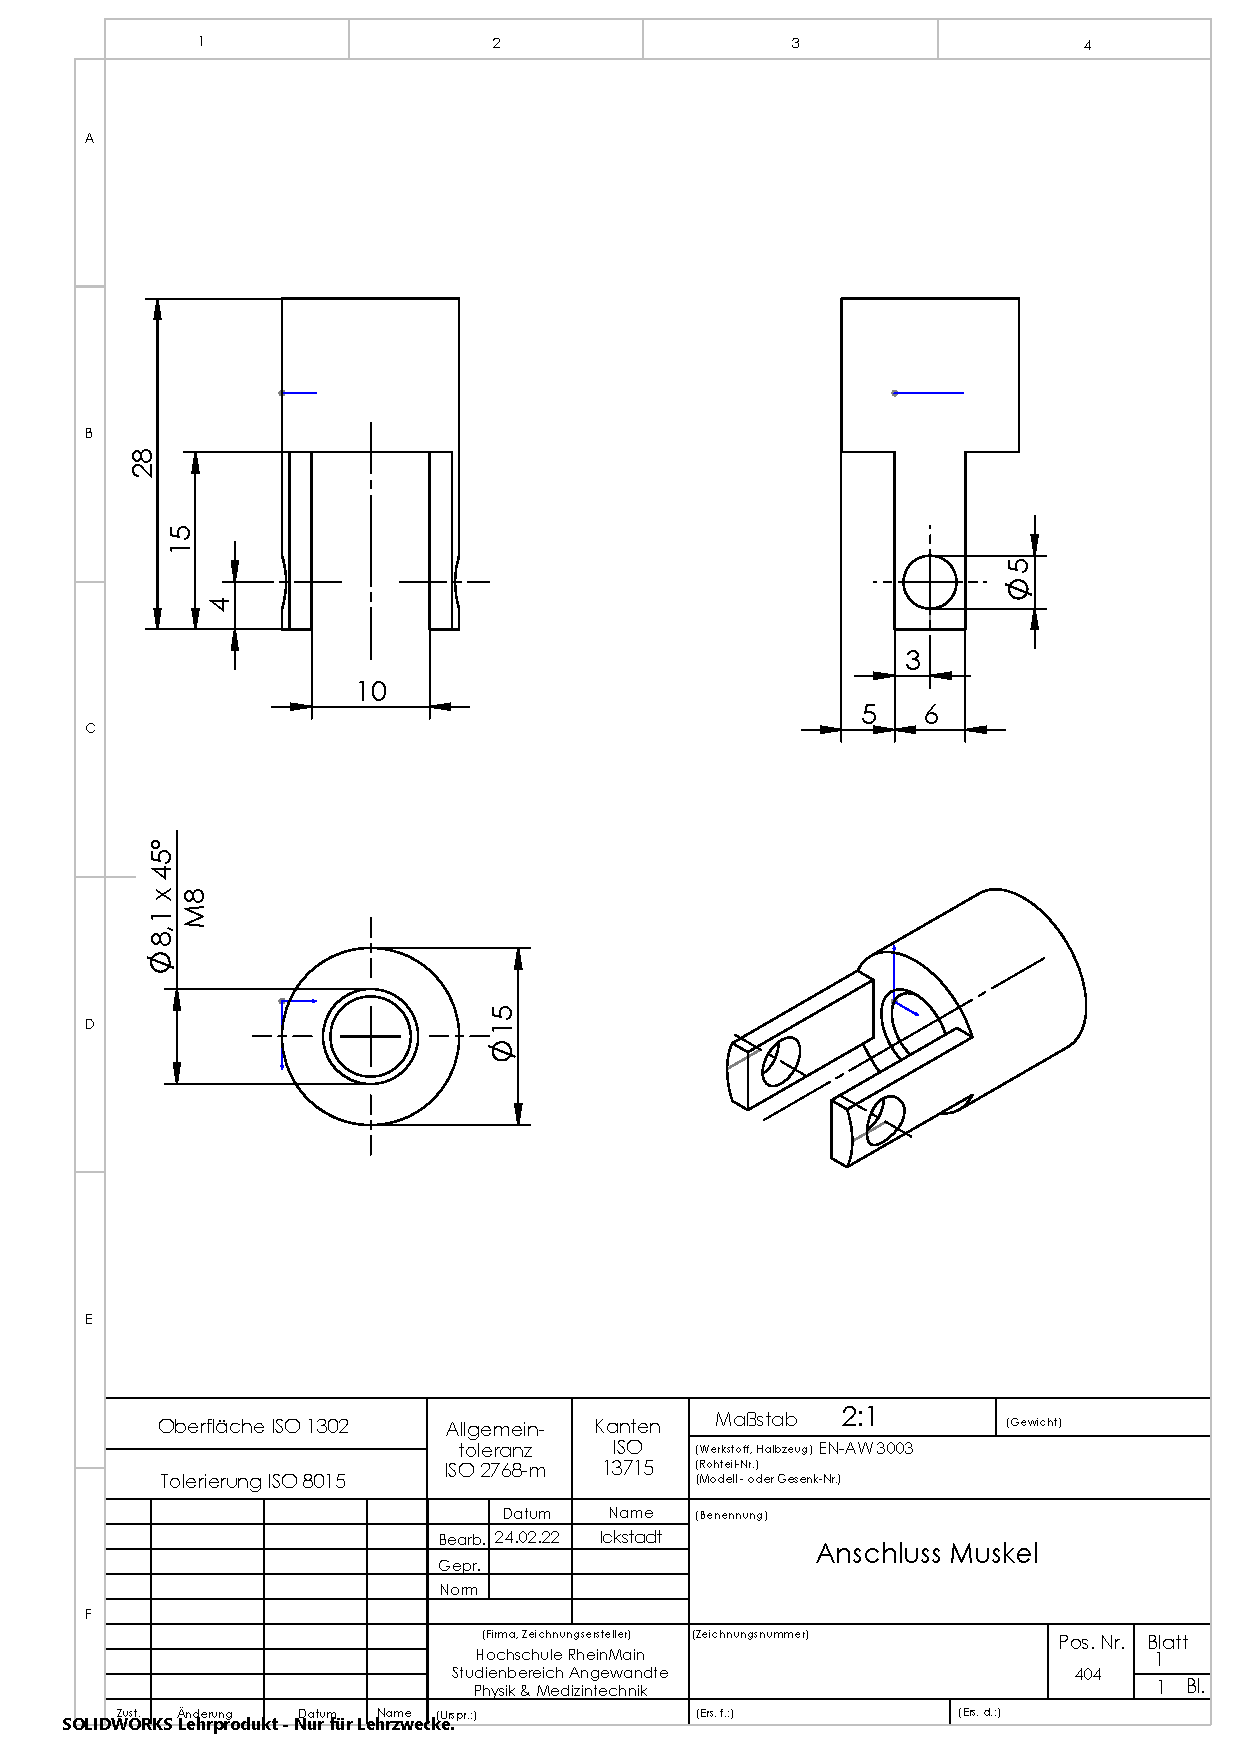
\includepdf[pages=-, angle=0, pagecommand={\thispagestyle{plain}}, addtolist={1, figure, Anschluss-Muskel, drw:Anschluss-Muskel}]{Abb/CAD/Drawings/Anschluss-Muskel.pdf}
%
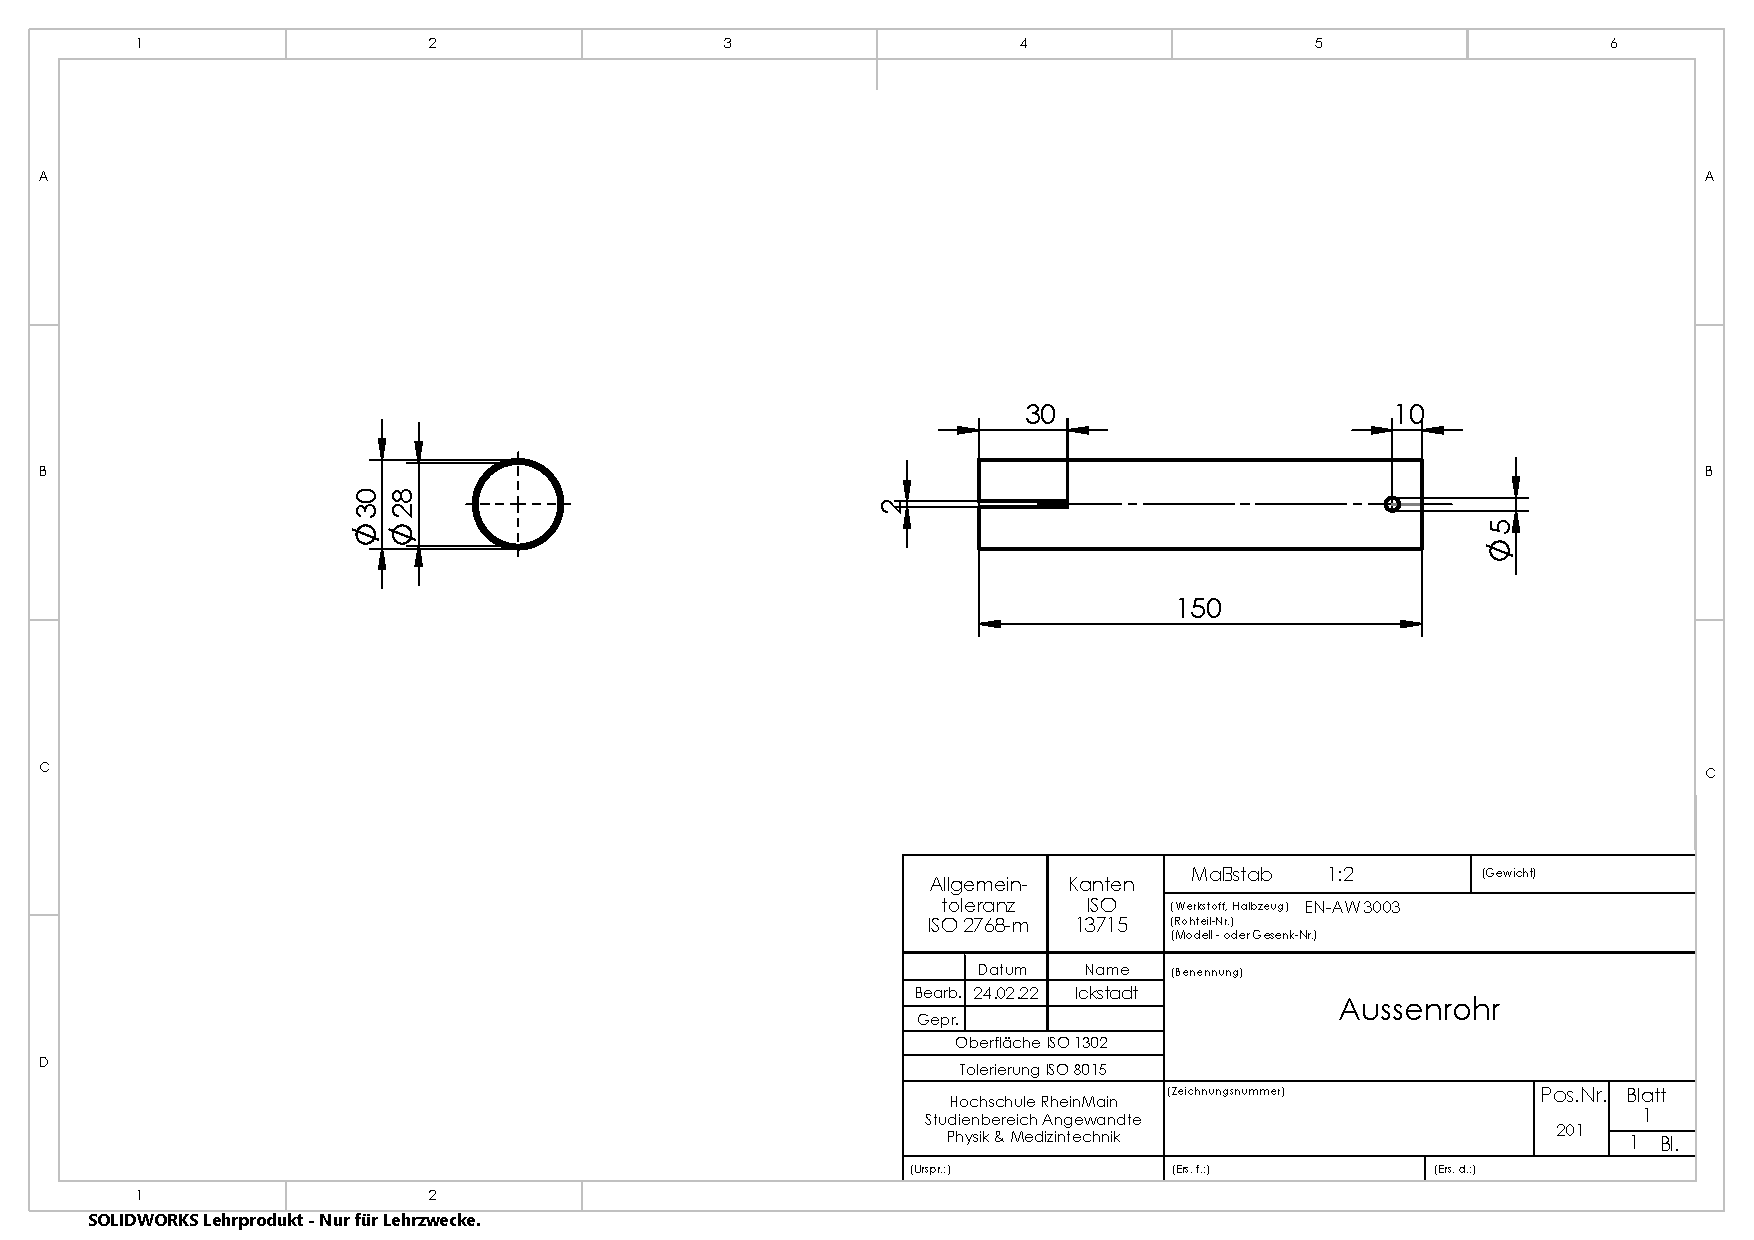
\includepdf[pages=-, angle=90, pagecommand={\thispagestyle{plain}}, addtolist={1, figure, Aussenrohr, drw:Aussenrohr}]{Abb/CAD/Drawings/Aussenrohr.pdf}
%
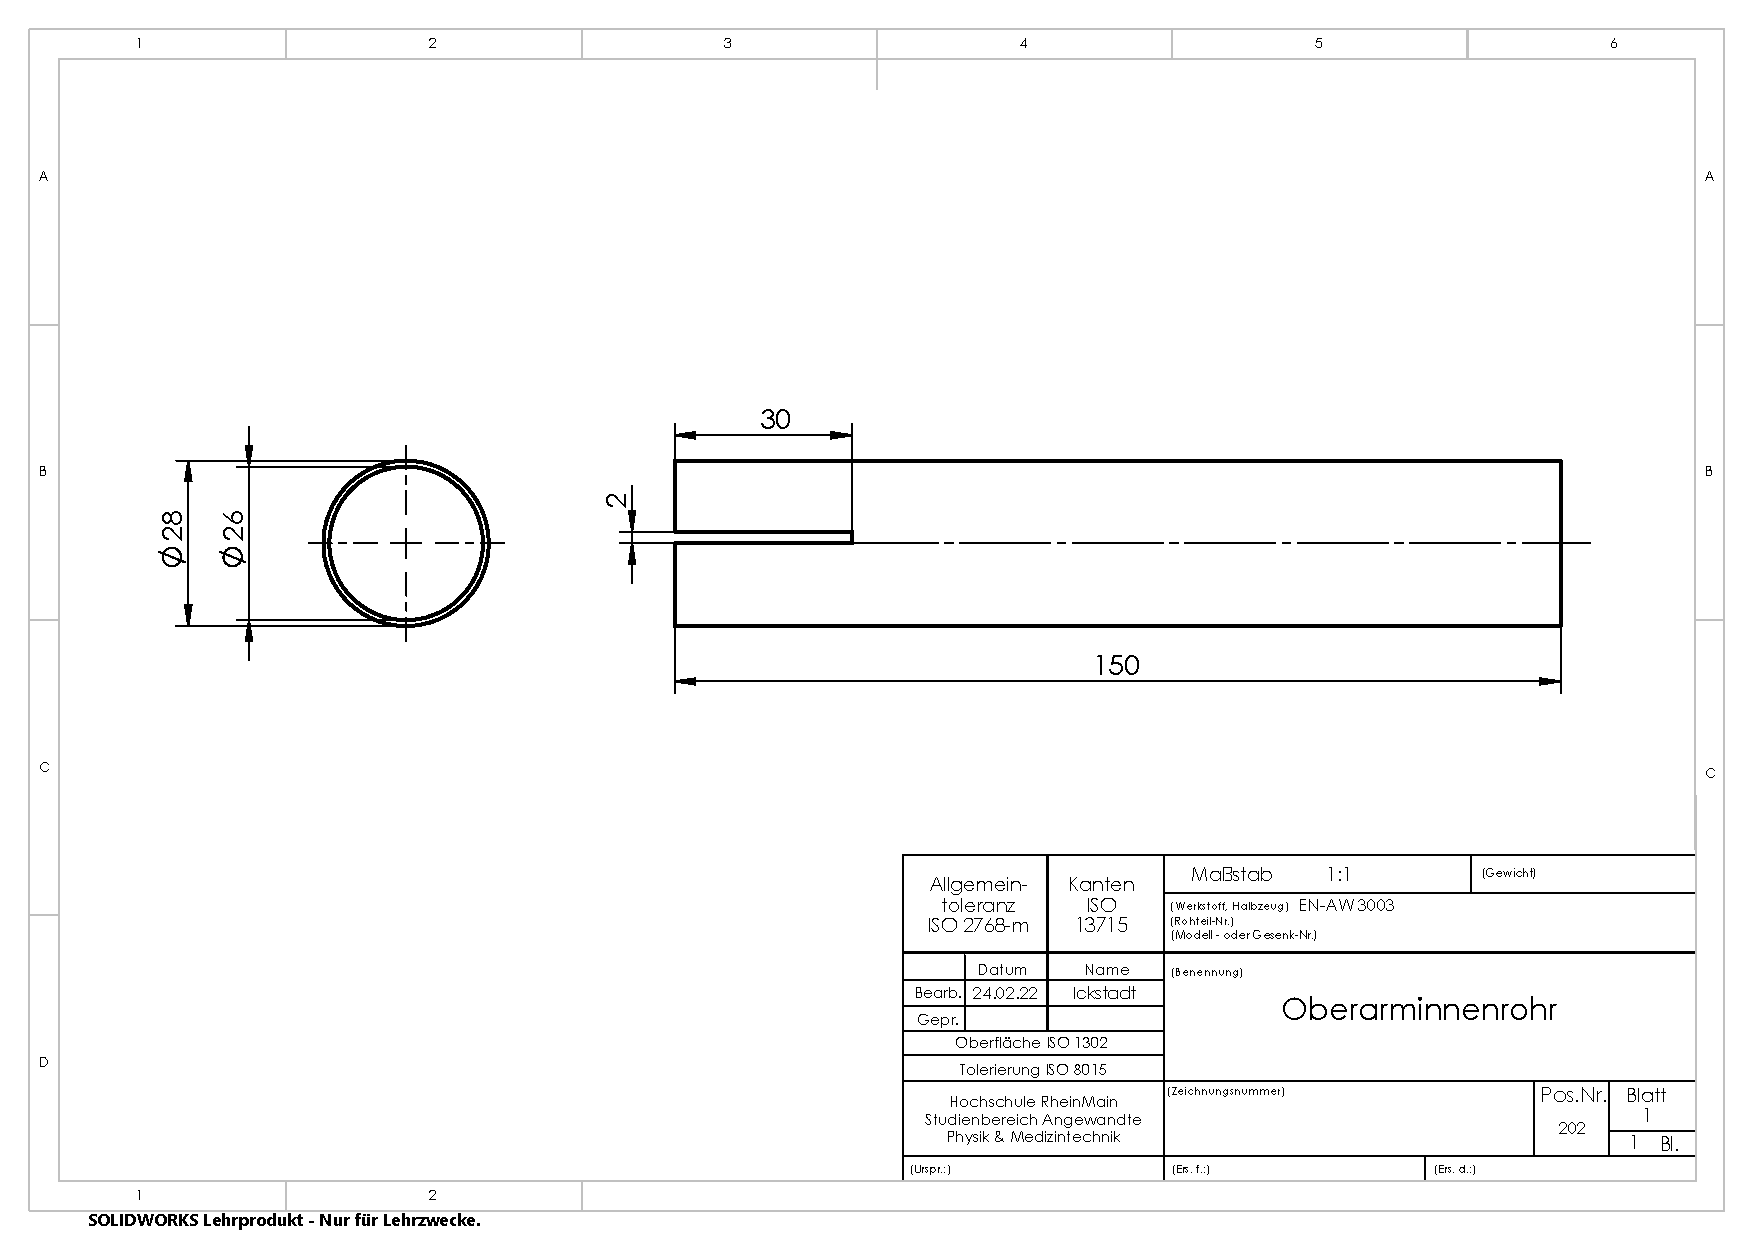
\includepdf[pages=-, angle=90, pagecommand={\thispagestyle{plain}}, addtolist={1, figure, Oberarminnenrohr, drw:Oberarminnenrohr}]{Abb/CAD/Drawings/Oberarminnenrohr.pdf}
%
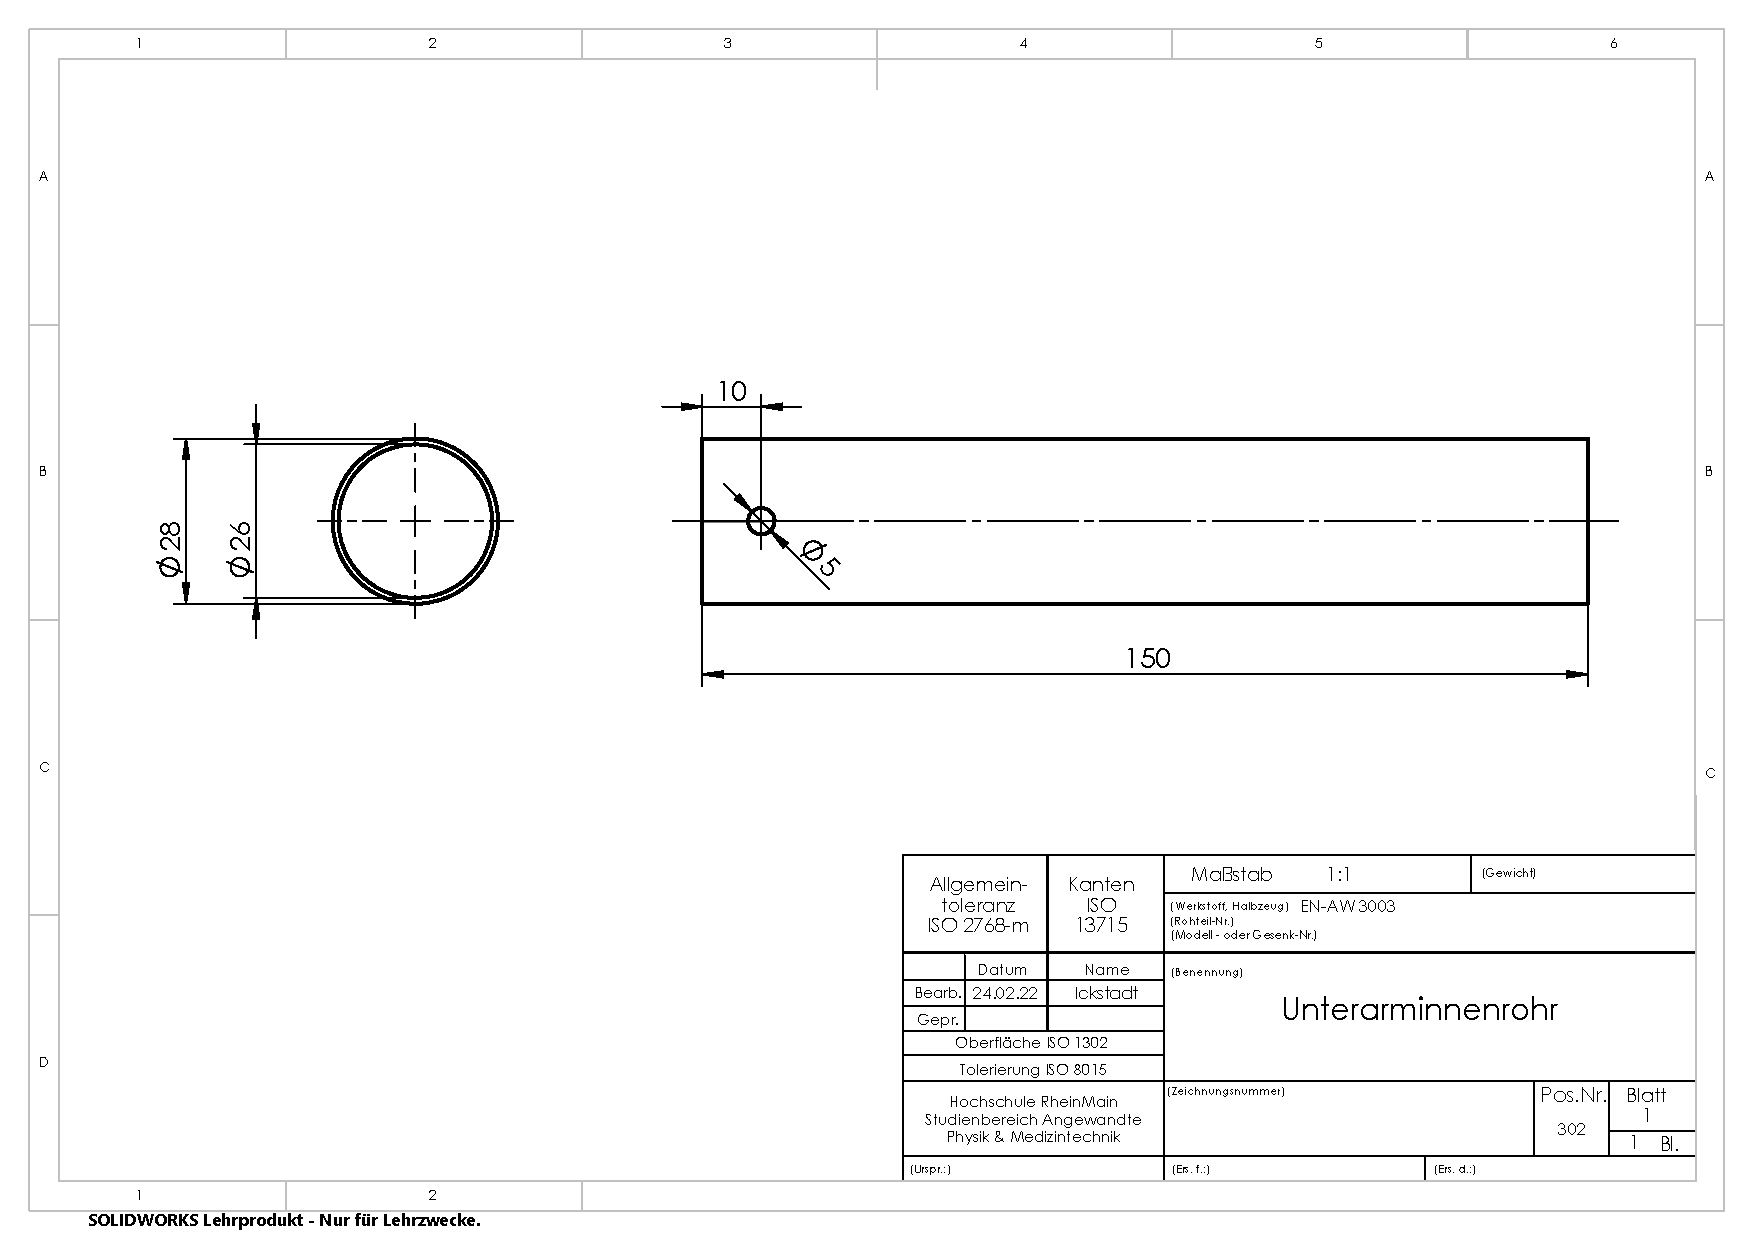
\includepdf[pages=-, angle=90, pagecommand={\thispagestyle{plain}}, addtolist={1, figure, Unterarminnenrohr, drw:Unterarminnenrohr}]{Abb/CAD/Drawings/Unterarminnenrohr.pdf}
%
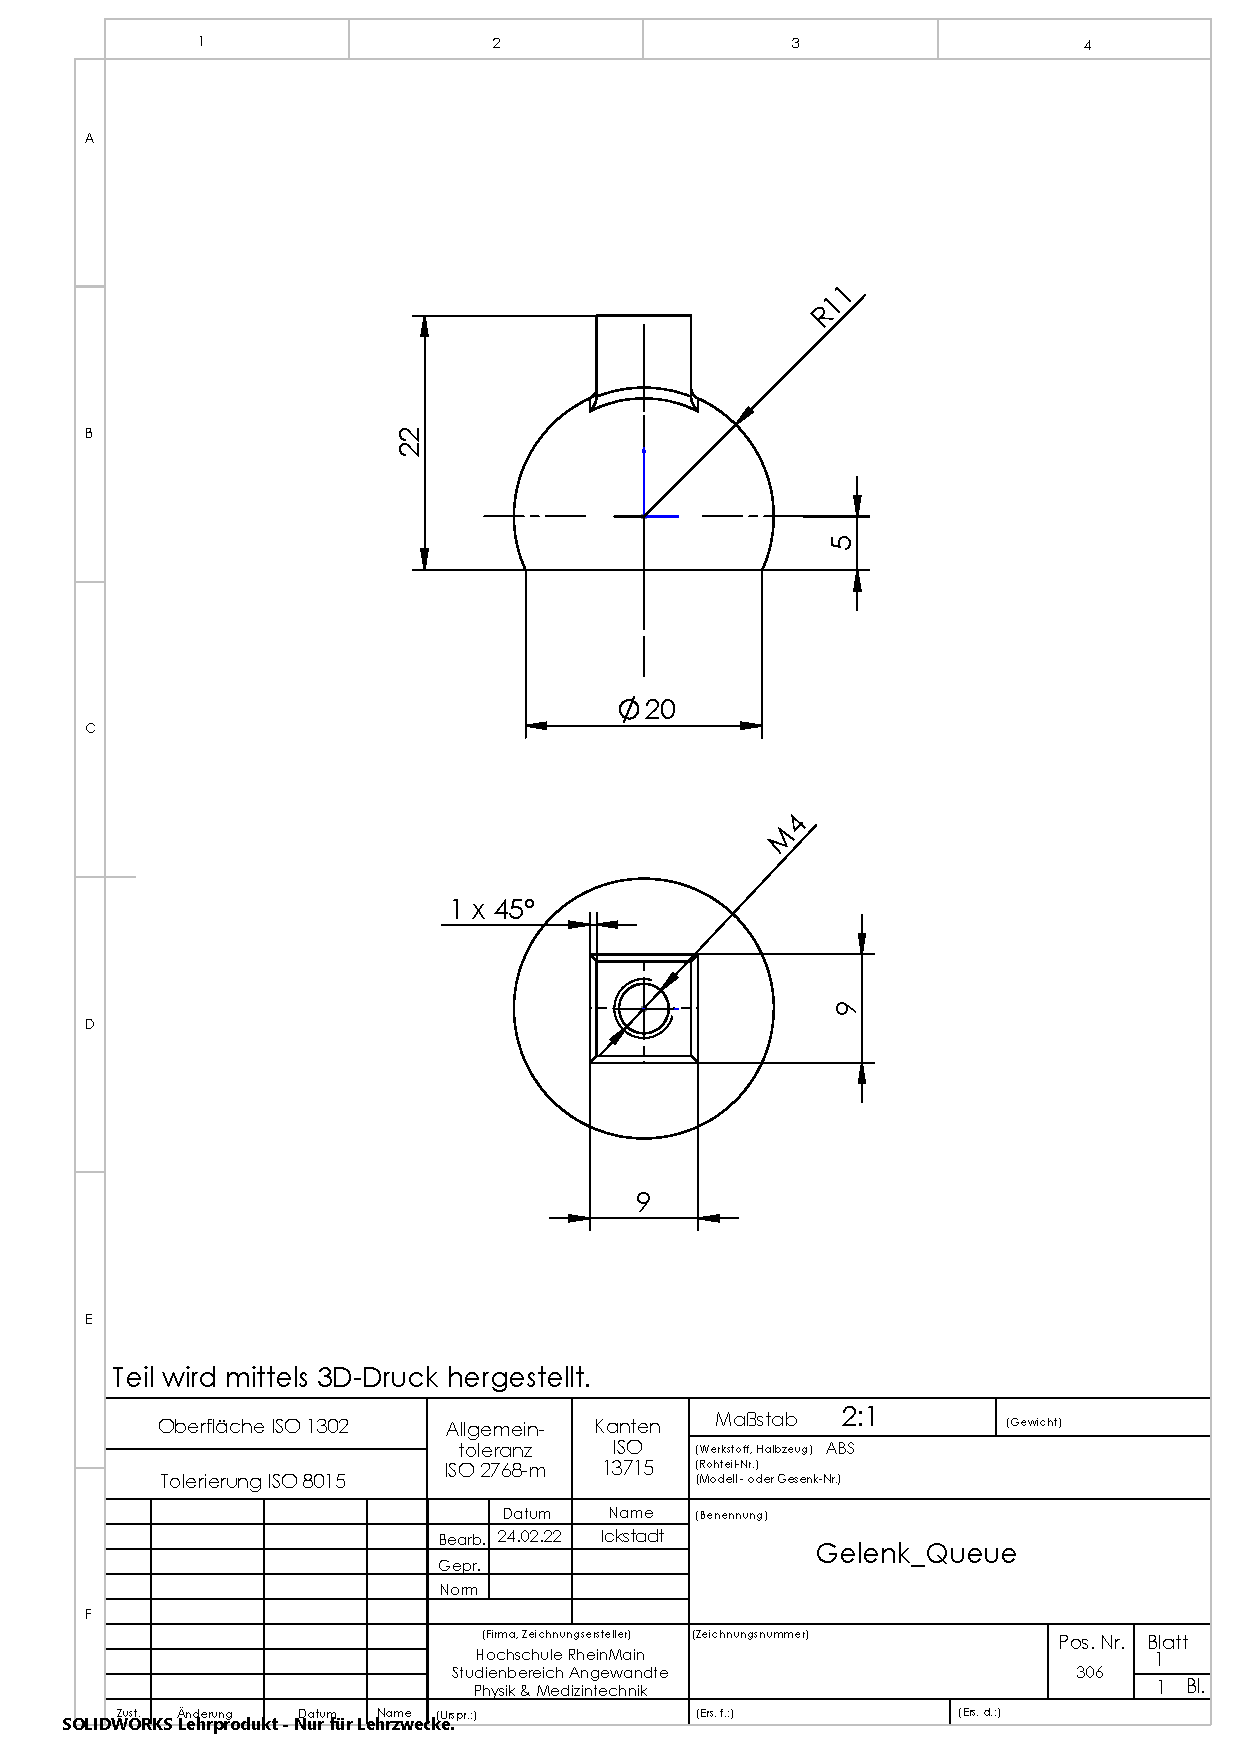
\includepdf[pages=-, angle=0, pagecommand={\thispagestyle{plain}}, addtolist={1, figure, Gelenk-Queue, drw:Gelenk-Queue}]{Abb/CAD/Drawings/Gelenk-Queue.pdf}
%
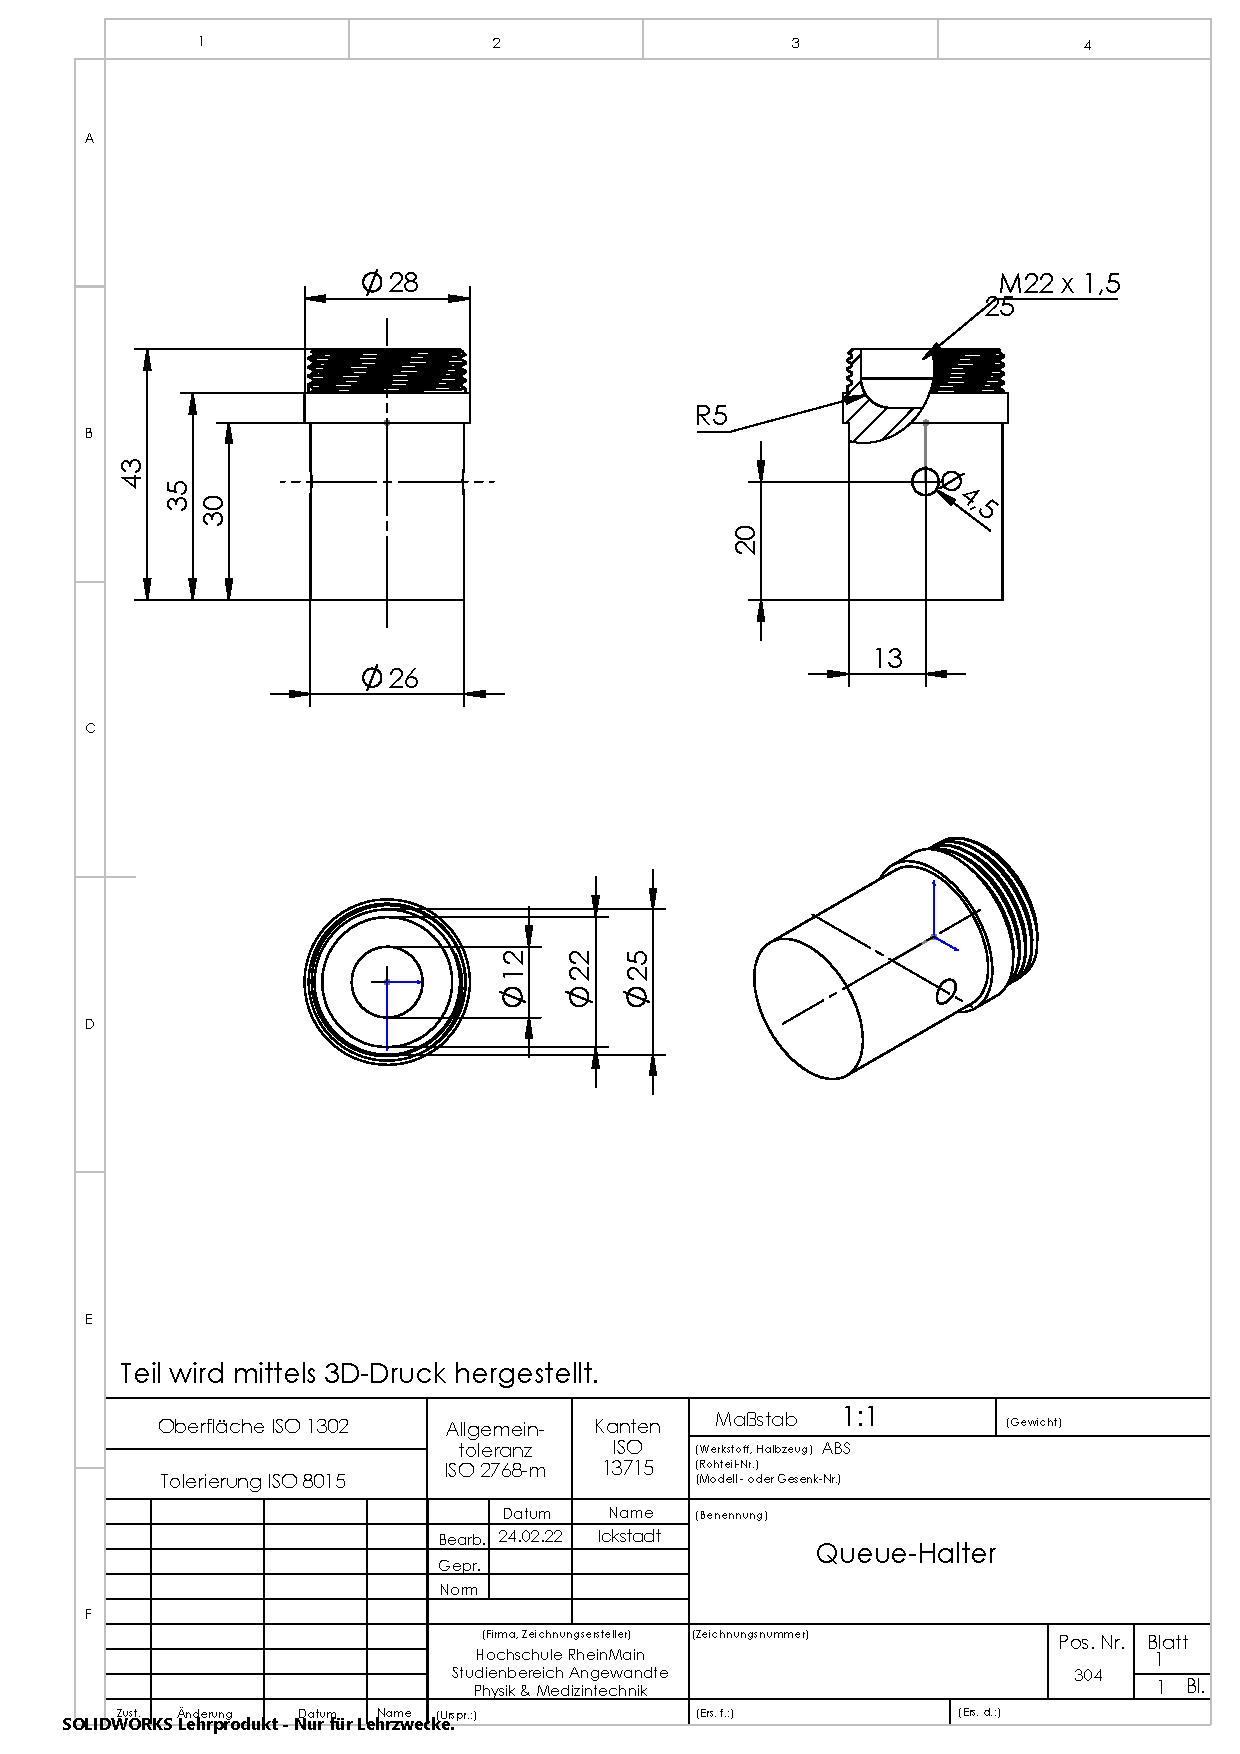
\includepdf[pages=-, angle=0, pagecommand={\thispagestyle{plain}}, addtolist={1, figure, Queue-Halter, drw:Queue-Halter}]{Abb/CAD/Drawings/Queue-Halter.pdf}
%
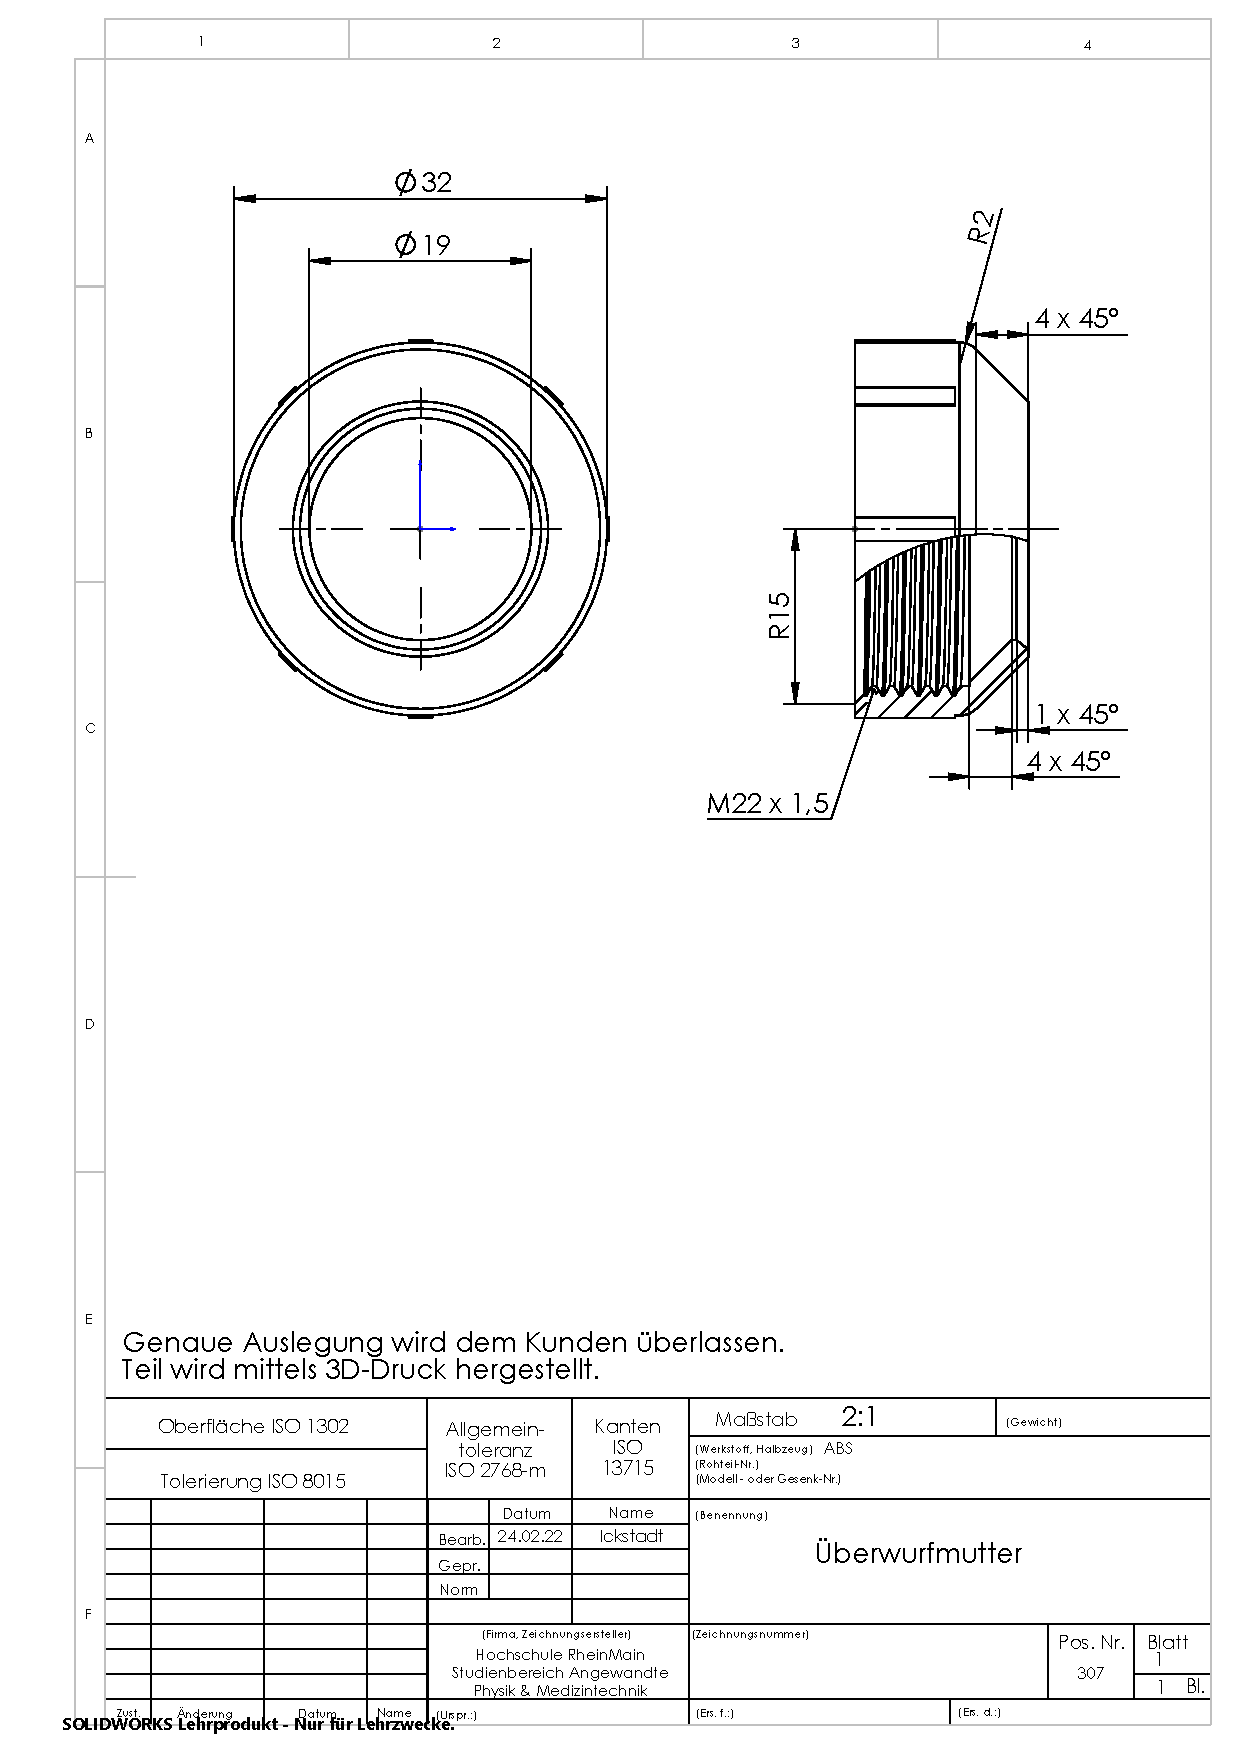
\includepdf[pages=-, angle=0, pagecommand={\thispagestyle{plain}}, addtolist={1, figure, Überwurfmutter, drw:Ueberwurfmutter}]{Abb/CAD/Drawings/Ueberwurfmutter.pdf}
%
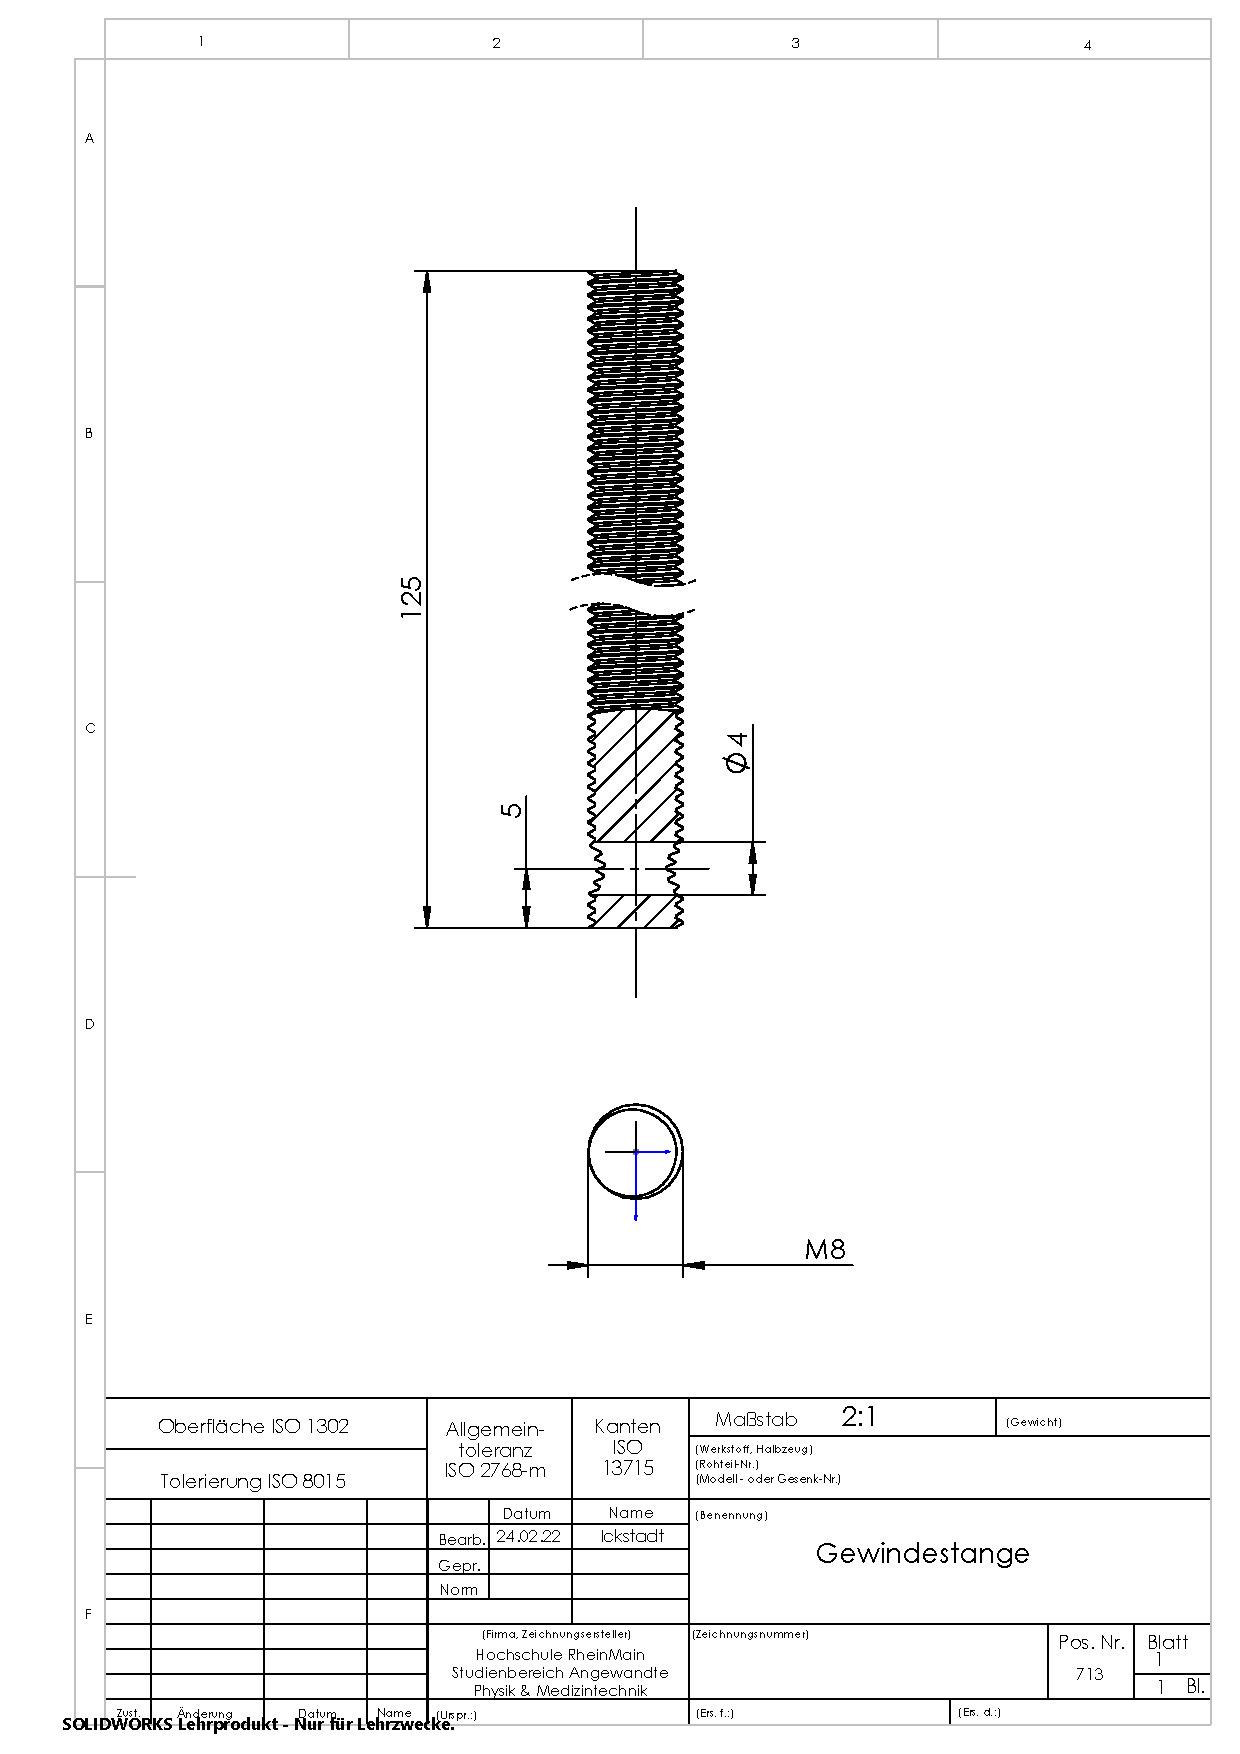
\includepdf[pages=-, angle=0, pagecommand={\thispagestyle{plain}}, addtolist={1, figure, Gewindestange, drw:Gewindestange}, addtotoc={1, section, 1, Einzelteilzeichnungen Ellbogengelenk, {sec:einzelteilzeichnungen ellbogengelenk}}]{Abb/CAD/Drawings/Gewindestange.pdf}
%
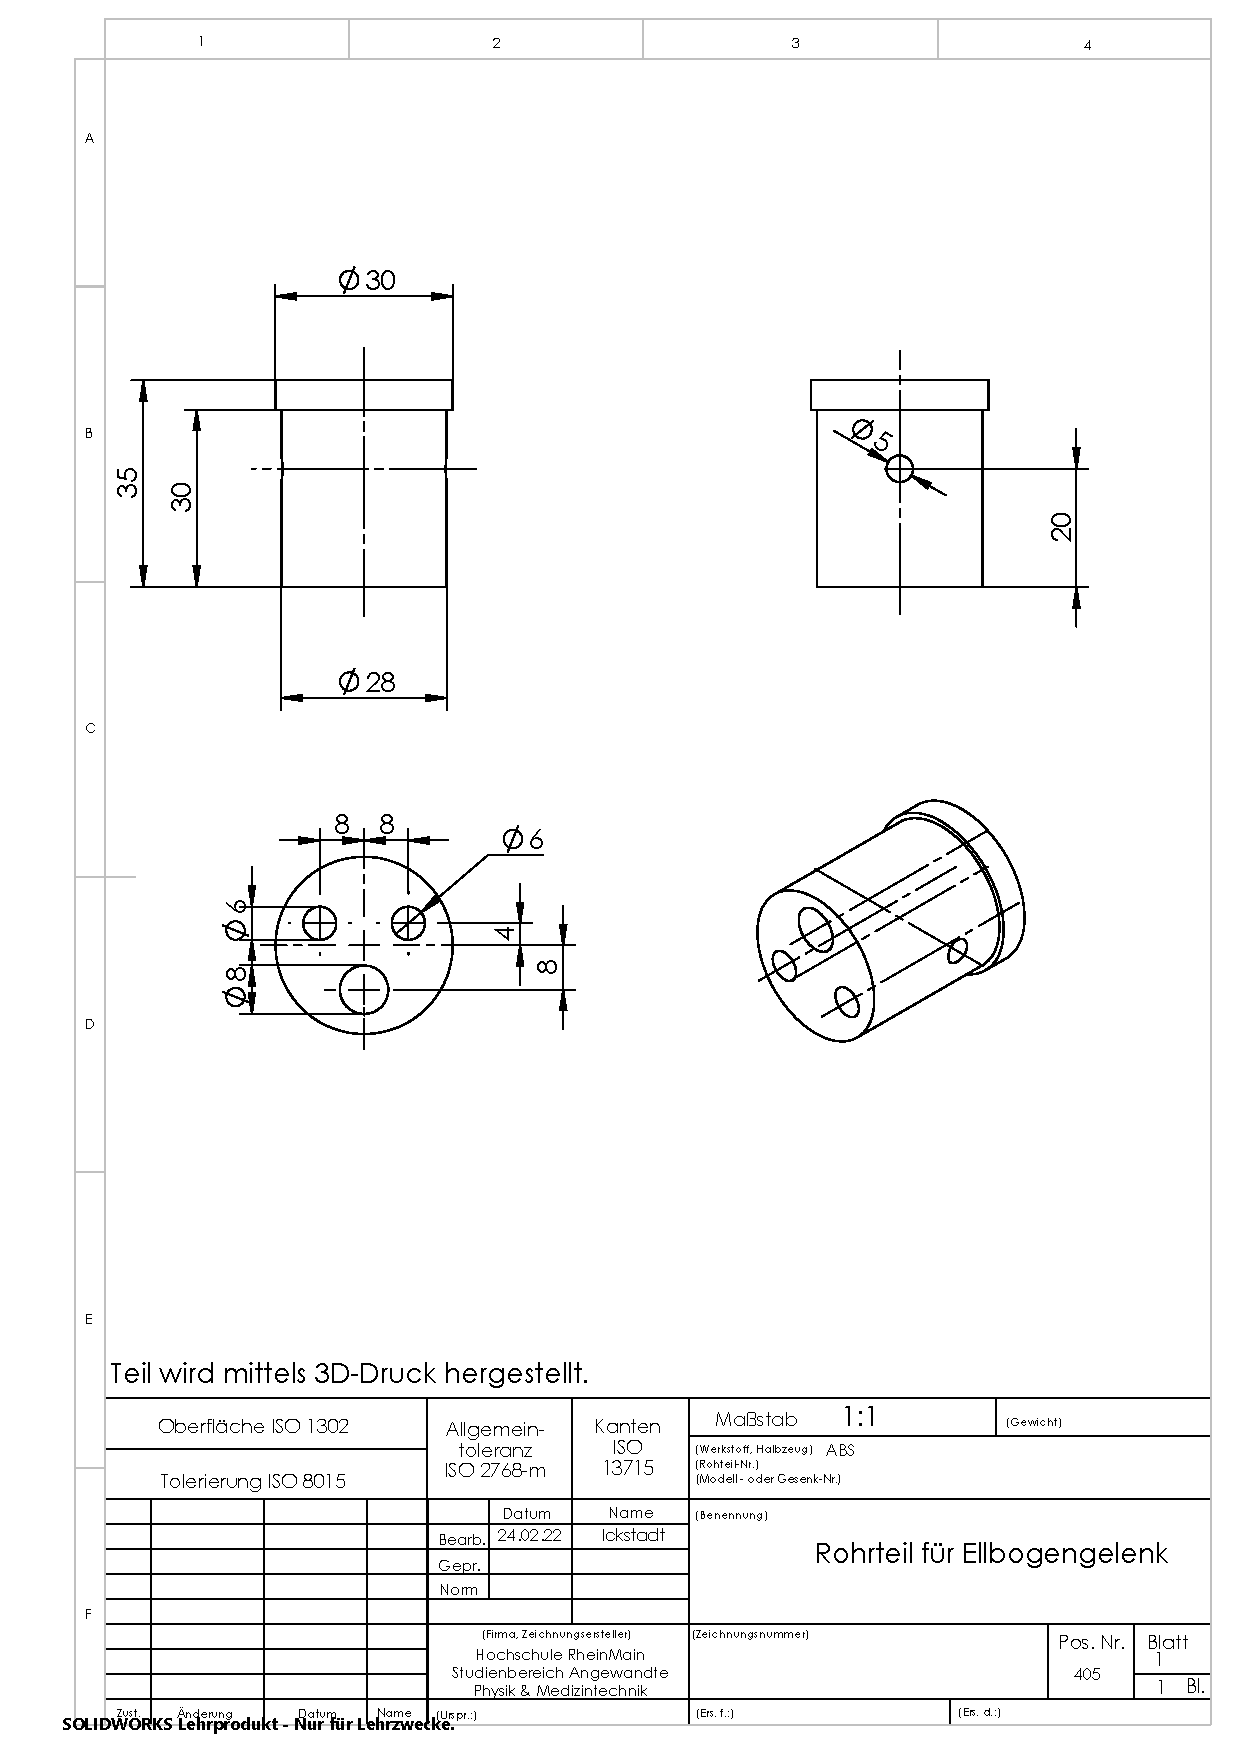
\includepdf[pages=-, angle=0, pagecommand={\thispagestyle{plain}}, addtolist={1, figure, Rohrteil für Ellbogengelenk, drw:Rohrteil-fuer-Ellbogengelenk}]{Abb/CAD/Drawings/Rohrteil-fuer-Ellbogengelenk.pdf}
%
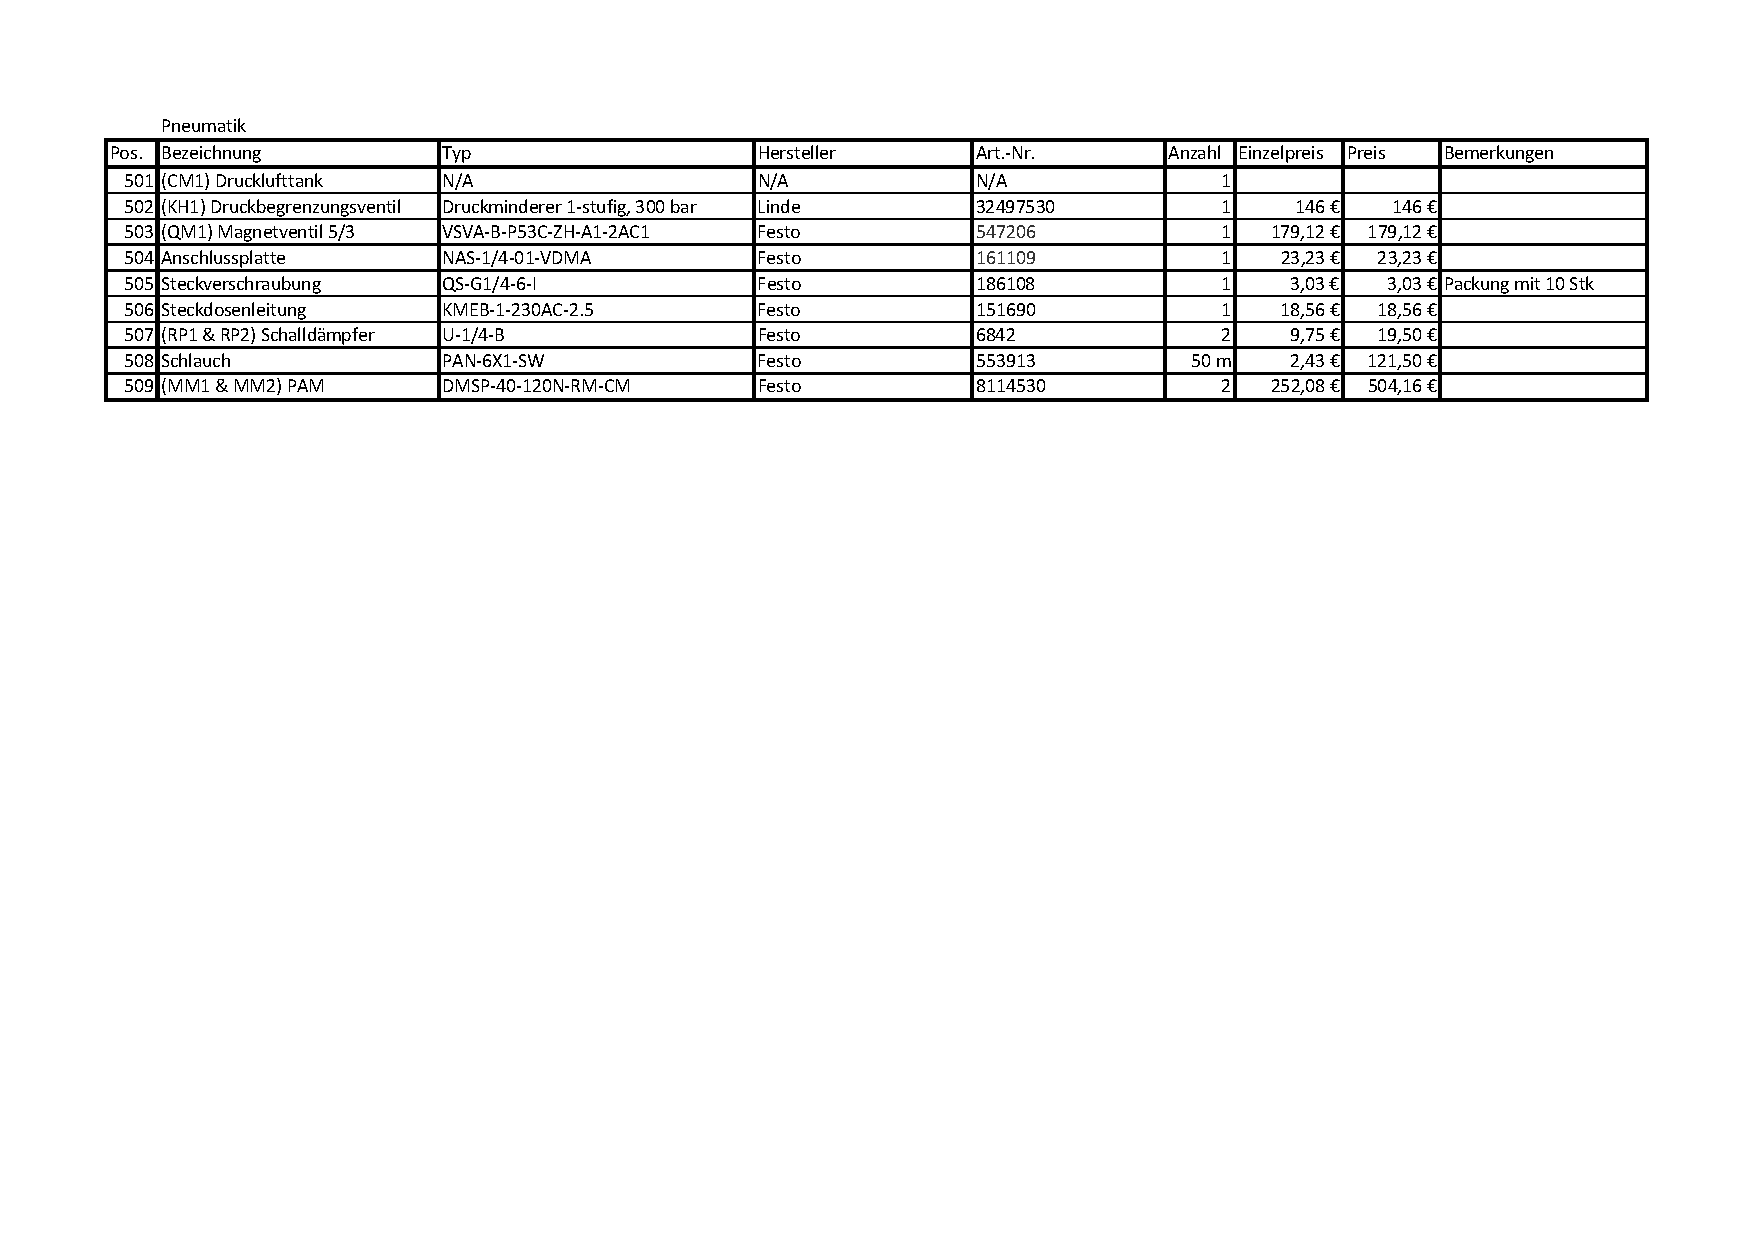
\includepdf[pages=-, angle=90, pagecommand={\thispagestyle{plain}}, addtolist={1, table, Stückliste Pneumatik, tab:StuecklistePneumatik}, addtotoc={1, section, 1, Generelle Stückliste und Pneumatikschaltplan, sec:stueckliste und pneumatikschaltplan}]{Abb/Stuecklisten/StuecklistePneumatik.pdf}
%
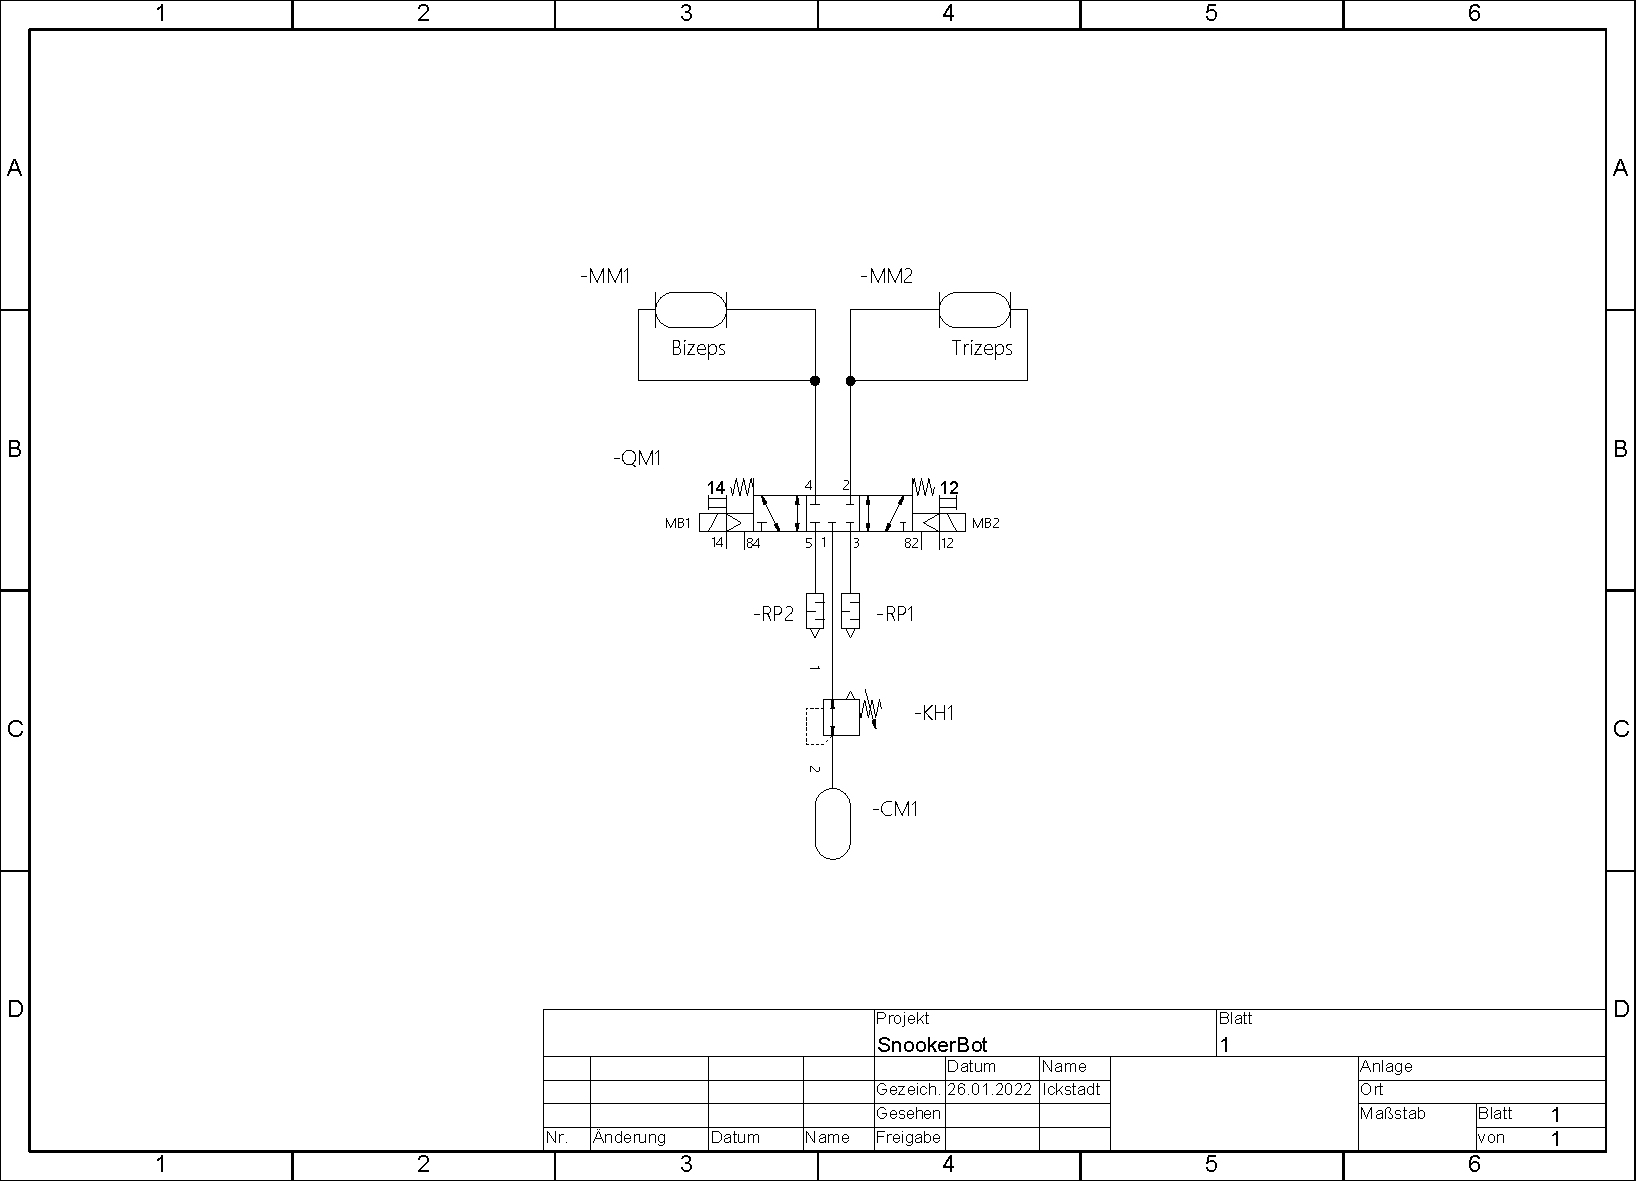
\includepdf[pages=-, angle=90, pagecommand={\thispagestyle{plain}}, addtolist={1, figure, Pneumatikschaltplan, drw:PneumatikZeichnung}]{Abb/PneumatikZeichnung.pdf}
%
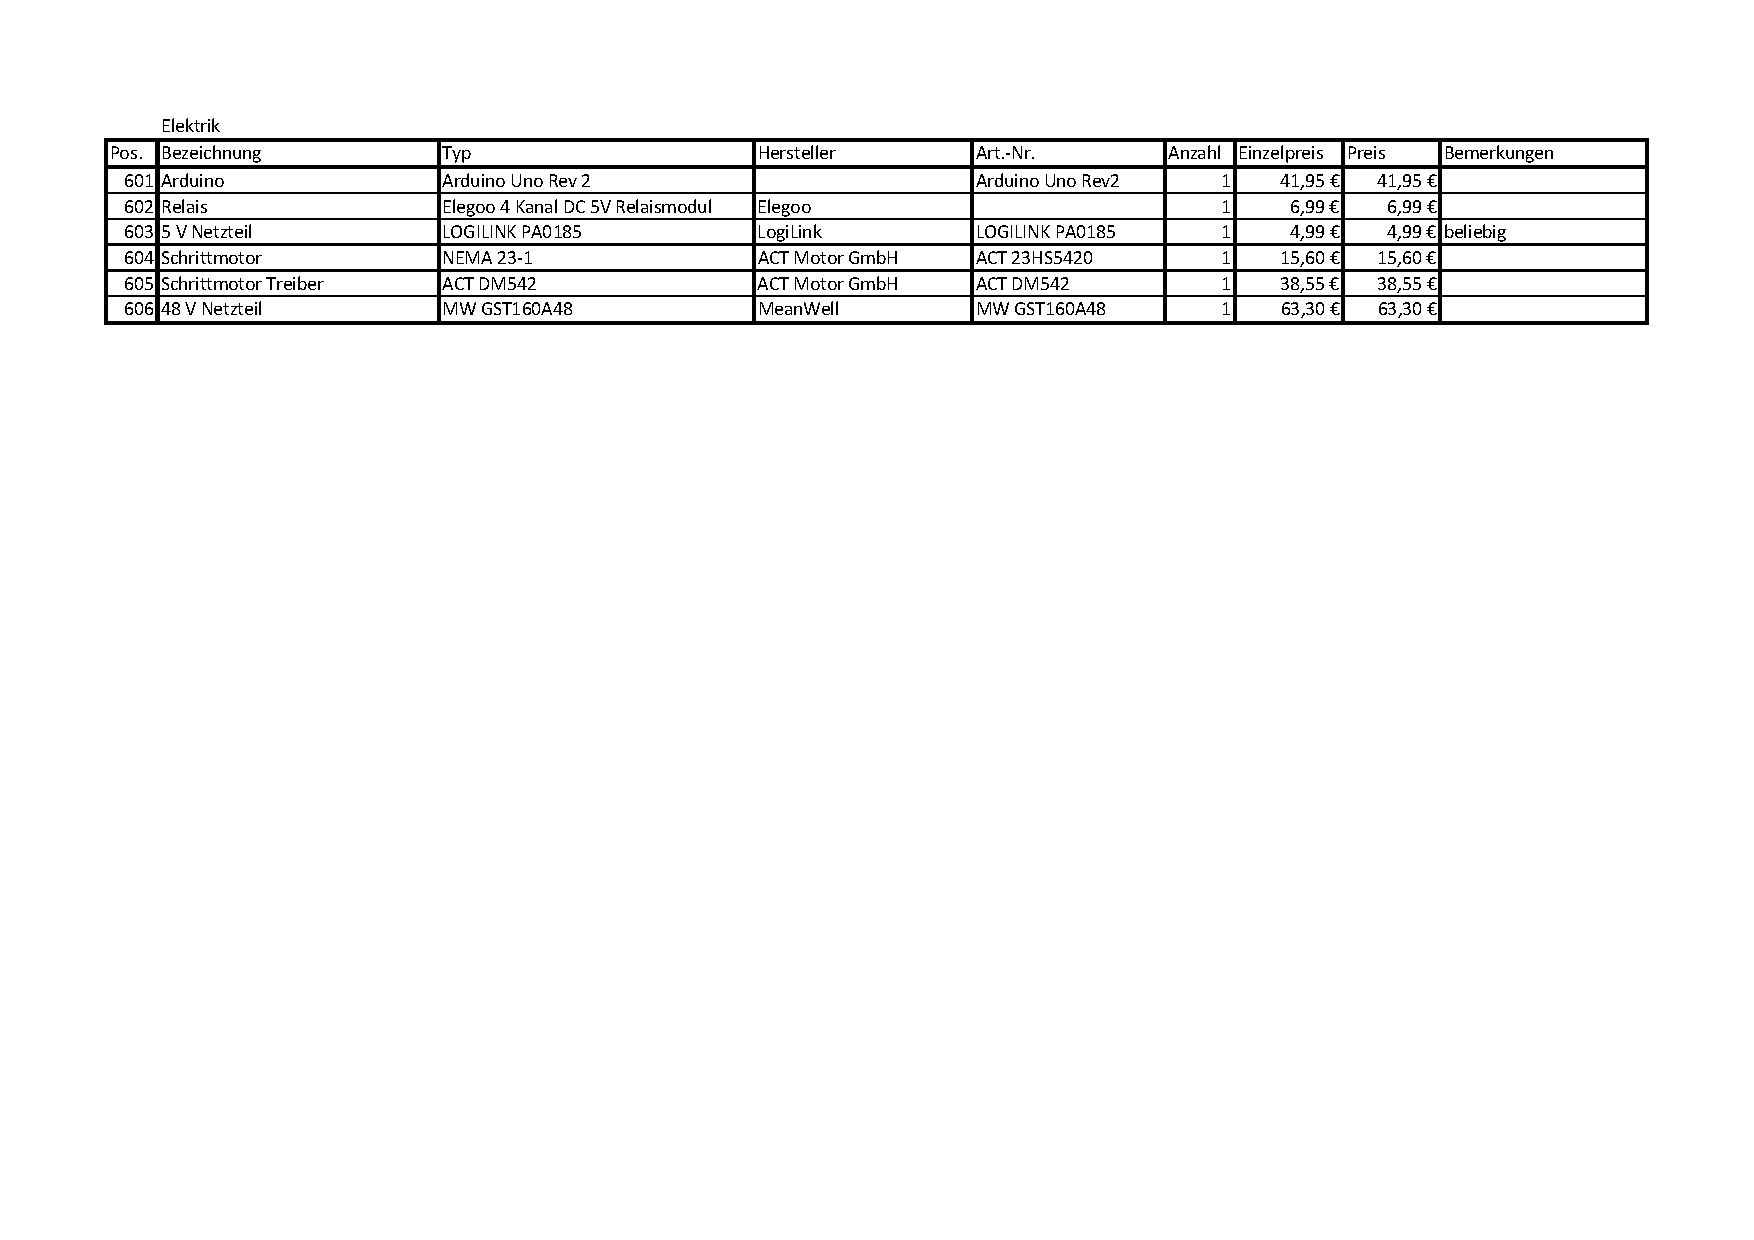
\includepdf[pages=-, angle=90, pagecommand={\thispagestyle{plain}}, addtolist={1, table, Stückliste Elektrik, tab:StuecklisteElektrik}]{Abb/Stuecklisten/StuecklisteElektrik.pdf}
%
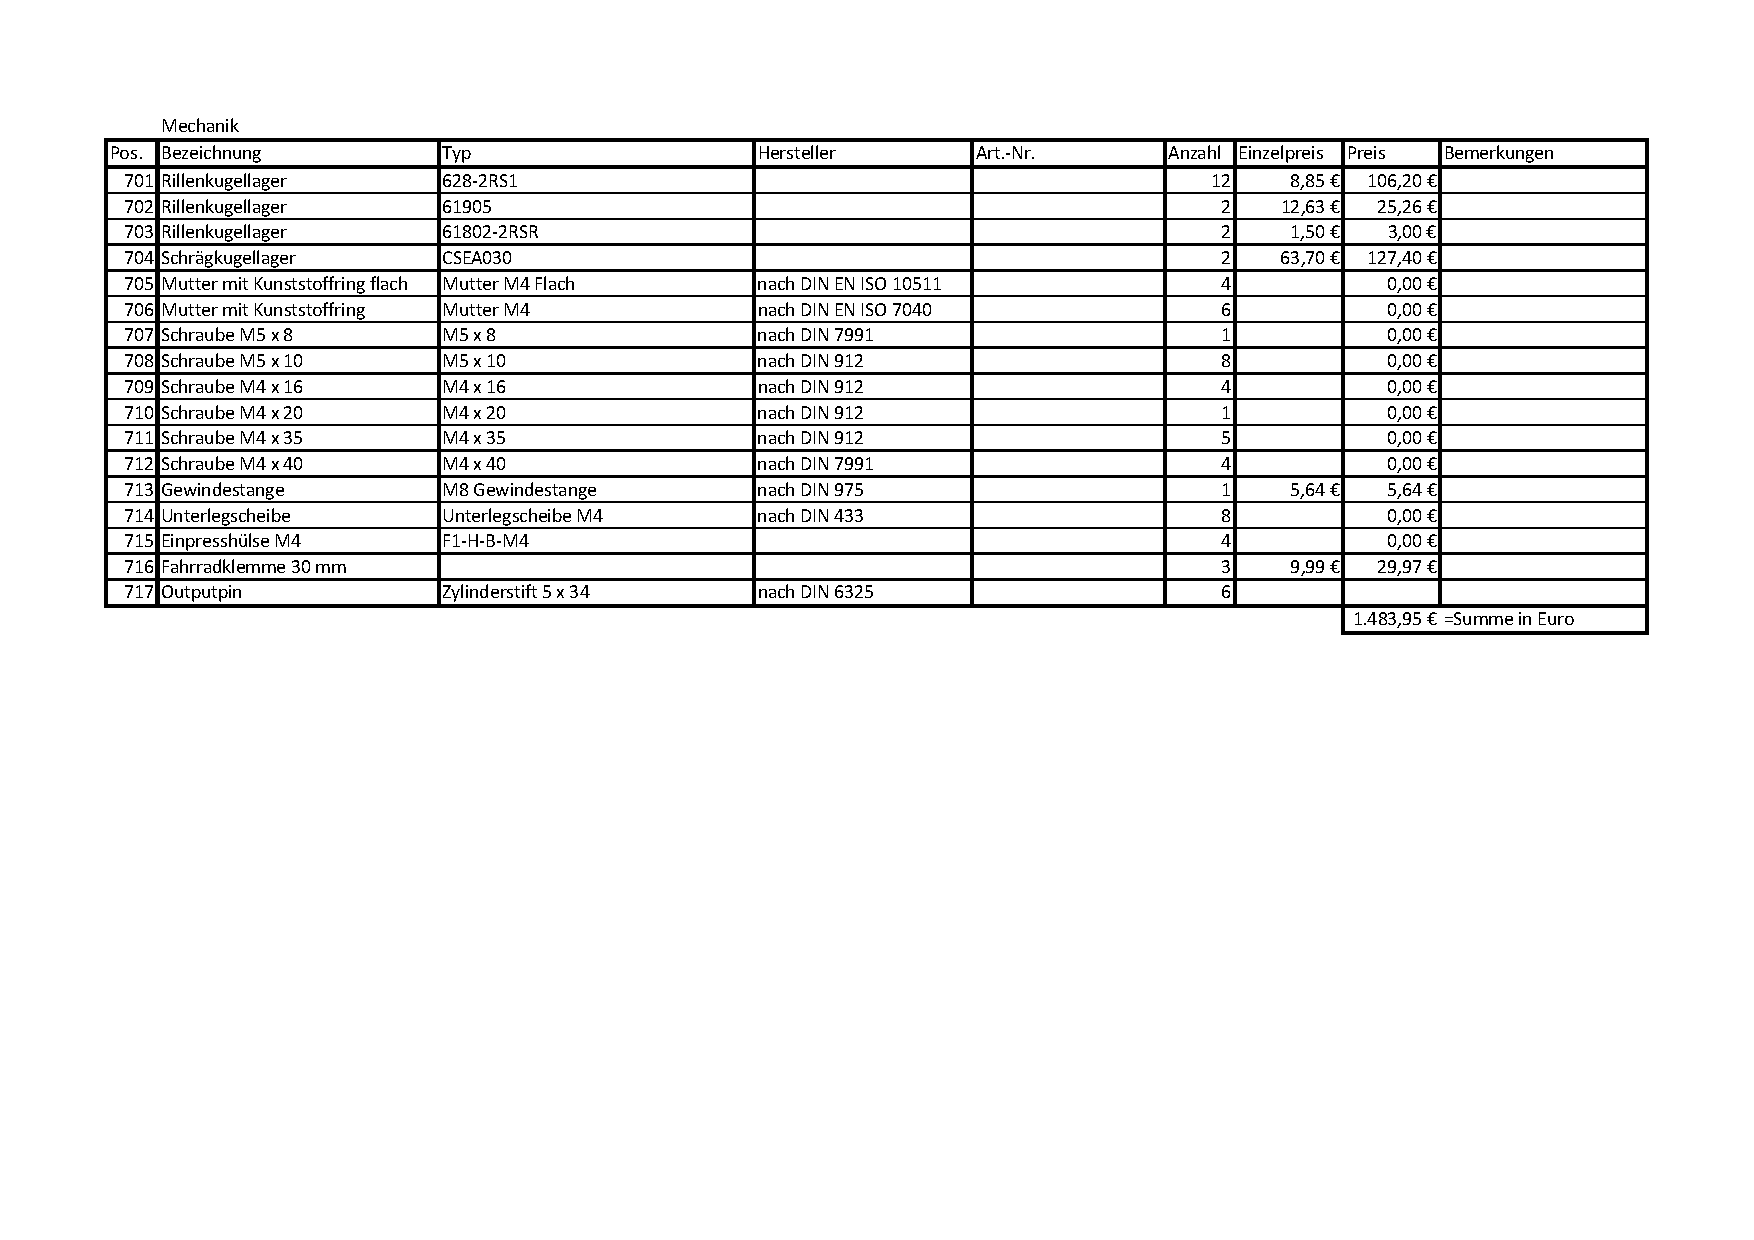
\includepdf[pages=-, angle=90, pagecommand={\thispagestyle{plain}}, addtolist={1, table, Stückliste Mechanik, tab:StuecklisteMech}]{Abb/Stuecklisten/StuecklisteMech.pdf}
\newpage
\setlength{\voffset}{-2.5 cm}
\setlength{\hoffset}{-2 cm}
\chapter{Zeichnungen}\label{sec:zeichnungen}
\newpage
\setlength{\voffset}{0cm}
\setlength{\hoffset}{0cm}
%
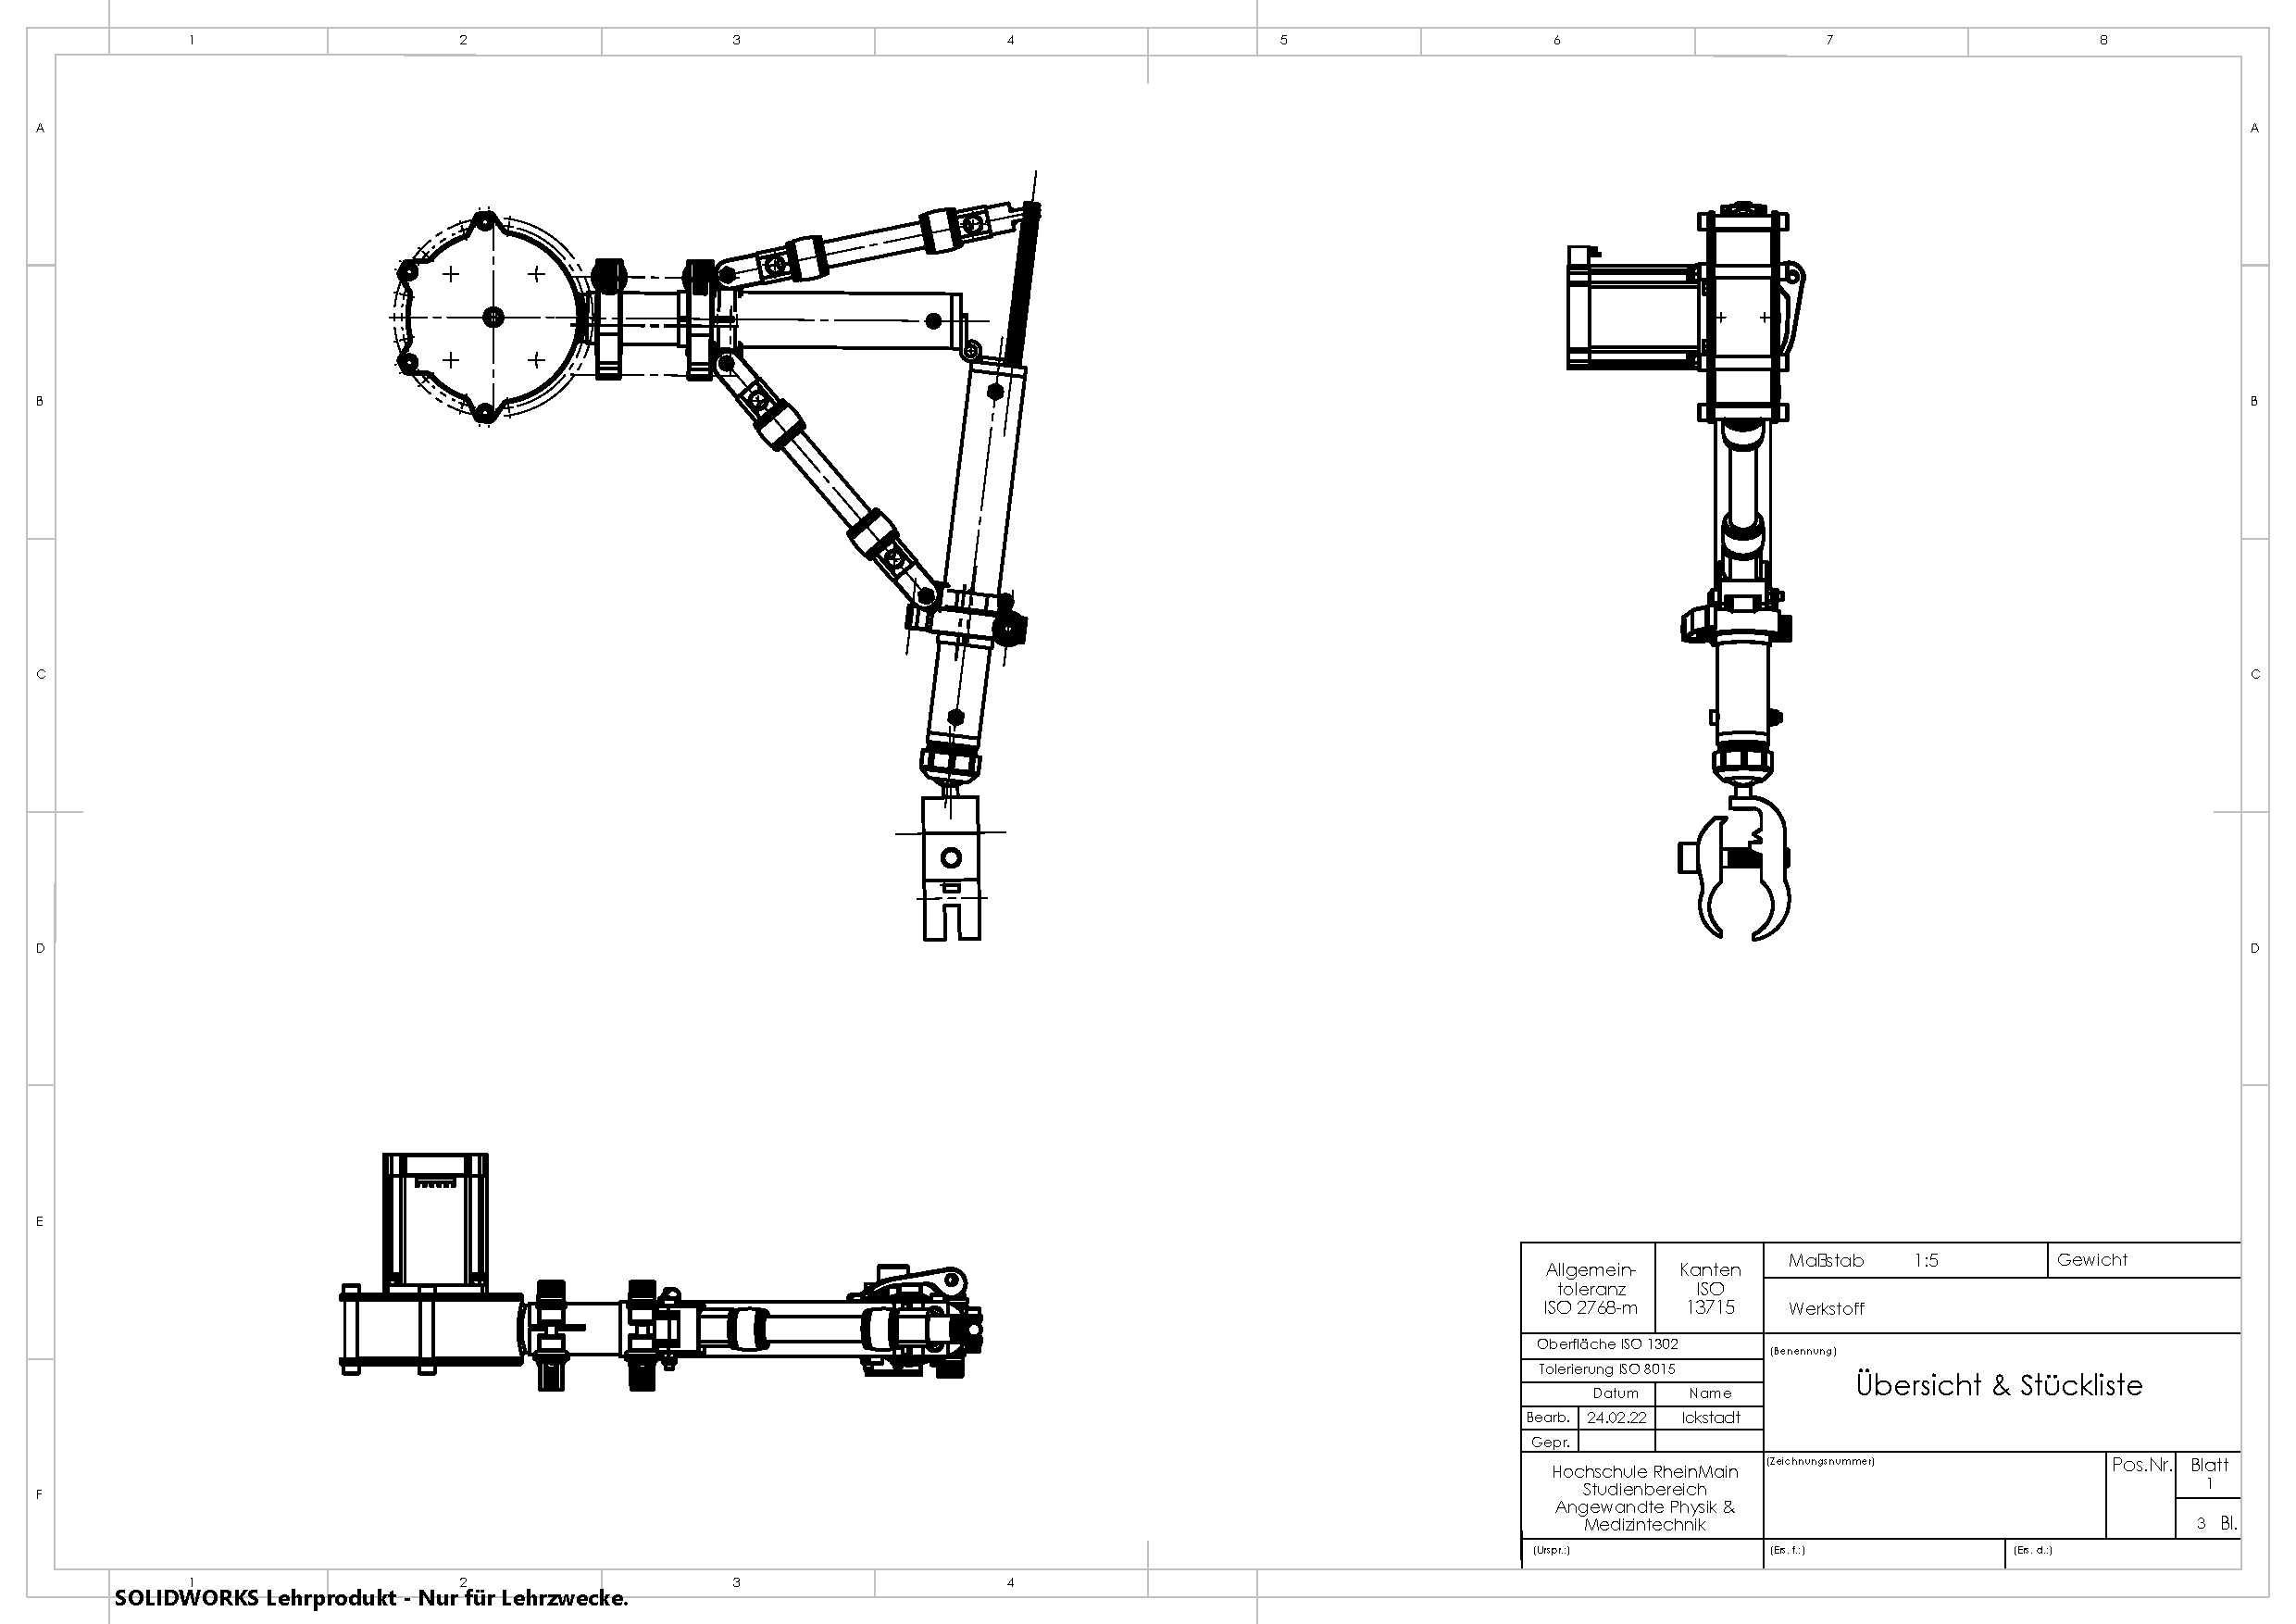
\includepdf[pages=1, angle=90, pagecommand={\thispagestyle{plain}}, addtolist={1, figure, Übersicht und Stückliste, drw:Uebersicht und Stueckliste}, addtotoc={1, section, 1, Bauteilzeichnungen, sec:bauteilzeichnungen}]{Abb/CAD/Drawings/Uebersicht-und-Stueckliste.pdf}
\includepdf[pages=2, angle=90, pagecommand={\thispagestyle{plain}}]{Abb/CAD/Drawings/Uebersicht-und-Stueckliste.pdf}
%
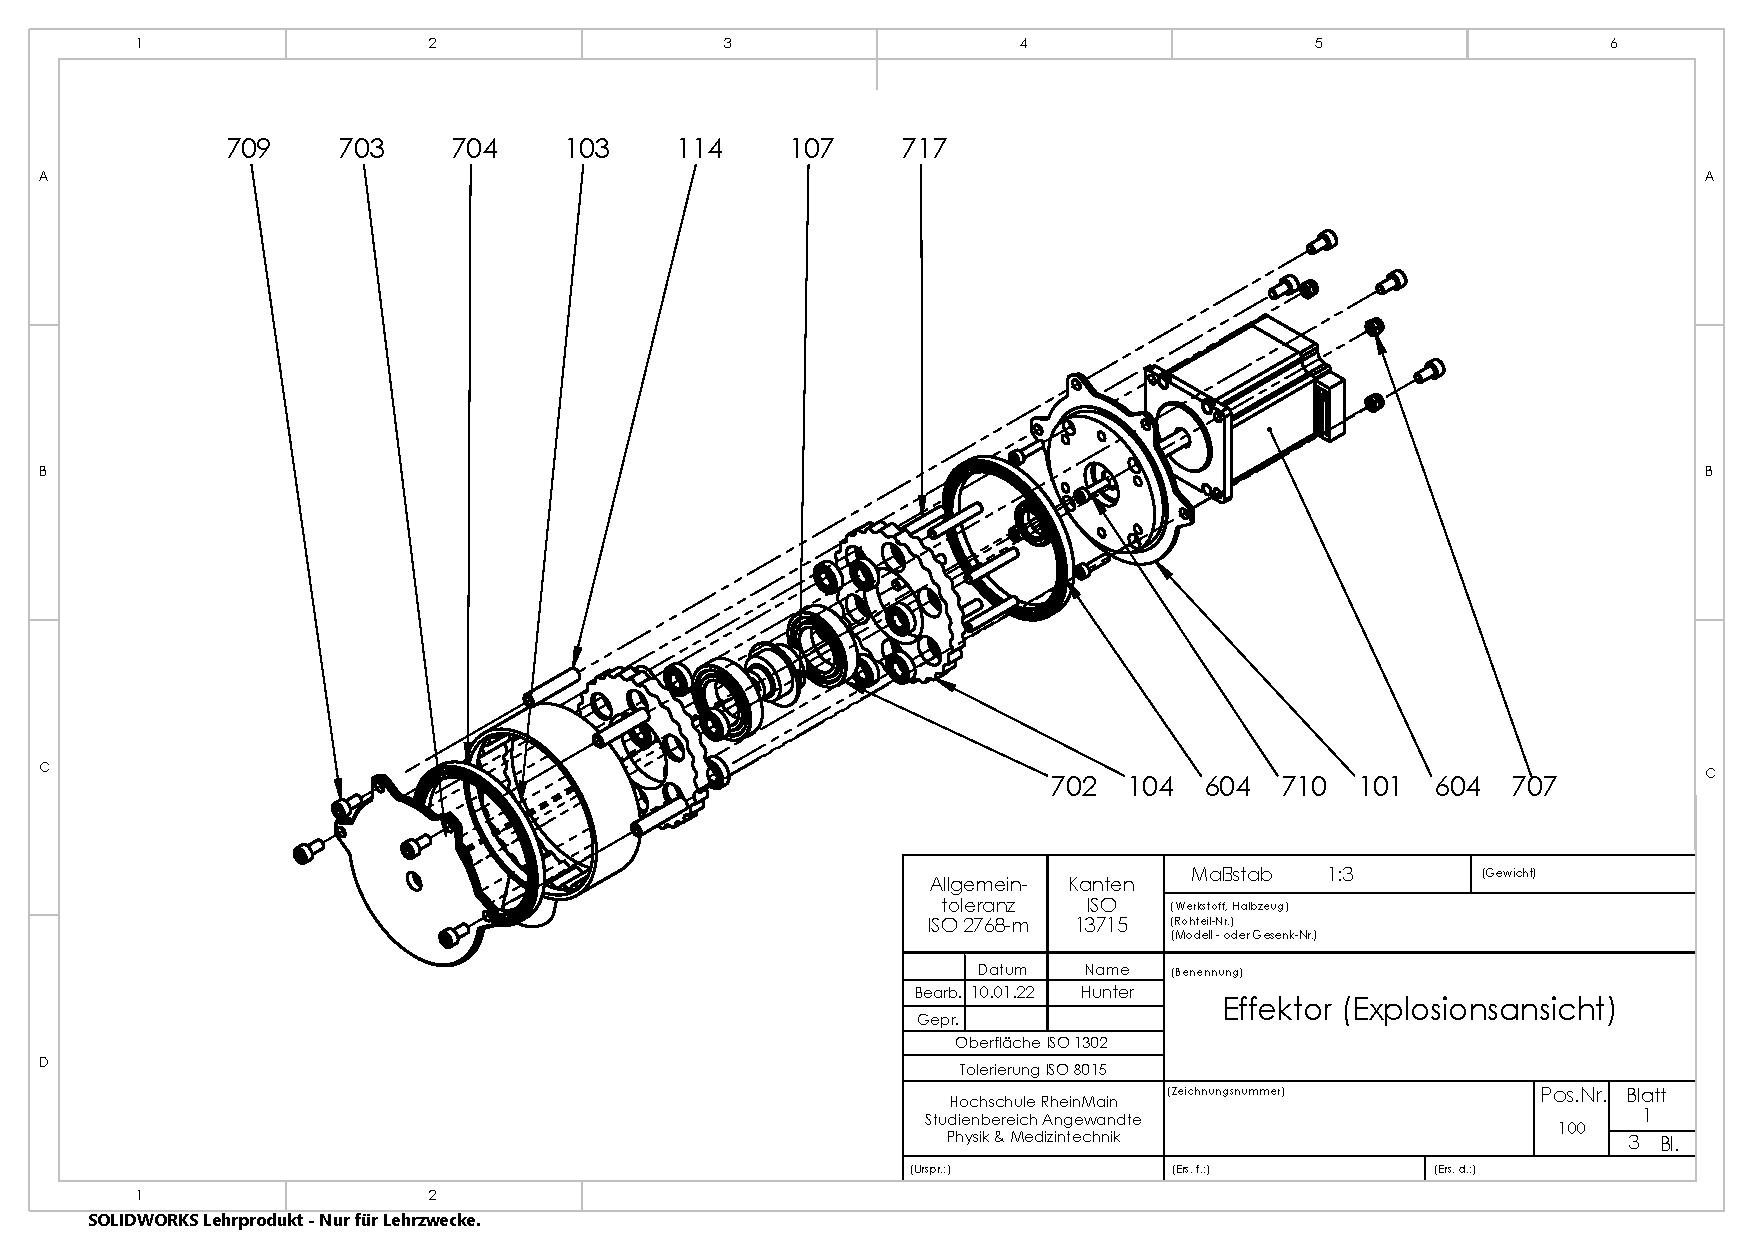
\includepdf[pages=1, angle=90, pagecommand={\thispagestyle{plain}}, addtolist={1, figure, Effektor, drw:Effektor}]{Abb/CAD/Drawings/Schulter/Effektor-assembly-drawing.pdf}
\includepdf[pages=2-3, angle=0, pagecommand={\thispagestyle{plain}}]{Abb/CAD/Drawings/Schulter/Effektor-assembly-drawing.pdf}
%
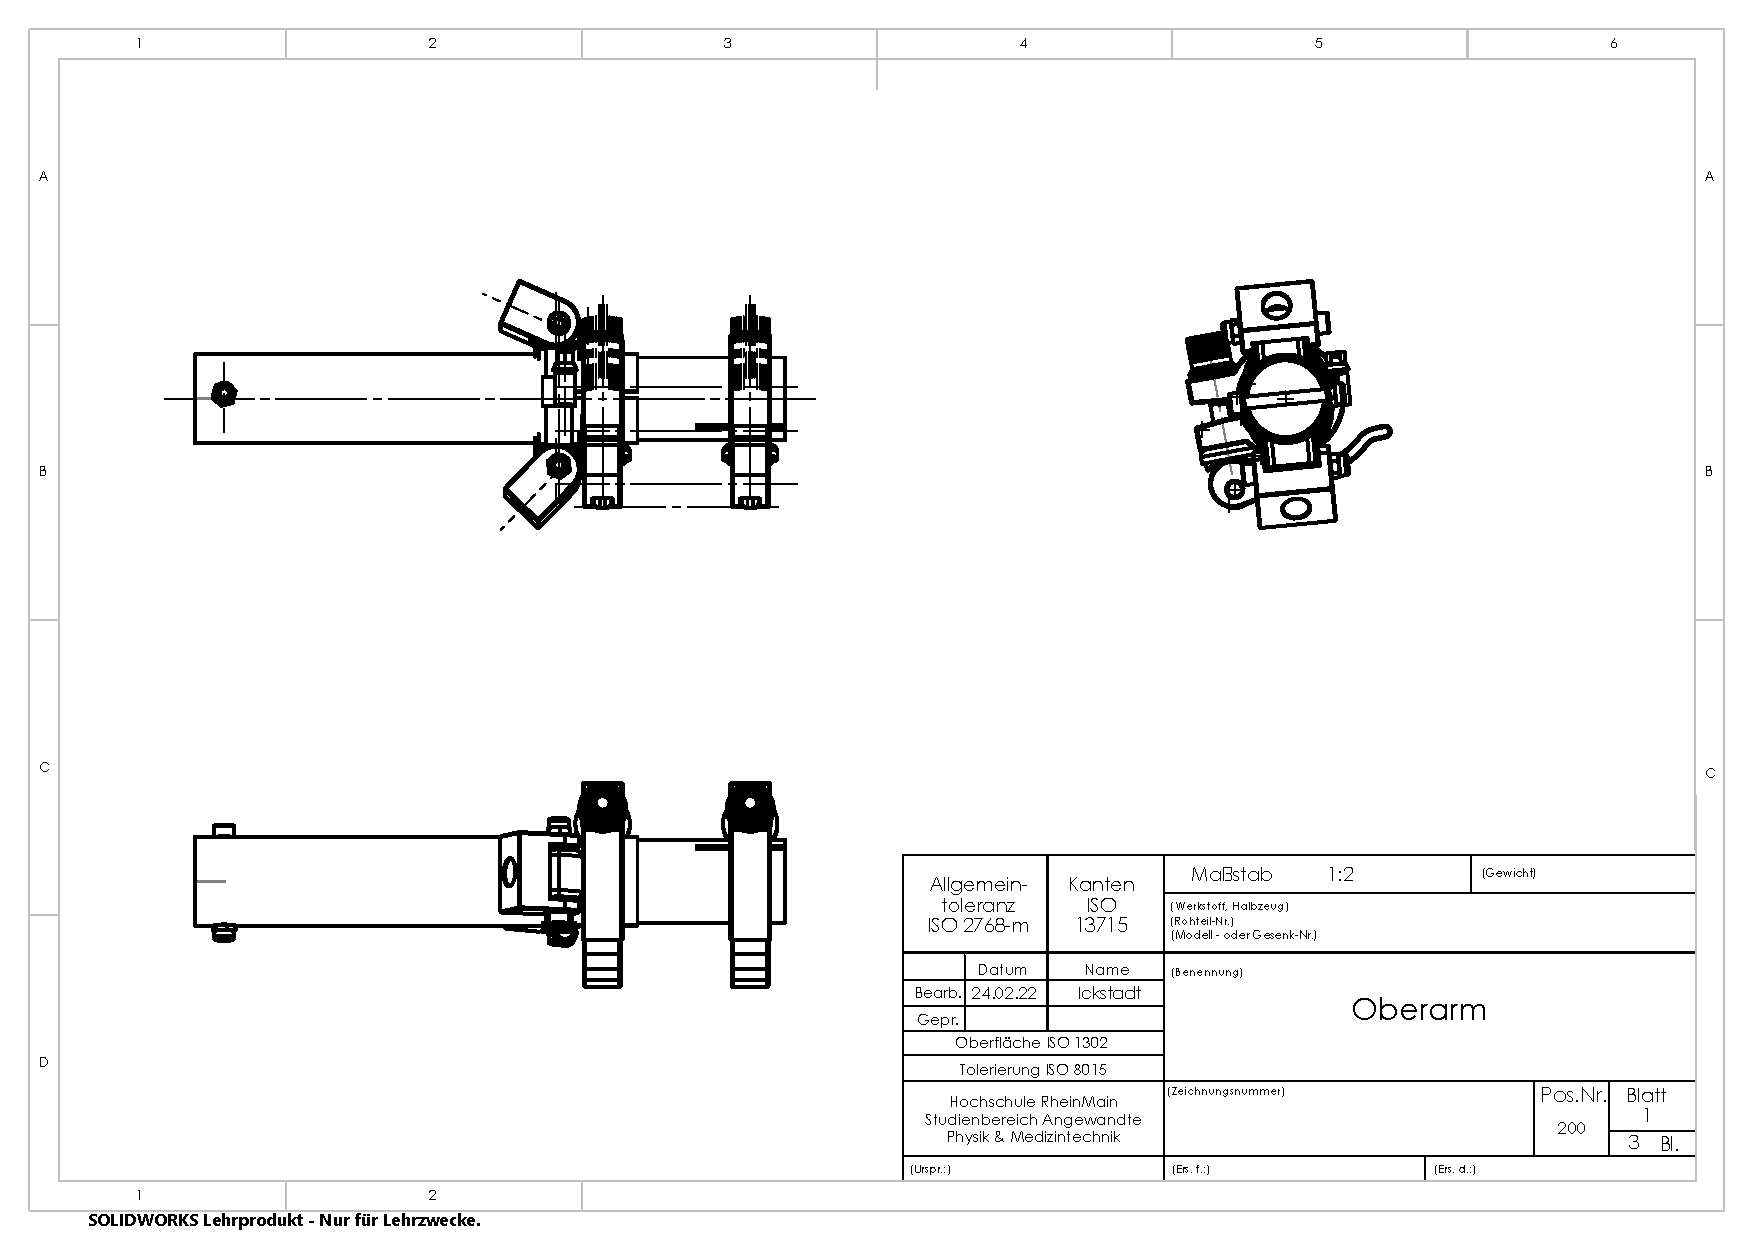
\includepdf[pages=1-2, angle=90, pagecommand={\thispagestyle{plain}}, addtolist={1, figure, Oberarm, drw:Oberarm}]{Abb/CAD/Drawings/Oberarm.pdf}
\includepdf[pages=3, angle=0, pagecommand={\thispagestyle{plain}}]{Abb/CAD/Drawings/Oberarm.pdf}
%
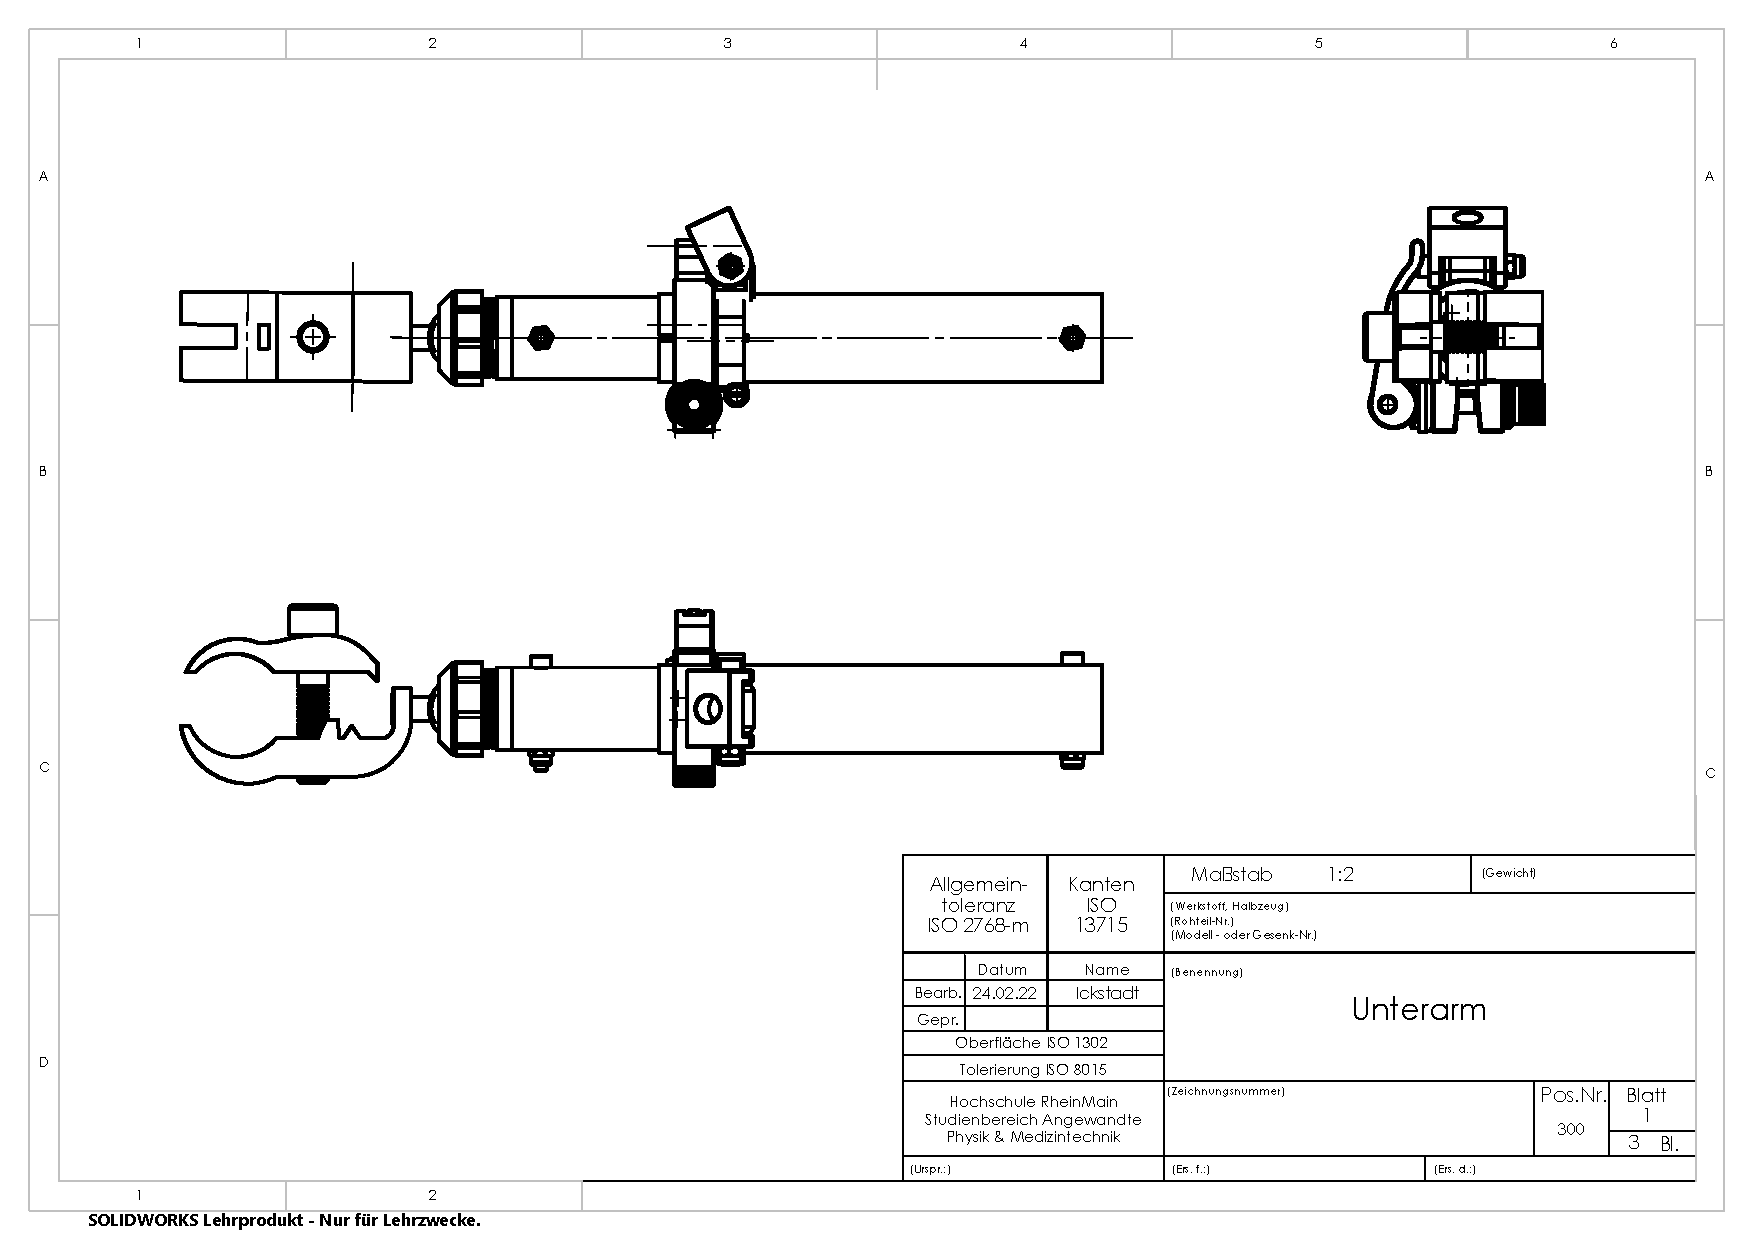
\includepdf[pages=1-2, angle=90, pagecommand={\thispagestyle{plain}}, addtolist={1, figure, Unterarm, drw:Unterarm}]{Abb/CAD/Drawings/Unterarm.pdf}
\includepdf[pages=3, angle=0, pagecommand={\thispagestyle{plain}}]{Abb/CAD/Drawings/Unterarm.pdf}
%
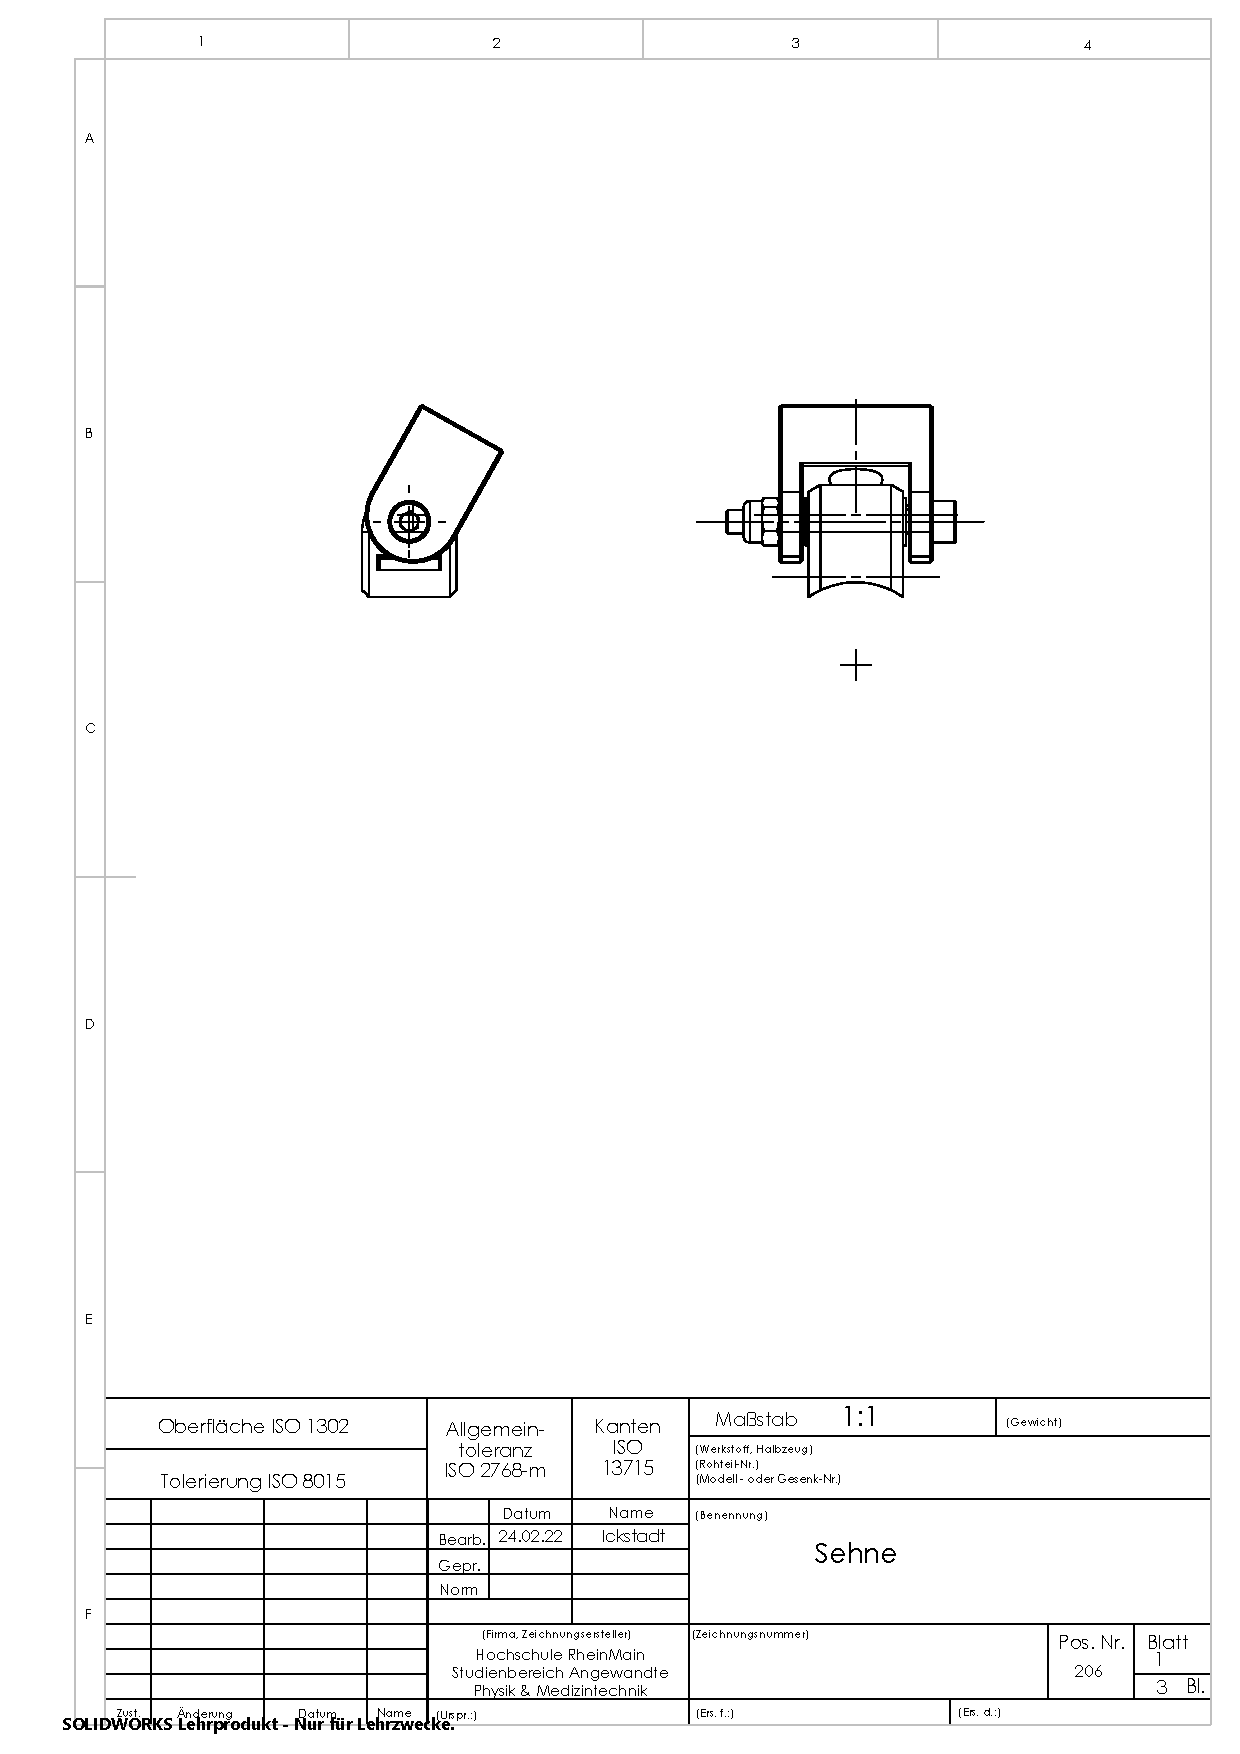
\includepdf[pages=-, angle=0, pagecommand={\thispagestyle{plain}}, addtolist={1, figure, Sehne, drw:Sehne}]{Abb/CAD/Drawings/Sehne.pdf}
%
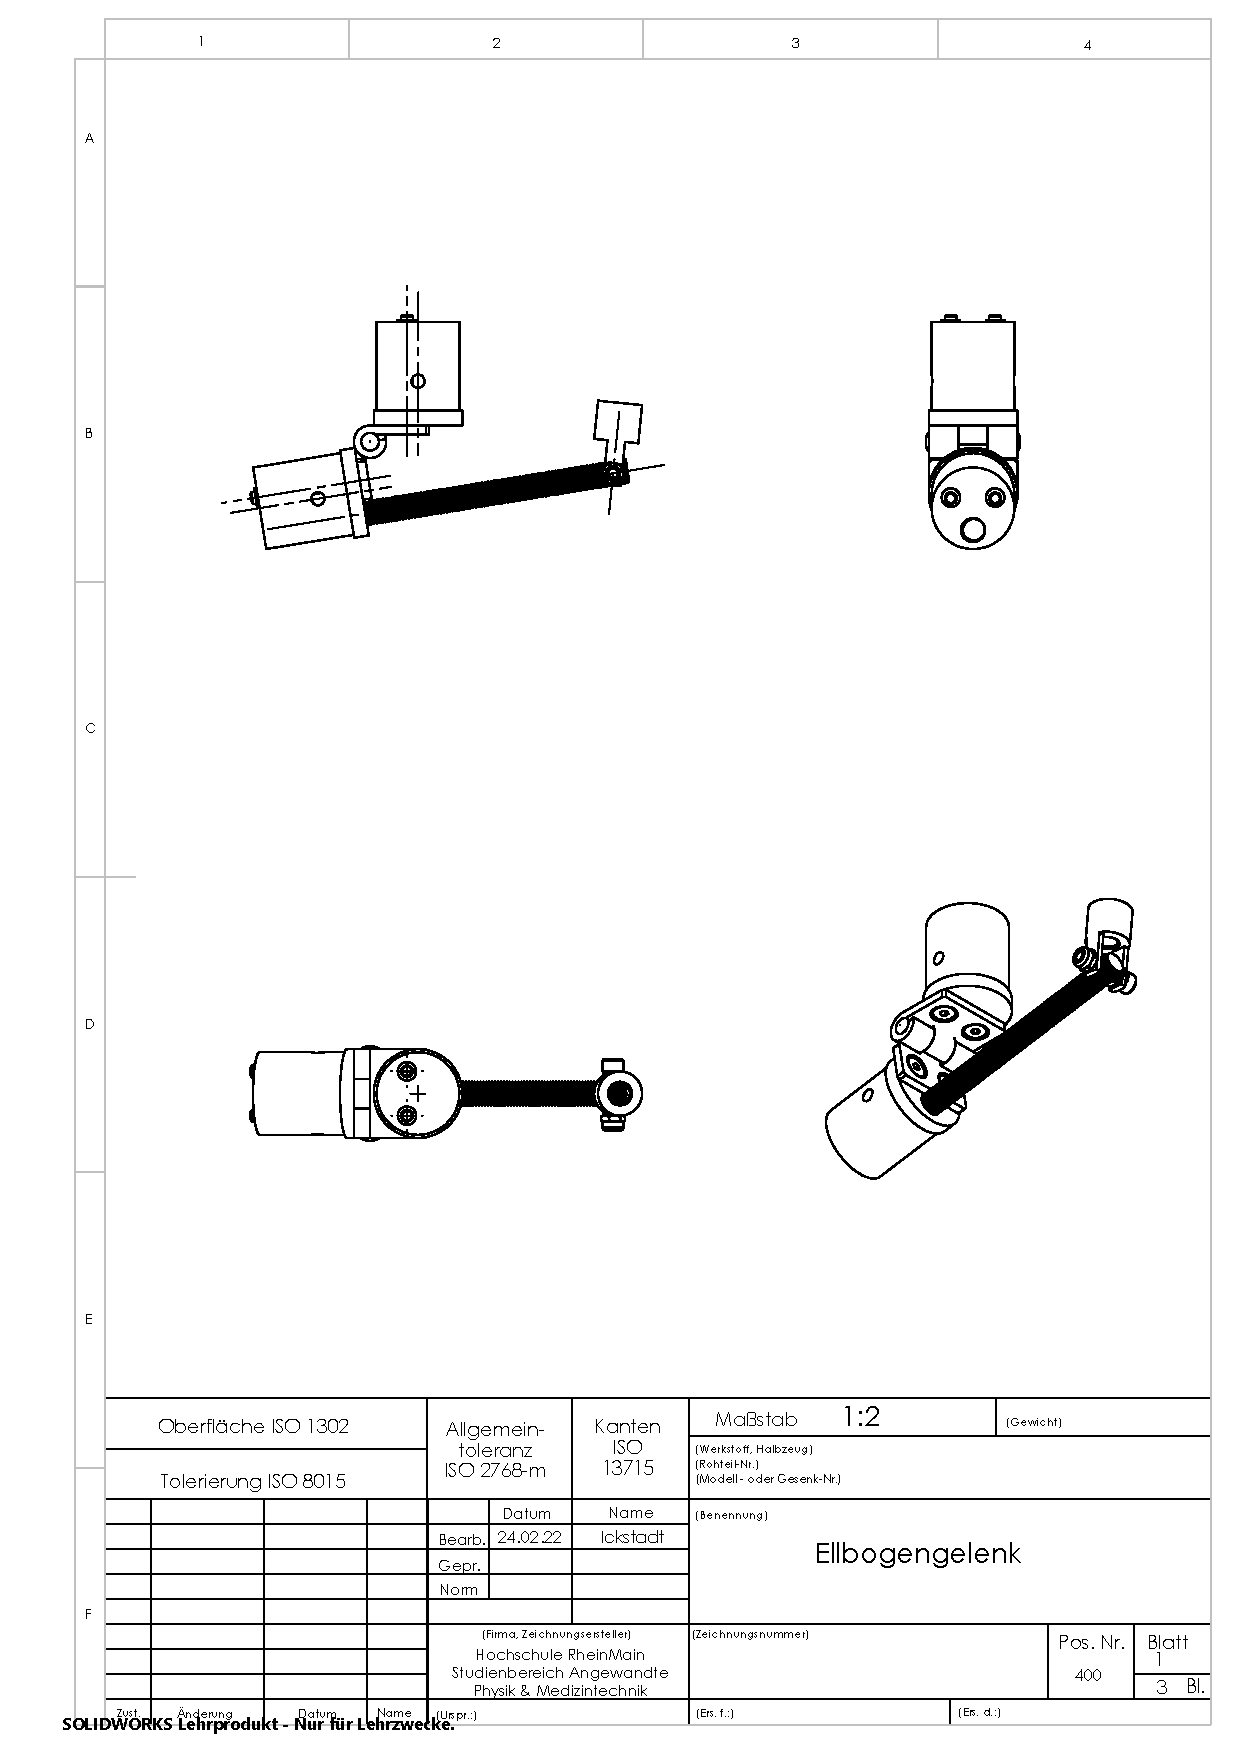
\includepdf[pages=-, angle=0, pagecommand={\thispagestyle{plain}}, addtolist={1, figure, Ellbogengelenk, drw:Ellbogengelenk}]{Abb/CAD/Drawings/Ellbogengelenk.pdf}
%
\includepdf[pages=-, angle=0, pagecommand={\thispagestyle{plain}}, addtolist={1, figure, Exzenter, drw:Exzenter}, addtotoc={1, section, 1, Einzelteilzeichnungen Schultergelenk, {sec:einzelteilzeichnungen schultergelenk}}]{Abb/CAD/Drawings/Schulter/Exzenter.pdf}
%
\includepdf[pages=-, angle=90, pagecommand={\thispagestyle{plain}}, addtolist={1, figure, Motor- und Fixierplatte, drw:Motor und Fixierplatte}]{Abb/CAD/Drawings/Schulter/Motorplatte-Fixierplatte.pdf}
%
\includepdf[pages=-, angle=0, pagecommand={\thispagestyle{plain}}, addtolist={1, figure, Rotor, drw:Rotor}]{Abb/CAD/Drawings/Schulter/Rotor.pdf}
%
\includepdf[pages=-, angle=0, pagecommand={\thispagestyle{plain}}, addtolist={1, figure, Zylinderstift, drw:Zylinderstift}]{Abb/CAD/Drawings/Schulter/Zylinderstift-mit-Innengewinde.pdf}
%
\includepdf[pages=-, angle=0, pagecommand={\thispagestyle{plain}}, addtolist={1, figure, Zahnscheibe, drw:Scheibe}]{Abb/CAD/Drawings/Schulter/Scheibe.pdf}
%
\includepdf[pages=-, angle=90, pagecommand={\thispagestyle{plain}}, addtolist={1, figure, Muskelanschluss, drw:Muskelanschluss}, addtotoc={1, section, 1, Einzelteilzeichnungen Arme, {sec:einzelteilzeichnungen arme}}]{Abb/CAD/Drawings/Anschluss-Muskel-statisch.pdf}
%
\includepdf[pages=-, angle=90, pagecommand={\thispagestyle{plain}}, addtolist={1, figure, Muskelanschluss drehbar, drw:Muskelanschluss-drehbar}]{Abb/CAD/Drawings/Muskelanschluss-drehbar.pdf}
%
\includepdf[pages=-, angle=0, pagecommand={\thispagestyle{plain}}, addtolist={1, figure, Anschluss-Muskel, drw:Anschluss-Muskel}]{Abb/CAD/Drawings/Anschluss-Muskel.pdf}
%
\includepdf[pages=-, angle=90, pagecommand={\thispagestyle{plain}}, addtolist={1, figure, Aussenrohr, drw:Aussenrohr}]{Abb/CAD/Drawings/Aussenrohr.pdf}
%
\includepdf[pages=-, angle=90, pagecommand={\thispagestyle{plain}}, addtolist={1, figure, Oberarminnenrohr, drw:Oberarminnenrohr}]{Abb/CAD/Drawings/Oberarminnenrohr.pdf}
%
\includepdf[pages=-, angle=90, pagecommand={\thispagestyle{plain}}, addtolist={1, figure, Unterarminnenrohr, drw:Unterarminnenrohr}]{Abb/CAD/Drawings/Unterarminnenrohr.pdf}
%
\includepdf[pages=-, angle=0, pagecommand={\thispagestyle{plain}}, addtolist={1, figure, Gelenk-Queue, drw:Gelenk-Queue}]{Abb/CAD/Drawings/Gelenk-Queue.pdf}
%
\includepdf[pages=-, angle=0, pagecommand={\thispagestyle{plain}}, addtolist={1, figure, Queue-Halter, drw:Queue-Halter}]{Abb/CAD/Drawings/Queue-Halter.pdf}
%
\includepdf[pages=-, angle=0, pagecommand={\thispagestyle{plain}}, addtolist={1, figure, Überwurfmutter, drw:Ueberwurfmutter}]{Abb/CAD/Drawings/Ueberwurfmutter.pdf}
%
\includepdf[pages=-, angle=0, pagecommand={\thispagestyle{plain}}, addtolist={1, figure, Gewindestange, drw:Gewindestange}, addtotoc={1, section, 1, Einzelteilzeichnungen Ellbogengelenk, {sec:einzelteilzeichnungen ellbogengelenk}}]{Abb/CAD/Drawings/Gewindestange.pdf}
%
\includepdf[pages=-, angle=0, pagecommand={\thispagestyle{plain}}, addtolist={1, figure, Rohrteil für Ellbogengelenk, drw:Rohrteil-fuer-Ellbogengelenk}]{Abb/CAD/Drawings/Rohrteil-fuer-Ellbogengelenk.pdf}
%
\includepdf[pages=-, angle=90, pagecommand={\thispagestyle{plain}}, addtolist={1, table, Stückliste Pneumatik, tab:StuecklistePneumatik}, addtotoc={1, section, 1, Generelle Stückliste und Pneumatikschaltplan, sec:stueckliste und pneumatikschaltplan}]{Abb/Stuecklisten/StuecklistePneumatik.pdf}
%
\includepdf[pages=-, angle=90, pagecommand={\thispagestyle{plain}}, addtolist={1, figure, Pneumatikschaltplan, drw:PneumatikZeichnung}]{Abb/PneumatikZeichnung.pdf}
%
\includepdf[pages=-, angle=90, pagecommand={\thispagestyle{plain}}, addtolist={1, table, Stückliste Elektrik, tab:StuecklisteElektrik}]{Abb/Stuecklisten/StuecklisteElektrik.pdf}
%
\includepdf[pages=-, angle=90, pagecommand={\thispagestyle{plain}}, addtolist={1, table, Stückliste Mechanik, tab:StuecklisteMech}]{Abb/Stuecklisten/StuecklisteMech.pdf}
\newpage
\setlength{\voffset}{-2.5 cm}
\setlength{\hoffset}{-2 cm}
\chapter{Zeichnungen}\label{sec:zeichnungen}
\newpage
\setlength{\voffset}{0cm}
\setlength{\hoffset}{0cm}
%
\includepdf[pages=1, angle=90, pagecommand={\thispagestyle{plain}}, addtolist={1, figure, Übersicht und Stückliste, drw:Uebersicht und Stueckliste}, addtotoc={1, section, 1, Bauteilzeichnungen, sec:bauteilzeichnungen}]{Abb/CAD/Drawings/Uebersicht-und-Stueckliste.pdf}
\includepdf[pages=2, angle=90, pagecommand={\thispagestyle{plain}}]{Abb/CAD/Drawings/Uebersicht-und-Stueckliste.pdf}
%
\includepdf[pages=1, angle=90, pagecommand={\thispagestyle{plain}}, addtolist={1, figure, Effektor, drw:Effektor}]{Abb/CAD/Drawings/Schulter/Effektor-assembly-drawing.pdf}
\includepdf[pages=2-3, angle=0, pagecommand={\thispagestyle{plain}}]{Abb/CAD/Drawings/Schulter/Effektor-assembly-drawing.pdf}
%
\includepdf[pages=1-2, angle=90, pagecommand={\thispagestyle{plain}}, addtolist={1, figure, Oberarm, drw:Oberarm}]{Abb/CAD/Drawings/Oberarm.pdf}
\includepdf[pages=3, angle=0, pagecommand={\thispagestyle{plain}}]{Abb/CAD/Drawings/Oberarm.pdf}
%
\includepdf[pages=1-2, angle=90, pagecommand={\thispagestyle{plain}}, addtolist={1, figure, Unterarm, drw:Unterarm}]{Abb/CAD/Drawings/Unterarm.pdf}
\includepdf[pages=3, angle=0, pagecommand={\thispagestyle{plain}}]{Abb/CAD/Drawings/Unterarm.pdf}
%
\includepdf[pages=-, angle=0, pagecommand={\thispagestyle{plain}}, addtolist={1, figure, Sehne, drw:Sehne}]{Abb/CAD/Drawings/Sehne.pdf}
%
\includepdf[pages=-, angle=0, pagecommand={\thispagestyle{plain}}, addtolist={1, figure, Ellbogengelenk, drw:Ellbogengelenk}]{Abb/CAD/Drawings/Ellbogengelenk.pdf}
%
\includepdf[pages=-, angle=0, pagecommand={\thispagestyle{plain}}, addtolist={1, figure, Exzenter, drw:Exzenter}, addtotoc={1, section, 1, Einzelteilzeichnungen Schultergelenk, sec:einzelteilzeichnungen schultergelenk}]{Abb/CAD/Drawings/Schulter/Exzenter.pdf}
%
\includepdf[pages=-, angle=90, pagecommand={\thispagestyle{plain}}, addtolist={1, figure, Motor- und Fixierplatte, drw:Motor und Fixierplatte}]{Abb/CAD/Drawings/Schulter/Motorplatte-Fixierplatte.pdf}
%
\includepdf[pages=-, angle=0, pagecommand={\thispagestyle{plain}}, addtolist={1, figure, Rotor, drw:Rotor}]{Abb/CAD/Drawings/Schulter/Rotor.pdf}
%
\includepdf[pages=-, angle=0, pagecommand={\thispagestyle{plain}}, addtolist={1, figure, Zylinderstift, drw:Zylinderstift}]{Abb/CAD/Drawings/Schulter/Zylinderstift-mit-Innengewinde.pdf}
%
\includepdf[pages=-, angle=0, pagecommand={\thispagestyle{plain}}, addtolist={1, figure, Zahnscheibe, drw:Scheibe}]{Abb/CAD/Drawings/Schulter/Scheibe.pdf}
%
\includepdf[pages=-, angle=90, pagecommand={\thispagestyle{plain}}, addtolist={1, figure, Muskelanschluss, drw:Muskelanschluss}, addtotoc={1, section, 1, Einzelteilzeichnungen Arme, sec:einzelteilzeichnungen arme}]{Abb/CAD/Drawings/Anschluss-Muskel-statisch.pdf}
%
\includepdf[pages=-, angle=90, pagecommand={\thispagestyle{plain}}, addtolist={1, figure, Muskelanschluss drehbar, drw:Muskelanschluss-drehbar}]{Abb/CAD/Drawings/Muskelanschluss-drehbar.pdf}
%
\includepdf[pages=-, angle=0, pagecommand={\thispagestyle{plain}}, addtolist={1, figure, Anschluss-Muskel, drw:Anschluss-Muskel}]{Abb/CAD/Drawings/Anschluss-Muskel.pdf}
%
\includepdf[pages=-, angle=90, pagecommand={\thispagestyle{plain}}, addtolist={1, figure, Aussenrohr, drw:Aussenrohr}]{Abb/CAD/Drawings/Aussenrohr.pdf}
%
\includepdf[pages=-, angle=90, pagecommand={\thispagestyle{plain}}, addtolist={1, figure, Oberarminnenrohr, drw:Oberarminnenrohr}]{Abb/CAD/Drawings/Oberarminnenrohr.pdf}
%
\includepdf[pages=-, angle=90, pagecommand={\thispagestyle{plain}}, addtolist={1, figure, Unterarminnenrohr, drw:Unterarminnenrohr}]{Abb/CAD/Drawings/Unterarminnenrohr.pdf}
%
\includepdf[pages=-, angle=0, pagecommand={\thispagestyle{plain}}, addtolist={1, figure, Gelenk-Queue, drw:Gelenk-Queue}]{Abb/CAD/Drawings/Gelenk-Queue.pdf}
%
\includepdf[pages=-, angle=0, pagecommand={\thispagestyle{plain}}, addtolist={1, figure, Queue-Halter, drw:Queue-Halter}]{Abb/CAD/Drawings/Queue-Halter.pdf}
%
\includepdf[pages=-, angle=0, pagecommand={\thispagestyle{plain}}, addtolist={1, figure, Überwurfmutter, drw:Ueberwurfmutter}]{Abb/CAD/Drawings/Ueberwurfmutter.pdf}
%
\includepdf[pages=-, angle=0, pagecommand={\thispagestyle{plain}}, addtolist={1, figure, Gewindestange, drw:Gewindestange}, addtotoc={1, section, 1, Einzelteilzeichnungen Ellbogengelenk, sec:einzelteilzeichnungen ellbogengelenk}]{Abb/CAD/Drawings/Gewindestange.pdf}
%
\includepdf[pages=-, angle=0, pagecommand={\thispagestyle{plain}}, addtolist={1, figure, Rohrteil für Ellbogengelenk, drw:Rohrteil-fuer-Ellbogengelenk}]{Abb/CAD/Drawings/Rohrteil-fuer-Ellbogengelenk.pdf}
%
\includepdf[pages=-, angle=90, pagecommand={\thispagestyle{plain}}, addtolist={1, table, Stückliste Pneumatik, tab:StuecklistePneumatik}, addtotoc={1, section, 1, Generelle Stückliste und Pneumatikschaltplan, sec:stueckliste und pneumatikschaltplan}]{Abb/Stuecklisten/StuecklistePneumatik.pdf}
%
\includepdf[pages=-, angle=90, pagecommand={\thispagestyle{plain}}, addtolist={1, figure, Pneumatikschaltplan, drw:PneumatikZeichnung}]{Abb/PneumatikZeichnung.pdf}
%
\includepdf[pages=-, angle=90, pagecommand={\thispagestyle{plain}}, addtolist={1, table, Stückliste Elektrik, tab:StuecklisteElektrik}]{Abb/Stuecklisten/StuecklisteElektrik.pdf}
%
\includepdf[pages=-, angle=90, pagecommand={\thispagestyle{plain}}, addtolist={1, table, Stückliste Mechanik, tab:StuecklisteMech}]{Abb/Stuecklisten/StuecklisteMech.pdf}
\newpage
\setlength{\voffset}{-2.5 cm}
\setlength{\hoffset}{-2 cm}
\printbibliography%
%=================================================================
\end{document}